%-----------------------------------------------------------------------------------------------------------------------------------------

% PACKAGES
%Document Class starts every LaTeX document.  In this case, we're declaring the document class to be a book.  Changing "oneside" to "twoside" changes where the page numbers and headers and such get placed.
\documentclass[12pt,oneside]{book}

%These are the packages I used.  There's a description of (most of) them below (that Arthur wrote):
\usepackage{fancyhdr, geometry, graphicx, epstopdf, lscape, setspace, amssymb, amsmath, wasysym, moreverb, titlesec, longtable, multirow, alltt, here, indentfirst, ifthen, rotating, bm, afterpage, gensymb, booktabs, array}
\usepackage{hyperref,natbib}
\usepackage[section]{placeins}
\usepackage[flushleft]{threeparttable}
%\usepackage[small,bf]{caption}
\usepackage{subcaption, wrapfig}
\usepackage{tabulary}

%\PassOptionsToPackage{square,numbers}{natbib}
%\RequirePackage{natbib}

% Where to look for figures
\graphicspath{ {Figures/} }

\usepackage[section]{placeins}
\usepackage[small,bf]{caption}
\geometry{letterpaper}



%The "raggedbottom" command allows LaTeX to take some liberty with where the text on a page ends. This saved me some weird formatting problems I was having.
\raggedbottom

%set the pagestyle:
\fancypagestyle{plain}{
\fancyhf{} % clear all header and footer fields, we will re-format them later

%Some formatting stuff:
\renewcommand{\headrulewidth}{0pt}
\renewcommand{\footrulewidth}{0pt}}

% journal defs
\newcommand{\aap}{{\it A\&A}}
\newcommand{\aaps}{{\it A\&AS}}
\newcommand{\aj}{{\it AJ}}
\newcommand{\apj}{{\it ApJ}}
\newcommand{\apjl}{{\it ApJL}}
\newcommand{\apjs}{{\it ApJS}}
\newcommand{\araa}{{\it ARA\&A}}
\newcommand{\iaucirc}{{\it IAU Circular}}
\newcommand{\mnras}{{\it MNRAS}}
\newcommand{\nat}{{\it Nature}}
\newcommand{\pasj}{{\it PASJ}}
\newcommand{\pasp}{{\it PASP}}
\newcommand{\ssr}{{\it SSRv}}
\newcommand{\sciam}{{\it Scientific American}}
\newcommand{\jgr}{{\it JGR}}
\newcommand{\grl}{{\it GRL}}
\newcommand{\icarus}{{\it ICAR}}
\newcommand{\na}{{\it NA}}
\newcommand{\actaa}{{\it ACA}}
\newcommand{\apss}{{\it Ap\&SS}}
\newcommand{\kms}{{km s$^{-1}~$}}


\def\chapterautorefname{Chapter}%
\def\sectionautorefname{Section}%

%name of the space missions


\newcommand{\tess}{\textit{TESS~}}
\newcommand{\kepler}{\textit{Kepler~}}
\newcommand{\ketu}{\textit{K2~}}
\newcommand{\jwst}{\textit{JWST~}}
\newcommand{\spitzer}{\textit{Spitzer~}}
\newcommand{\gaia}{\textit{Gaia~}}



%-----------------------------------------------------------------------------------------------------------------------------------------
% RULES

% This has something to do with headers and margins and stuff:
\DeclareGraphicsRule{.tif}{png}{.png}{`convert #1 `dirname #1`/`basename #1 .tif`.png}
\textwidth 5.750in \textheight=8.50in \headheight 0.0625in \topmargin 0.0in % book strict

%==============================================================================
% Uncomment below for one sided printing (margins the same on even and odd pages)
\oddsidemargin 0.500in \evensidemargin 0.500in

% Uncomment below for two sided printing (margins different on even and odd pages)
%\oddsidemargin 0.563in \evensidemargin 0.2500in

%This sets how we want the formatting of chapter titles to look (bold face and Huge):
\titleformat{\chapter}{\bf\Huge}
{Chapter \thechapter}{-4.4em}{\\}
\titlespacing*{\chapter}{0pt}{-.57in}{*3}

%This formats the section headings:


\titleformat{\section}{\bf\Large}
{\thesection}{1em}{}
\titlespacing*{\section}{0pt}{*2}{*2}

%Let's double-space the document:
\doublespacing

%And our citation style will be aa (astronomy style):
\citestyle{aa}

%-----------------------------------------------------------------------------------------------------------------------------------------
% DOCUMENT/ TITLE PAGE
%Now the document actually begins:
\begin{document}

%This states that this is the stuff that comes before the real text:
\frontmatter

%Here goes the title page:
\pagestyle{empty}
\begin{titlepage}
\begin{center}
\rule{5.75in}{1pt} \\
\vspace*{-0.125in}
{\large Wesleyan University}
\rule[0.2in]{5.75in}{1pt} \\


\vspace*{0.8in}
%{\LARGE \singlespacing \bf Big Disk Energy} \\
{\LARGE \singlespacing \bf A Clever Title} \\
\vspace*{0.05in}
\vspace*{0.10in}
{\large \vspace*{0.20in}  \singlespacing by \vspace*{.2in}
\\Jonas Powell \\ Class of 2019\\}
\vspace*{0.25in}
\vspace*{0.8in}
{\large \singlespacing A thesis submitted to the\\ faculty of Wesleyan University\\ in partial fulfillment of the requirements for the \\ Degree of Master of Arts\\  \vspace*{-0.15in} }
\vspace*{.25in}
\rule{5.75in}{1pt} \\
\vspace*{-0.125in}
{\large \doublespacing Middletown, Connecticut \hfill April, 2018}
\rule[0.2in]{5.75in}{1pt} \\
\end{center}
\end{titlepage}


\pagebreak


\pagestyle{empty}
\mbox{}
\vspace{.75in}
\hrule

\vspace{2in}


%\begin{minipage}[c]{4in}
\begin{centering}
	\hspace{.25in}
	\parbox{5in}{
		\noindent
		\textit{If people sat outside and looked at the stars each night, I'll bet they'd live a lot differently.}
		\vspace{3pt}

		\begin{flushright}
			{\sc {---Calvin & Hobbes}}\\
			% {\textit{The Hitchhiker's Guide to the Galaxy}}
		\end{flushright}
	}
\end{centering}
\vspace{2.25in}
\hrule
\vfill

\textwidth 5.750in \textheight=8.50in \headheight 0.0625in \topmargin 0.0in % book strict

%\chapter{Acknowlegdements}
% \chapter{I'm going on an adventure!}

I have been blessed with an intense and intensely unexpected journey through Wesleyan. When I marked down ``studio art" as my intended major on my ED Common Application to Wesleyan back in the fall of 2013, I had absolutely no idea that, half a decade later, I would be finishing a masters in astronomy with a physics degree under my belt. It goes without saying that making that transition was one that I absolutely could not have survived without the support of an incredible network of friends, family, and mentors.

I think it is appropriate to first acknowledge the role that Dr. Donald Griswold, my high school physics teacher and mentor, has had on my trajectory. It was through his deep dedication to teaching and sharing that I even considered taking a physics class when I got to Wesleyan, but it is also through his mentorship that I learned to contextualize what I learned in the broader scope of life. It also was, is, and always will be his voice that rings in my head when I get too full of myself, reminding me of the absolute power of humility. His guidance in a time of transitions has had an immense effect on me, for which I am deeply grateful.

% It does, of course, take a great deal more than inspiration to actually push yourself to do something that is wildly uncomfortable and unfamiliar; it takes role models and people ``above" you who are genuinely invested in your success.

I've also been lucky to have had a number of peers who have been mentors to me while at Wes. While many of them will go unnamed here, it is worth recognizing Jesse Lieman-Sifry's influence on my Wesleyan career, first through ultimate frisbee, and soon after through coding, astronomy, and the rest of life. I still often wonder how differently my time here would have been had not he been there to bribe me into learning to code, teach me how to throw frisbees far instead of how to throw frisbees well, and be an open and brutally honest listener in moments of distress. It is because of his guidance, drive, and honesty (and a little bit of competitive grit) that I am made it from that first frisbee practice to where I am now.


Sometimes, too, role models are found in people with whom you are clustered, who are taking the same classes at the same time as you, and yet who seem to have some unique way of seeing through problems, some gift for finding solutions, or some deep passion for spending a day listening to the Grateful Dead and modeling stellar interiors. Cail Daley and Ryan Adler-Levine have been that to me: peers to whom I have looked up and tried to keep up with as best I could. Cail's deep wonder at the world and absolute need to make sense of it has been a constant reminder to me that there is always more to be discovered, while Ryan's endless willingness to share his intellect, humor, and joy with those around him serves as valuable course-corrector in times of need.


% I will be honest and admit that, when I really joined the astronomy department in the fall of my junior year, it was not out of any particularly deep, innate love of space and its workings, but rather because the Wesleyan Astronomy Department is an incredibly special place.

The Wesleyan astronomy department as a whole deserves my thanks, having welcomed me with open arms my junior fall. One piece of the department that I am particularly grateful for, tucked away underneath the Observatory's northwest corner, is Roy Kilgard. The endless hours spent talking over the summer, the brief chats while I was playing hooky from Planetary Science Seminar, and, of course, the never ending tolerance for my nonstop stream of emails reporting my technical glitches has added a richness to my Wesleyan experience that is hard to articulate. Roy's candor, willingness to learn, and deep sense of commitment to making sure that our department works in spite of getting almost no ackowledgement for it are all traits I deeply admire.

% Thanks, too, to Francis Starr, for my year of research and several classes with him. Francis is the embodiment of what a liberal arts science professor should be, both as a deeply competent researcher as well as an incredibly articulate, thoughtful, and passionate teacher.

This, of course, leads me to Meredith Hughes, my advisor. In my first year at Wesleyan, I got a little fed up having to listen to Jesse ramble on and on about how wonderful she was, but now that I've had the good fortune to spend five semesters and two-ish summers with her as my guide to the wild world of radio astronomy, I understand what he meant. Meredith embodies what I would hope to see in a liberal arts science professor: an incredibly competent scholar and researcher individually, but one also deeply committed to her students and making this knowledge that we spend all day and night pursuing accessible. I have no idea how I ended up so lucky as to have her as my advisor for these last few years, but however it happened, I'm glad it did.


Finally, I thank my family. Thanks to Michael and Vera for their wisdom and willingness to let me just wander into their house for days at a time. Thanks to Casey for modeling drive and hard work and for always having a wide smile ready. Thanks to Aidan for our talks and helping me see a more grounded perspective. And thanks to Mom and Dad for everything, from driving down to Wes just for a single meal together to pontificating for 20 minutes on the best way to measure an egg. This support has meant the world to me, and without it I (obviously) wouldn't be here, now, writing this darn thing.








\titlespacing*{\chapter}{0pt}{*2}{*3}



\tableofcontents


\titleformat{\chapter}{\bf\Huge}
{Chapter \thechapter}{-4.4em}{\\}
\titlespacing*{\chapter}{0pt}{*2}{*3}

\titleformat{\section}{\bf\Large}
{\thesection}{1em}{}
\titlespacing*{\section}{0pt}{*2}{*2}



%You can also put in the following, if you wish:
\listoffigures
%\listoftables \pagestyle{empty}



\mainmatter



%-----------------------------------------------------------------------------------------------------------------------------------------
% HEADERS
%This took me forever to figure out properly, and you may want to change it.  There's also different thing you can do if you want doublesided printing.  Your final thesis, as published by the University, is one-sided.


\renewcommand{\chaptermark}[1]{ \markboth{\sc\thechapter.\ #1}{}}

\pagestyle{fancy}
\fancyhead{}
\fancyfoot{}

\fancyhead[L]{\leftmark}
\fancyhead[R]{\thepage}

%==============================================================================
%Number your pages!
\pagenumbering{arabic}

%\pagestyle{empty}
\chapter{Introduction}
\label{chap:introduction}

% To fully understand our history, we would hope to understand 1. how we, individually, became conscious; 2. before that, how we developed into human beings; 3. before that, how life began on Earth; 4. before that, how Earth and the Solar system formed; 5. before that, how the Sun formed; and 6. before that, how the Universe formed. The first and final of these questions are generally beyond the scope of traditional Western science, although some neuroscientists and cosmologists (as well as religious scholars, seekers, and philosophers) still try. The second and penultimate questions - how the species (the host of our consciousness) and the Sun (the host of our bodies) came to be - mirror one another both poetically and in that scientists seem to have a fairly solid grasp on each of them, using Darwin's theories and the Hertzprung-Russell Diagram to chart the evolution of our species and our host star. At the center of these six questions, how Life and Earth came into being, we find another symmetry, perhaps most notably thanks to the fact that it is here that science and (Abrahamic) religion disagree most strongly: to the religious mind, the Earth and Life were divinely Created, drawn out from Nothingness into their current, stable forms, while to modern science, life seems to have been the result of some fortuitous chemical mixing and our home, the Earth, the simple by-product of an inefficient stellar formation process somewhere in the suburbia of a minor galaxy in an infinitely vast Universe, both still evolving and changing.
%
% This thesis is an exploration of a miniscule step in the modern Western science's process of finding an acceptable solution to the question of how the Earth and Solar System formed.


Planetary systems, including our own Solar System, are born from circumstellar disks of gas and dust around young stars. Young ($\leq$ 10Myr) circumstellar disks, known as protoplanetary disks, are easily distinguishable from their older siblings by their large abundance of gas, which typically outweighs the disk's dust by a factor of 100. However, as these disks age they are influenced by gravitational, chemical, and viscous forces, and their gas almost entirely dissipates as they become debris disks, much like our familiar local Solar System's Kuiper Belt and asteroid belt. But while we can observe with relative ease the current state of our local planetary system and debris disks, understanding the process that brought us here is much more difficult. To do so, we must understand the nature of our own disk at its birth, and whether or not that process is a common one that we would expect to see replicated elsewhere. Unraveling this mystery requires that we turn to observations of other comparable protoplanetary disks in order to develop a coherent narrative of disk evolution and, consequently, the conditions necessary for the formation of planetary systems like our own.

To understand the birth of our protoplanetary disk, we must understand the birth of our Sun, as the two are intimately related. Stars form when a region of a molecular cloud develops a gravitational instability sufficient to lead to a runaway collapse \citep{Shu1987}, helped along by macroscopic turbulence in the cloud \citep{MckeeOstriker2007}. In this process, the cloud shrinks by a factor of around ten million on its way down to a star, analagous to shrinking a square the approximate size of Connecticut ($\sim$150x150 km) down to just 15mm on each side. Angular momentum, defined as the product of a system's mass, velocity, and radial extent, must be conserved throughout this process,  leading to a tremendous increase in the collapsing cloud's angular velocity. As the local material begins to self-gravitate, its center forms a dense core which will eventually become a young star\footnote{binaries are also a common outcome in this process; according to \citet{DucheneKraus2013}, approximately half of all stars are found in binary systems.}.

However, if that angular momentum is conserved only through an increase in angular velocity, those velocities will become so large that the star itself will be unable to form, as centrifugal forces pulling outward will become more significant than the gravitation pulling the star in on itself. In order to prevent velocities from becoming this high, stellar jets and disks, made from the collapsing material, will develop to decentralize the system's mass and dissipate its angular momentum.

The resulting disks present flared radial structures, typically extending several hundred AU \citep{VicenteAlves2005}. Since these disks form directly out of the collapse process, they, like their stellar host and the initial molecular cloud, are initially composed almost exclusively of molecular hydrogen, although their chemical evolution is significant and heavily studied\footnote{Improving our understanding of this chemical evolution is also one of the motivating drives of this thesis.}. Temperatures in their outer reaches are typically in the range of 10-100 K; gas masses are inferred to range from ones to tens of Jovian masses \citep{AndrewsWilliams2005}, although this value comes with significant assumptions that are discussed in depth in \S\ref{section:continuum_emission}. Masses for the disks in the present study are calculated in Chapter \ref{chap:results}.


% Meredith:
% You should be more specific about what you mean here by “masses” — really what you mean is an inferred gas mass based on the observed dust flux, converted into a dust mass by an assumed opacity, and then into a gas mass by assuming a 100:1 gas:dust mass ratio.
%
% The three HUGE assumptions that go into this are:
% (1) we know the opacity, which really depends on three main unknowns:
%         - the dust composition
%         - the dust shape
%         - the dust size distribution,
% (2) we are seeing all of the solids, which is almost certainly untrue since an unknown amount is locked up into large, invisible bodies like planetesimals and planets,
% (3) we know the gas:dust mass ratio, which we probably don’t (there’s a whole literature on this, especially recently — Kamber Schwarz’s thesis papers, Ted Bergin’s HD observation of TW Hya, and Jonathan Williams’s student whose name I’m forgetting are a good place to start).
%
% Jonas:
% Establishing the masses of the disk's gas and dust is a multi-step process




\begin{figure}[htp]
  \hspace*{\fill}%
  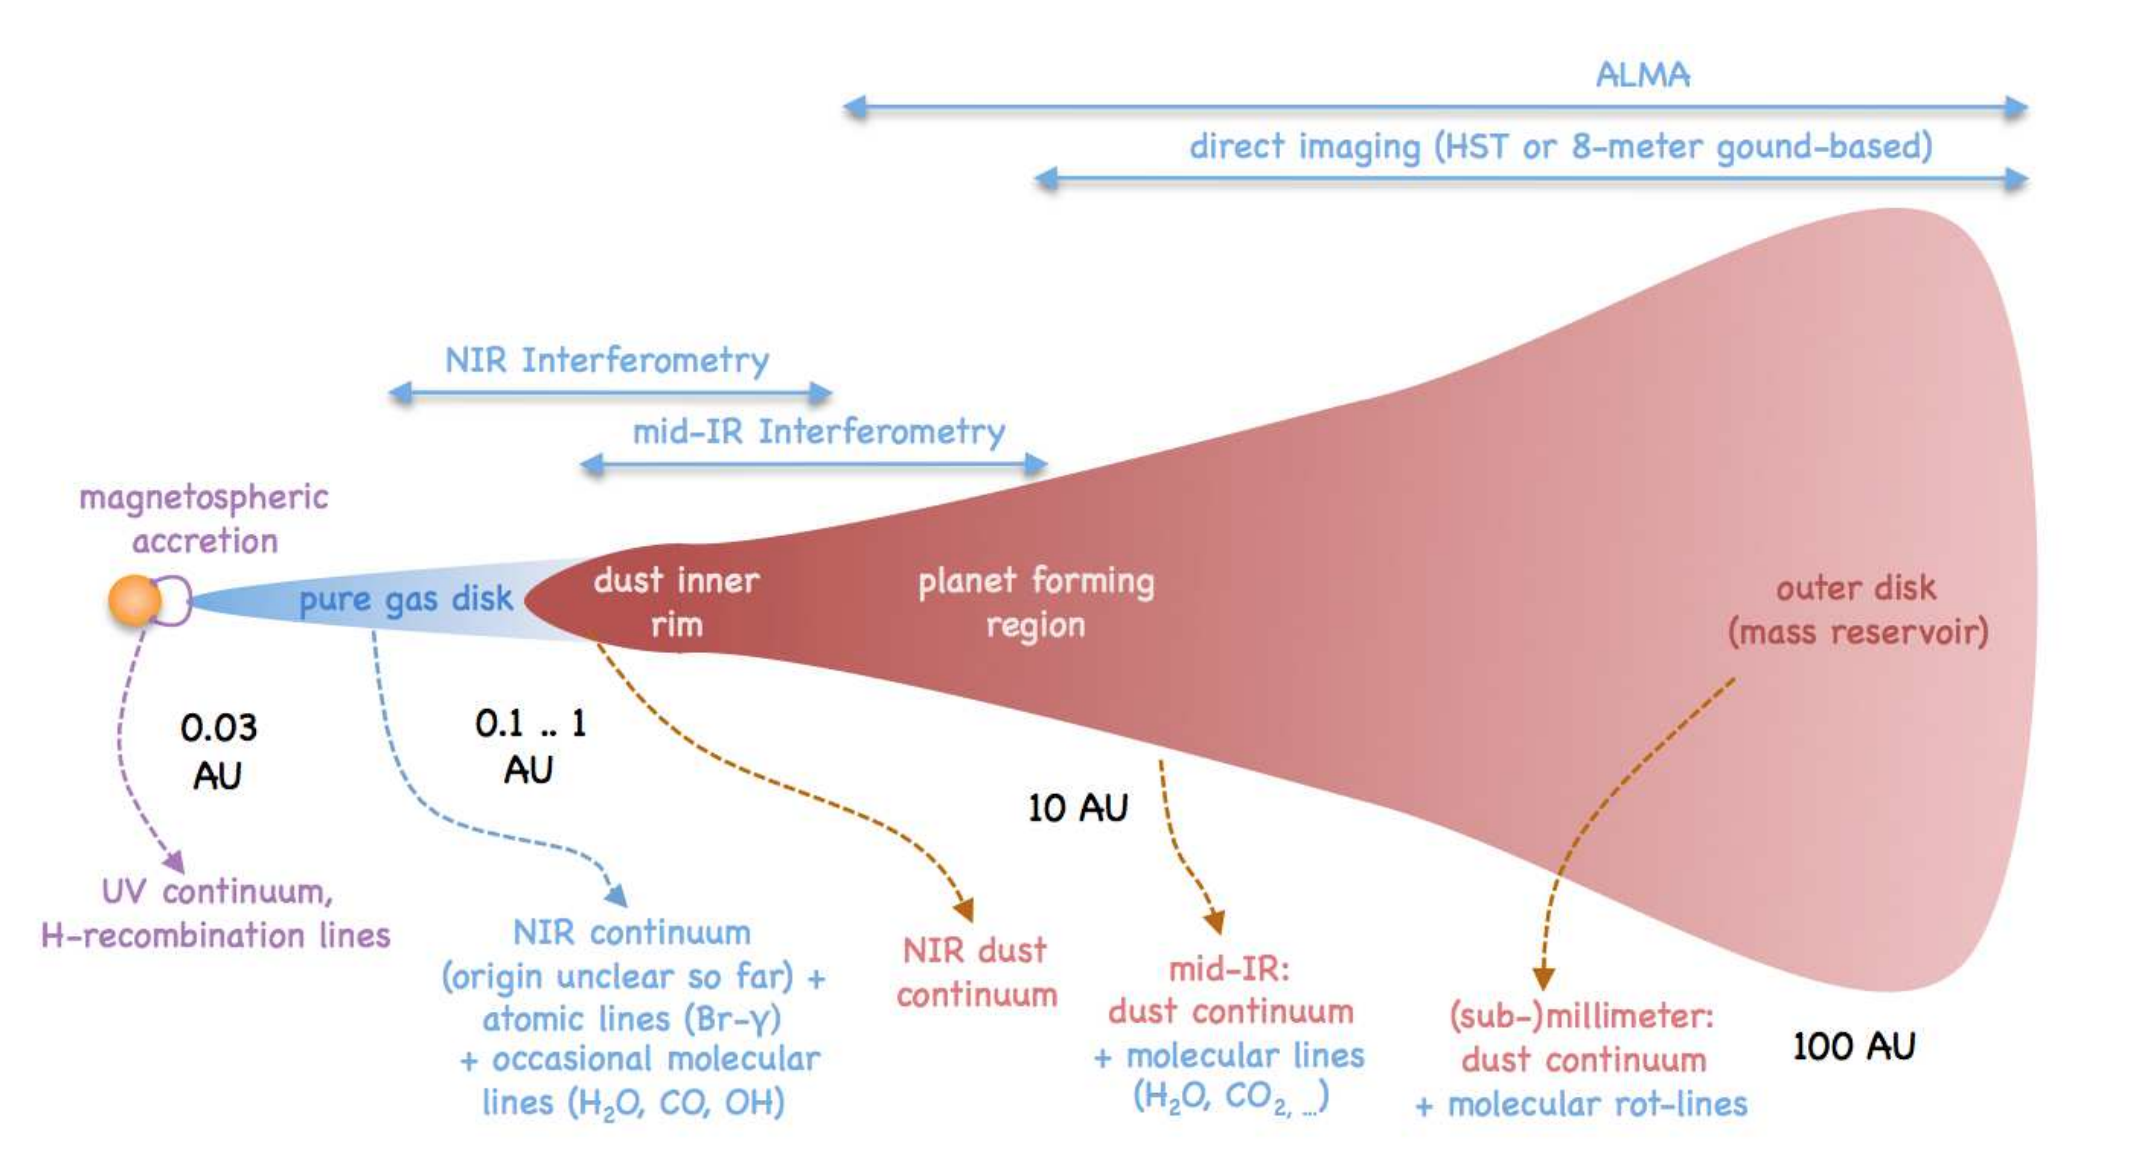
\includegraphics[width=\linewidth]{proplyd_structure.png}\hfill%
  \hspace*{\fill}%
  \label{fig:proplyd_str}
  \captionof{figure}{An edge-on slice of a protoplanetary disk is presented \citep{DullemondMonnier2010}. As is visible in this graphic, significant radial segmentation of the disk exists, particularly between the inner gas disk and outer disk of gas, dust, and planetesimals. Also of note is the large vertical flaring that occurs at large radii. Since the observations that this thesis are based on were made with ALMA (discussed in \S\ref{section:interferometry}), we are sensitive primarily to the outer reaches of the disk.}
\end{figure}



By around 10-20 Myr, the primordial gas and dust in these disks becomes depleted through several processes, including accretion onto the host star, blowing out from radiation pressure, and becoming locked up in icy bodies, transitioning the disk from a protoplanetary disk to a debris disk. These new debris disks are made up of what is thought to be second generation dust, created by the grinding down of boulders and planetesimals, since any primordial dust from the initial collapse should have been blown out by this time. The gas masses in debris disks tend to be orders of magnitude lower than in protoplanetary disks. For a more complete review of disk evolution, see \citet{Hughes2018}.




\section{Submillimeter Observations}

Although protoplanetary disks' masses are dominated by gas, they still have sufficient dust to be optically thick in the optical. Consequently, mass measurements are not possible at optical wavelengths. However, since the optical depth of the dust at millimeter wavelengths is low, and since the emission being observed at these wavelengths is thermal rather than due to scattering (as it is in the optical), observations at millimeter wavelengths are preferred for measuring a disk's dust mass. In the radio, we may trace two types of emission:

\begin{itemize}

  % How do you know that the dust doesn’t absorb at mm wavelengths??? If there’s mm-size dust, it should absorb mm wavelengths!  The small dust grains won’t, but remember that there’s a whole size distribution, and in fact, the balance between the steep size distribution (weighted towards small grains) and the dropoff of emission efficiency (weighted towards large grains) means that the grains we are seeing at mm wavelengths are most likely in fact the mm-size grains that *do* both absorb and emit efficiently at mm wavelengths.

  \item \textsc{Continuum emission}: Although the size distribution of grains in a dust disk is wide and heavily weighted towards smaller grains, larger, millimeter-sized grains are still present in disks. These larger grains are far more efficient emitters in the radio, since the wavelength of a grain's peak thermal emission efficiency is approximately equal to its size. Thus, we may observe this continuum emission (so named thanks to the wide range of frequencies that thermal emission covers) from these millimeter-sized grains.

  % I think it might be good to be specific here that continuum emission is (1) from dust, and (2) thermal in nature (which is why it spans a wide range of frequencies)

  % I don't like this, but maybe it's fine
  \item \textsc{Line emission}: Because radial disk temperatures quickly fall below the temperatures required to cause photodissociation, molecules may live a stable existence in these disks. Conveniently, the rotational transitions of small molecules tend to emit at radio frequencies. Observations of the emission from these rotational transitions, known as line emission, can provide us with a wealth of important information, including kinematics, temperature information, disk chemistry and total disk mass.
\end{itemize}


Notably absent in both forms is emission from the central star, thanks to the fact that stars are extremely weak emitters in the radio regime, since stars are hot and, consequently, have peak emission in the optical\footnote{Why, then, is the dust still bright relative to the star? While it's true that the flux \textit{per area} of the dust is significantly smaller than of the star, the dust has a far greater surface area, allowing it to compensate and still be a bright emitter.}. This makes them very faint relative to the disk's emission at longer (hundreds to thousands of microns) wavelengths. Fig \ref{fig:SED} \citep{Hughes2010} presents a spectral energy distribution, or SED, showing emission intensity as a function of wavelength from an imaginary disk system, demonstrating how small the star's flux density is at long wavelengths relative to the disk's contributions.


\begin{figure}
\centering
  \includegraphics[width=\linewidth]{Meredith_SED.png}
  % 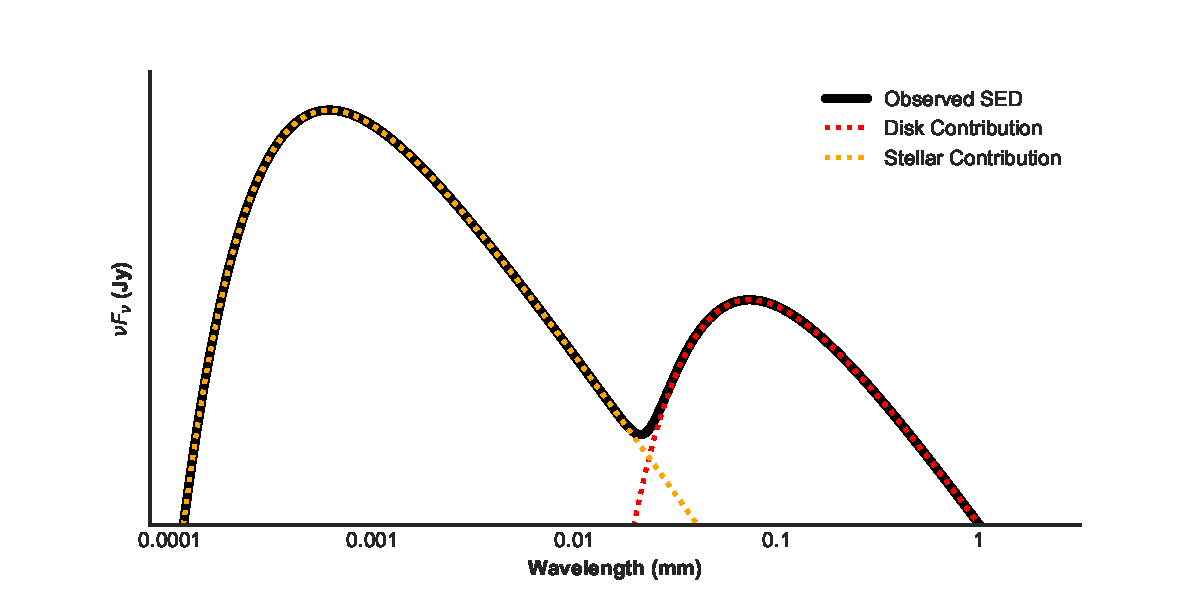
\includegraphics[width=\linewidth]{example_SED.pdf}
  \captionof{figure}{Two example SEDs, accompanied by cartoon models to illustrate the various contributions of different elements of a disk and their influences on the SED \citep{Hughes2010}. The dashed line corresponds to emission from the stellar photosphere, while the colored lines are blackbody curves corresponding to emission from regions of the disk with different temperatures. Since radio observations take place at longer (hundreds to thousands of microns) wavelengths, one may easily see that the stellar contribution in that regime is minimal.}
  \label{fig:SED}
\end{figure}

% Meredith's caption: Cartoon illustrating SED modeling and the association between midIR deficits and inner holes in transition disks. The black solid line shows a model of a T Tauri star surrounded by a disk that (left) extends in to the dust destruction radius or (right) is truncated at 1 AU from the star. The dashed line marks the SED contribution from the stellar photosphere. The colored lines are blackbody curves showing the contribution of dust at different temperatures to the excess over the photosphere: curves with peaks at shorter wavelengths originate from hotter dust. The mid-IR deficit in the figure on the right corresponds to missing emission from the hottest dust. The illustration below each plot shows how the temperature of the dust is related to distance from the star, and highlights the idea that missing short-wavelength emission from the SED corresponds to missing dust close to the star

However, to understand these types of observation, one must first understand the nature of the ``telescope" making the observations. What follows is a brief introduction to radio interferometry, followed by more complete explanations of continuum and line emission.



\subsection{Interferometry}
\label{section:interferometry}
Interferometry is a clever way to make extremely high-resolution observations at long wavelengths without needing to use incredibly large collecting areas. Were one to naively attempt to create a ``traditional" (single-aperture) telescope to capture radio emission, they would quickly recall that, for a telescope with a single circular aperture of diameter $D$, maximum angular resolution is given by
% Ignoring a Meredith comment here about this being a general equation if we replace D with a baseline.
\begin{align}
  \theta &= 1.22 \, \frac{\lambda}{D},
\end{align}

\noindent where $\theta$ is the angular resolution achieved, and $\lambda$ is the wavelength of the emission being observed. Unfortunately, light in the radio regime has wavelengths on the order of millimeters to centimeters, orders of magnitude longer than optical light, which is in the hundreds of nanometers. Consequently, to achieve a resolution comparable to that of an optical telescope, one would have to increase their aperture's diameter accordingly to match the increase in $\lambda$. Some have tried this approach: the Arecibo Observatory in Puerto Rico and the Five hundred meter Aperture Spherical Telescope in China (with diameters of 300m and 500m, respectively) are two immediate examples, but both still have resolutions ($\sim25''$ for Arecibo and $\sim15''$ for FAST, observing 3cm emission) that are too coarse to resolve the length-scales that we would like when observing disks. Building and maintaining apertures this big is also an extreme challenge, usually requiring mountains to be hollowed out, making this an unappealing solution.

%REWORK: Make sure to note that ALMA has lots of big dishes so sensitivity is less of an issue.

The alternative is to leverage the power of interferometry for a solution to the problem. In an interferometric system, one may construct an image using the interference patterns between light received by two or more separate apertures. In this case, the maximum angular resolution becomes inversely proportional to the maximum distance, or \textit{baseline}, between any two  apertures, which can be made almost arbitrarily large. Interferometry does come with tradeoffs, however, the most notable of which is in sensitivity, since sensitivity is proportional to collecting area and each dish in an interferometer is typically fairly small. Additionally, inteferometers also have inherent spatial filtering, meaning that they are not sensitive to flux from sources covering large angular scales. This is because the largest angular scale of a flux source that a telescope is sensitive to is inversely proportional to its smallest baseline. Since the collecting area of a single-dish telescope is a continous surface, its smallest ``baseline" is essentially infinitely small (making it sensitive to arbitrarily-large flux sources). Conversely, for an interferometer, that smallest baseline is typically ones to tens of meters. Therefore, interferometers are intrinsically unable to capture flux from sources with angular scales larger than $\lambda/D_\text{min}$.\footnote{This can actually be an advantage, however, as it offers the opportunity to choose the length-scale being observed, i.e. remove cloud contamination (large scale structure) from an image of a disk (a small structure).}


% Well, it’s only unappealing if you don’t also need the collecting area.  There are certainly advantages to single apertures, chief among them sensitivity, as well as the ability to measure total fluxes (which is why we often want to try to get single-dish flux measurements of ALMA sources, though that doesn’t work in the case of Orion because there’s too much cloud contamination).  IGNORING THIS

% In our case, the resolution is important because disks have angular scales that are too small to resolve with single-dish telescopes, and interferometry also happens to be convenient for highly contaminated molecular cloud regions like Orion — spatial filtering is often listed as one of the drawbacks of interferometers (because we miss flux on large angular scales), but in our case it’s a benefit because it lets us be sensitive to the relatively small-scale structure of the disk while ignoring the large-scale structure of the cloud that would overwhelm a single-dish telescope.

% The tradeoff is lower sensitivity, but ALMA mitigates that somewhat with its large number of dishes (the LNSD design is becoming the gold standard for interferometers, though ALMA’s dishes can’t really be said to be small… though again, that’s not an issue for us, since we don’t need a large field of view to look at tiny disks.  It’s certainly a drawback of interferometry for galaxy observers, though!)



While this interference process can be done at optical wavelengths with CCDs, it is far more difficult to execute, as light must be forced to physically interact before reaching the sensor via a complex and extremely precise optical system. At longer wavelengths, however, heterodyne receivers may be used, making the task of interfering the signals a digital process, rather than a physical one. A heterodyne receiever records both the amplitude (analogous to the intensity that a CCD might measure) and the phase of the signal it receives. Because the receiver captures phase information as well as amplitude, the signals from two dishes may be digitally interfered after being received. Physical features must be calibrated out, including phase delay caused by differences in line-of-sight path length from the source between the receivers, atmospheric effects, and instrumental phase delays. The result, for a single baseline, is a complex voltage pattern describing the amplitude and phase of the interference pattern between the signal each dish received. We call this voltage pattern a \textit{visibility}.


% “is called a visibility and lives in the visibility domain” — just think of how incomprehensible this sentence would have been to you three years ago. :-)

% Maybe start this paragraph with a general statement that what an interferometer records is actually the Fourier transform of an image, and that the visibility domain is the Fourier transform of the image domain.  

The complete output from an interferometer is a collection of these visibilities. Taken together, they approximate the Fourier transform of the sky image. We say that this output lives in the ``visibility domain", which itself is a Fourier transform of the image domain. A single visibility relates to the full set of visibilities analogously to the relationship between a pixel and an image.


While the image domain has spatial dimensions (i.e. the $xy$ plane), the visibility domain instead uses the $uv$ plane. The $uv$ plane is a wavelength-scaled $x-y$ coordinate system parallel to the sky in the direction of the target source. Here ``wavelength-scaled" can be taken to mean that $u = X/\lambda, v = Y/\lambda$, where $\lambda$ is the wavelength of observation and $X$ and $Y$ are the lengths of the $x$ and $y$ (i.e. north/south, east/west) components of the projected baseline. Thus, each baseline samples a specific spatial frequency, given by $\theta = 1/\sqrt{u^2 + v^2}$. An interferometer may thus be represented on the $uv$ plane as a scatter of points, with each point corresponding to the wavelength-scaled, target-projected, component distance between two receivers. The ideal aperture would completely fill the $uv$ plane, so that every spatial frequency was sampled. However, since the number of baselines we may access is very limited (approximately the square of the number of antennae in an array), this is clearly an impossibility for an interferometer.\footnote{Of course, a single-aperture telescope does not have this problem since its $uv$ plane is one continuous collecting area and thus can be seen as having infinite baselines and complete $uv$ coverage.}


However, the fact that the $projected$ baseline is really what determines visibility's location in the $uv$ plane, rather than the baseline's ``true", un-projected length, allows us to cleverly gain far more points in the $uv$ plane than one might immediately expect. Since the Earth rotates throughout the night, the projection of a given baseline relative to the target source will change throughout the night as well. Consequently, by making observations over the course of a night, many more points in the $uv$ plane may be sampled, yielding a better-filled plane. This process is known as ``Earth rotation aperture synthesis."

We now consider how one might recover an image from a set of observed visibilities. In general, moving between frequency space and distance space is given by a simple Fourier transform. When applying this translation to telescopes, we consider the shape of the image produced by observation of a single point source directly on axis with the aperture. For a conventional telescope with a circular aperture, coverage in the $uv$ plane is in the shape of a filled circle of constant amplitude. Translation to the image domain, via a Fourier transform of that shape, results in the familiar 2-D Airy Disk, the characteristic point-spread function (PSF) of a single aperture convolved with a point source. With an interferometer, this process would be equally straightforward if the $uv$ plane were fully sampled, but because it is not, the resulting image is instead a Fourier transform of all the points in the $uv$ plane sampled by the baselines, and can take on a very complex shape\footnote{Additionally, thanks to the incomplete sampling of the $uv$ plane, an infinite number of images could all be consistent with some given finite set of visibilities, although many of them would not be physically possible. The one we choose to look at is determined by our deconvolution process, but is not actually the true image.}. However, while this shape is complex, it is still - as is the case in the optical - just a convolution of the point source with some PSF, only in this case the PSF is more complicated than an Airy function. As we increase the number of $uv$ points sampled, the resulting image will increasingly approximate a bumpy and/or elongated Airy disk. In radio astronomy, we call this PSF the ``dirty beam".

% For above: “can take on a very complex shape” — I wonder if it would be helpful here to introduce the concept of the PSF (or dirty beam) and the fact that the raw image is in fact the convolution of the true image with the PSF (this is true for all telescopes, not just interferometers, so it can be a helpful concept for optical astronomers trying to figure out interferometry).  

When observing a source, we would like to find the true sky brightness pattern (i.e. the sky image). As described above, the Fourier transform of a set of visibilities is a convolution of the dirty beam with the true sky brightness pattern. Therefore, we would like to remove the dirty beam's contributions to the image. The process of removing the influence of the dirty beam, and the artifacts it can introduce, is called deconvolution. In practice, this deconvolution process takes the form of some iterative algorithm that selectively removes the effects of the dirty beam. The curious reader is referred to the CLEAN algorithm \citep{Hogbom1974}, the first and most popular deconvolution algorithm (and the one used in this work), as well as the maximum-entropy method \citep{Wernecke1977,SkillingBryan1984}. It is worth noting at this point, however, that due to the artifacting and non-unique result that the imaging process introduces, all of our analysis is performed directly on the visibilities themselves, rather than the image. This means that the specific parametrization of CLEAN or any other step in the imaging process does not need to be perfect, since it is purely diagnostic or expository.


In summary, interferometry works by recording amplitude and phase information about some emission with many radio antennae and digitally interfering each antenna's signal with the signal received by every other telescope. Each of the resulting interference patterns is called a visibility, and represents a point in $uv$ space. Translation from the visibility domain to the image domain involves taking the Fourier transform of the visibilities and deconvolving the dirty beam's influence.

Currently, the world's most advanced interferometer, and the source of this thesis's data, is the Atacama Large Millimeter/Submillimeter Array (ALMA), shown in Fig \ref{fig:ALMA}. Built in the high Chilean desert at around 5,000 meters (16,000 feet), the \$1.4-billion array first opened its eyes for scientific observation in mid-2011, with funding from a global partnership between Chile, the United States, and several other countries. With its 66 total antennae (50 12-m dishes and 16 7-m dishes) and baselines extending out to 15-km, it offers an order of magnitude increase in sensitivity and resolution over previous arrays that observe at similar frequencies, which include the Submillimeter Array (8 6-meter dishes), NOEMA (10 15-meter dishes) and the CARMA (23 dishes of 3.5-m, 6.1-m, and 10.4-m diameters).

\begin{figure}[htp]
  \hspace*{\fill}%
  \subcaptionbox{\label{fig:ALMA}}{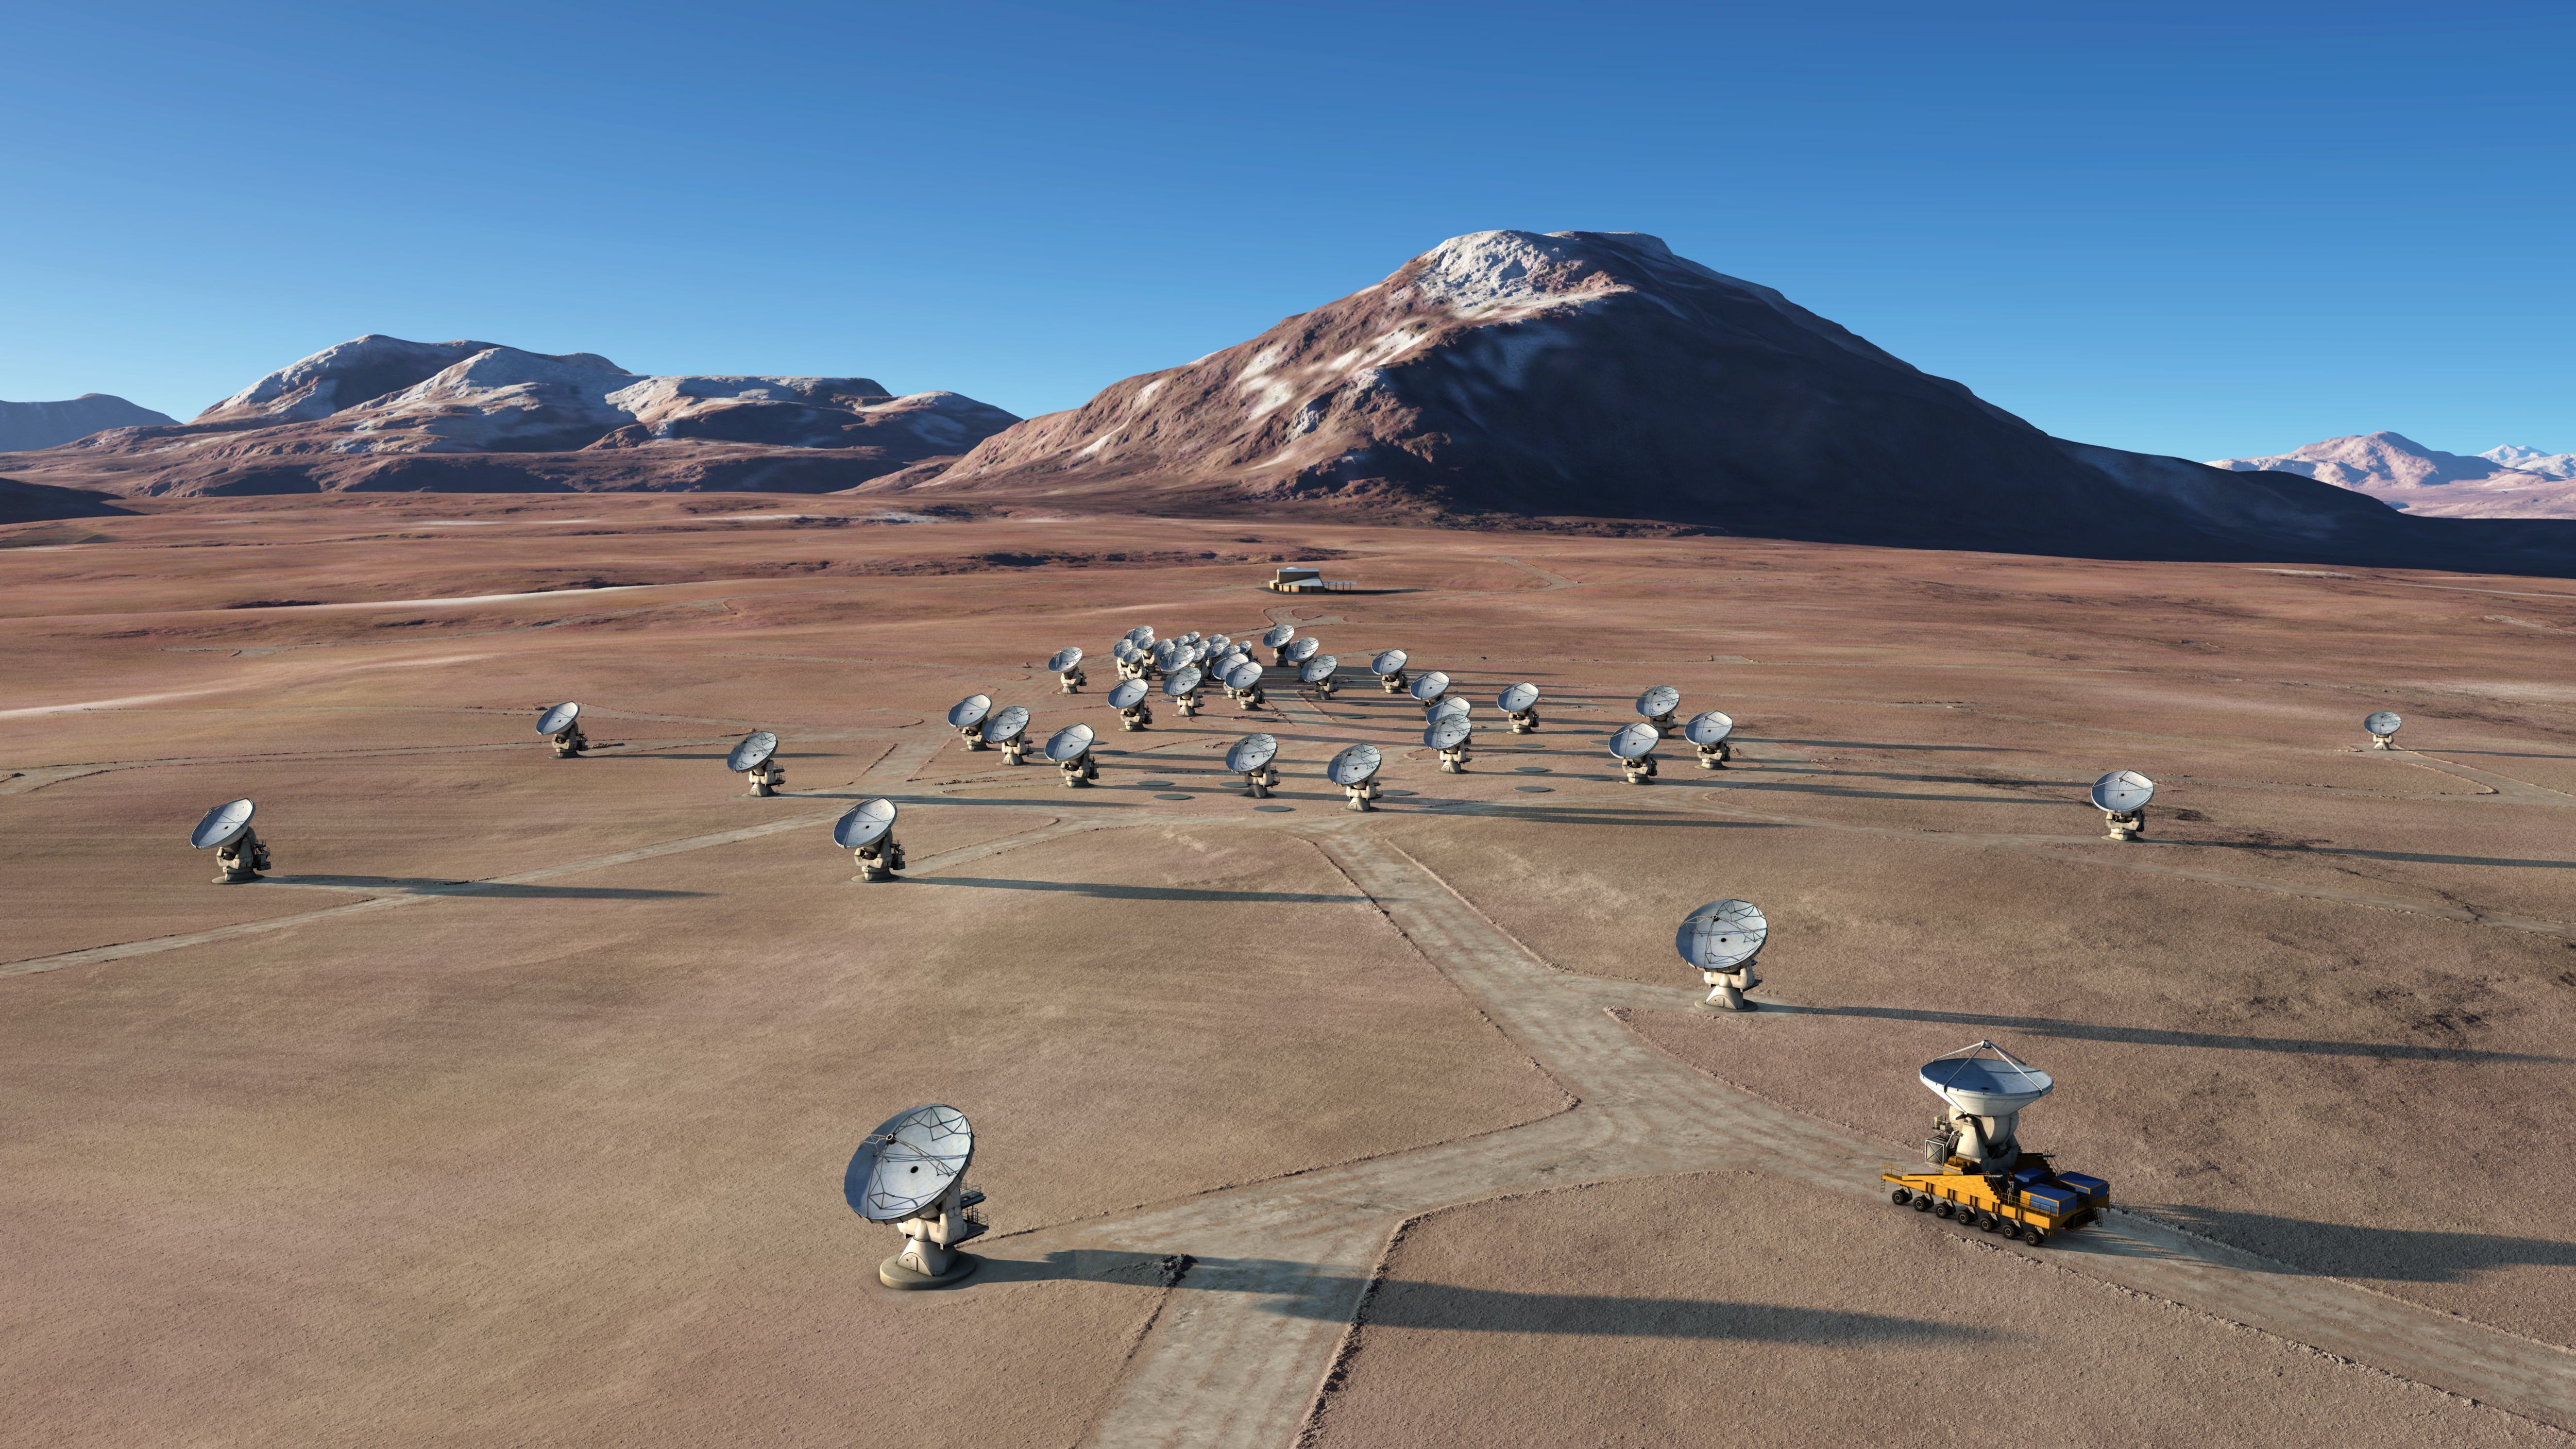
\includegraphics[width=0.5\linewidth]{ALMA_universetoday.jpg}}\hfill%
  \subcaptionbox{\label{fig:Andrews_proplyds}}{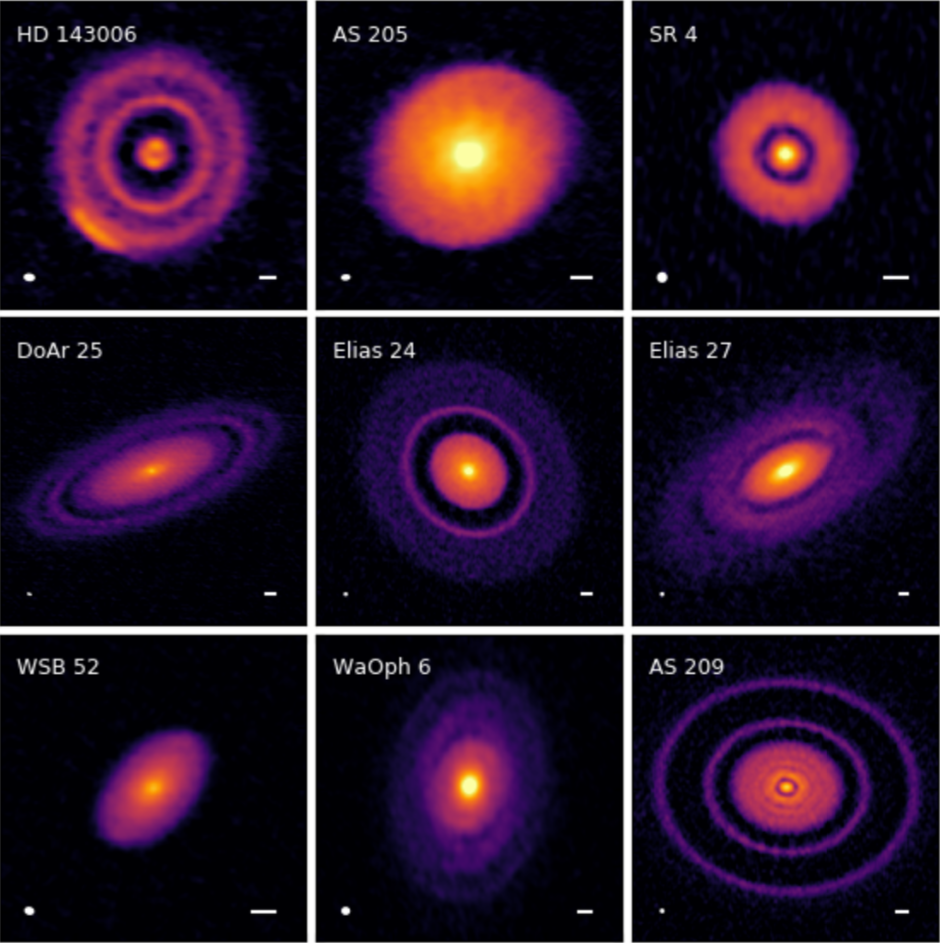
\includegraphics[width=0.3\linewidth]{Andrews2018_proplyds.png}}%
  \hspace*{\fill}%
  \captionof{figure}{\textit{Left:} A rendering of ALMA\footnote{Courtesy of \url{www.almaobservatory.org/en/about-alma-at-first-glance/origins/}} shows the interferometer's antennae in the high desert, as well as a purpose-built truck moving one of the antennae (lower right). \textit{Right:} A recent survey from ALMA by \citet{Andrews2018} reveals stunning detail in several protoplanetary disks.}
\end{figure}


The effects of this increase are impressive; gaps and rings in faraway disks are now resolvable in striking clarity (Fig. \ref{fig:Andrews_proplyds}), providing a treasure-trove of opportunity to hone our understanding of disk evolution and planetary-system formation. ALMA has also been a blessing to other subfields of astronomy as well, enabling high-resolution observations of everything from complex organic molecules in disks \citep{Walsh2016,Podio2019} to gravitational lensing from dark matter halos \citep{Herrera-Martin2019} to molecular tori around black holes \citep{Combes2018}. Additionally, as a component of the Event Horizon Telescope, ALMA played a key role in imaging a black hole's event horizon for the first time \citep{EHTCollab2019}. These awe-inspiring projects are a small portion of ALMAs contributions to the world of radio astronomy, and more are being made with each passing day.


With an improved understanding of the mechanics of radio interferometry, we may now revisit continuum and line emission.

% \begin{figure}
% \centering
% \begin{minipage}{.48\textwidth}
%   \centering
%   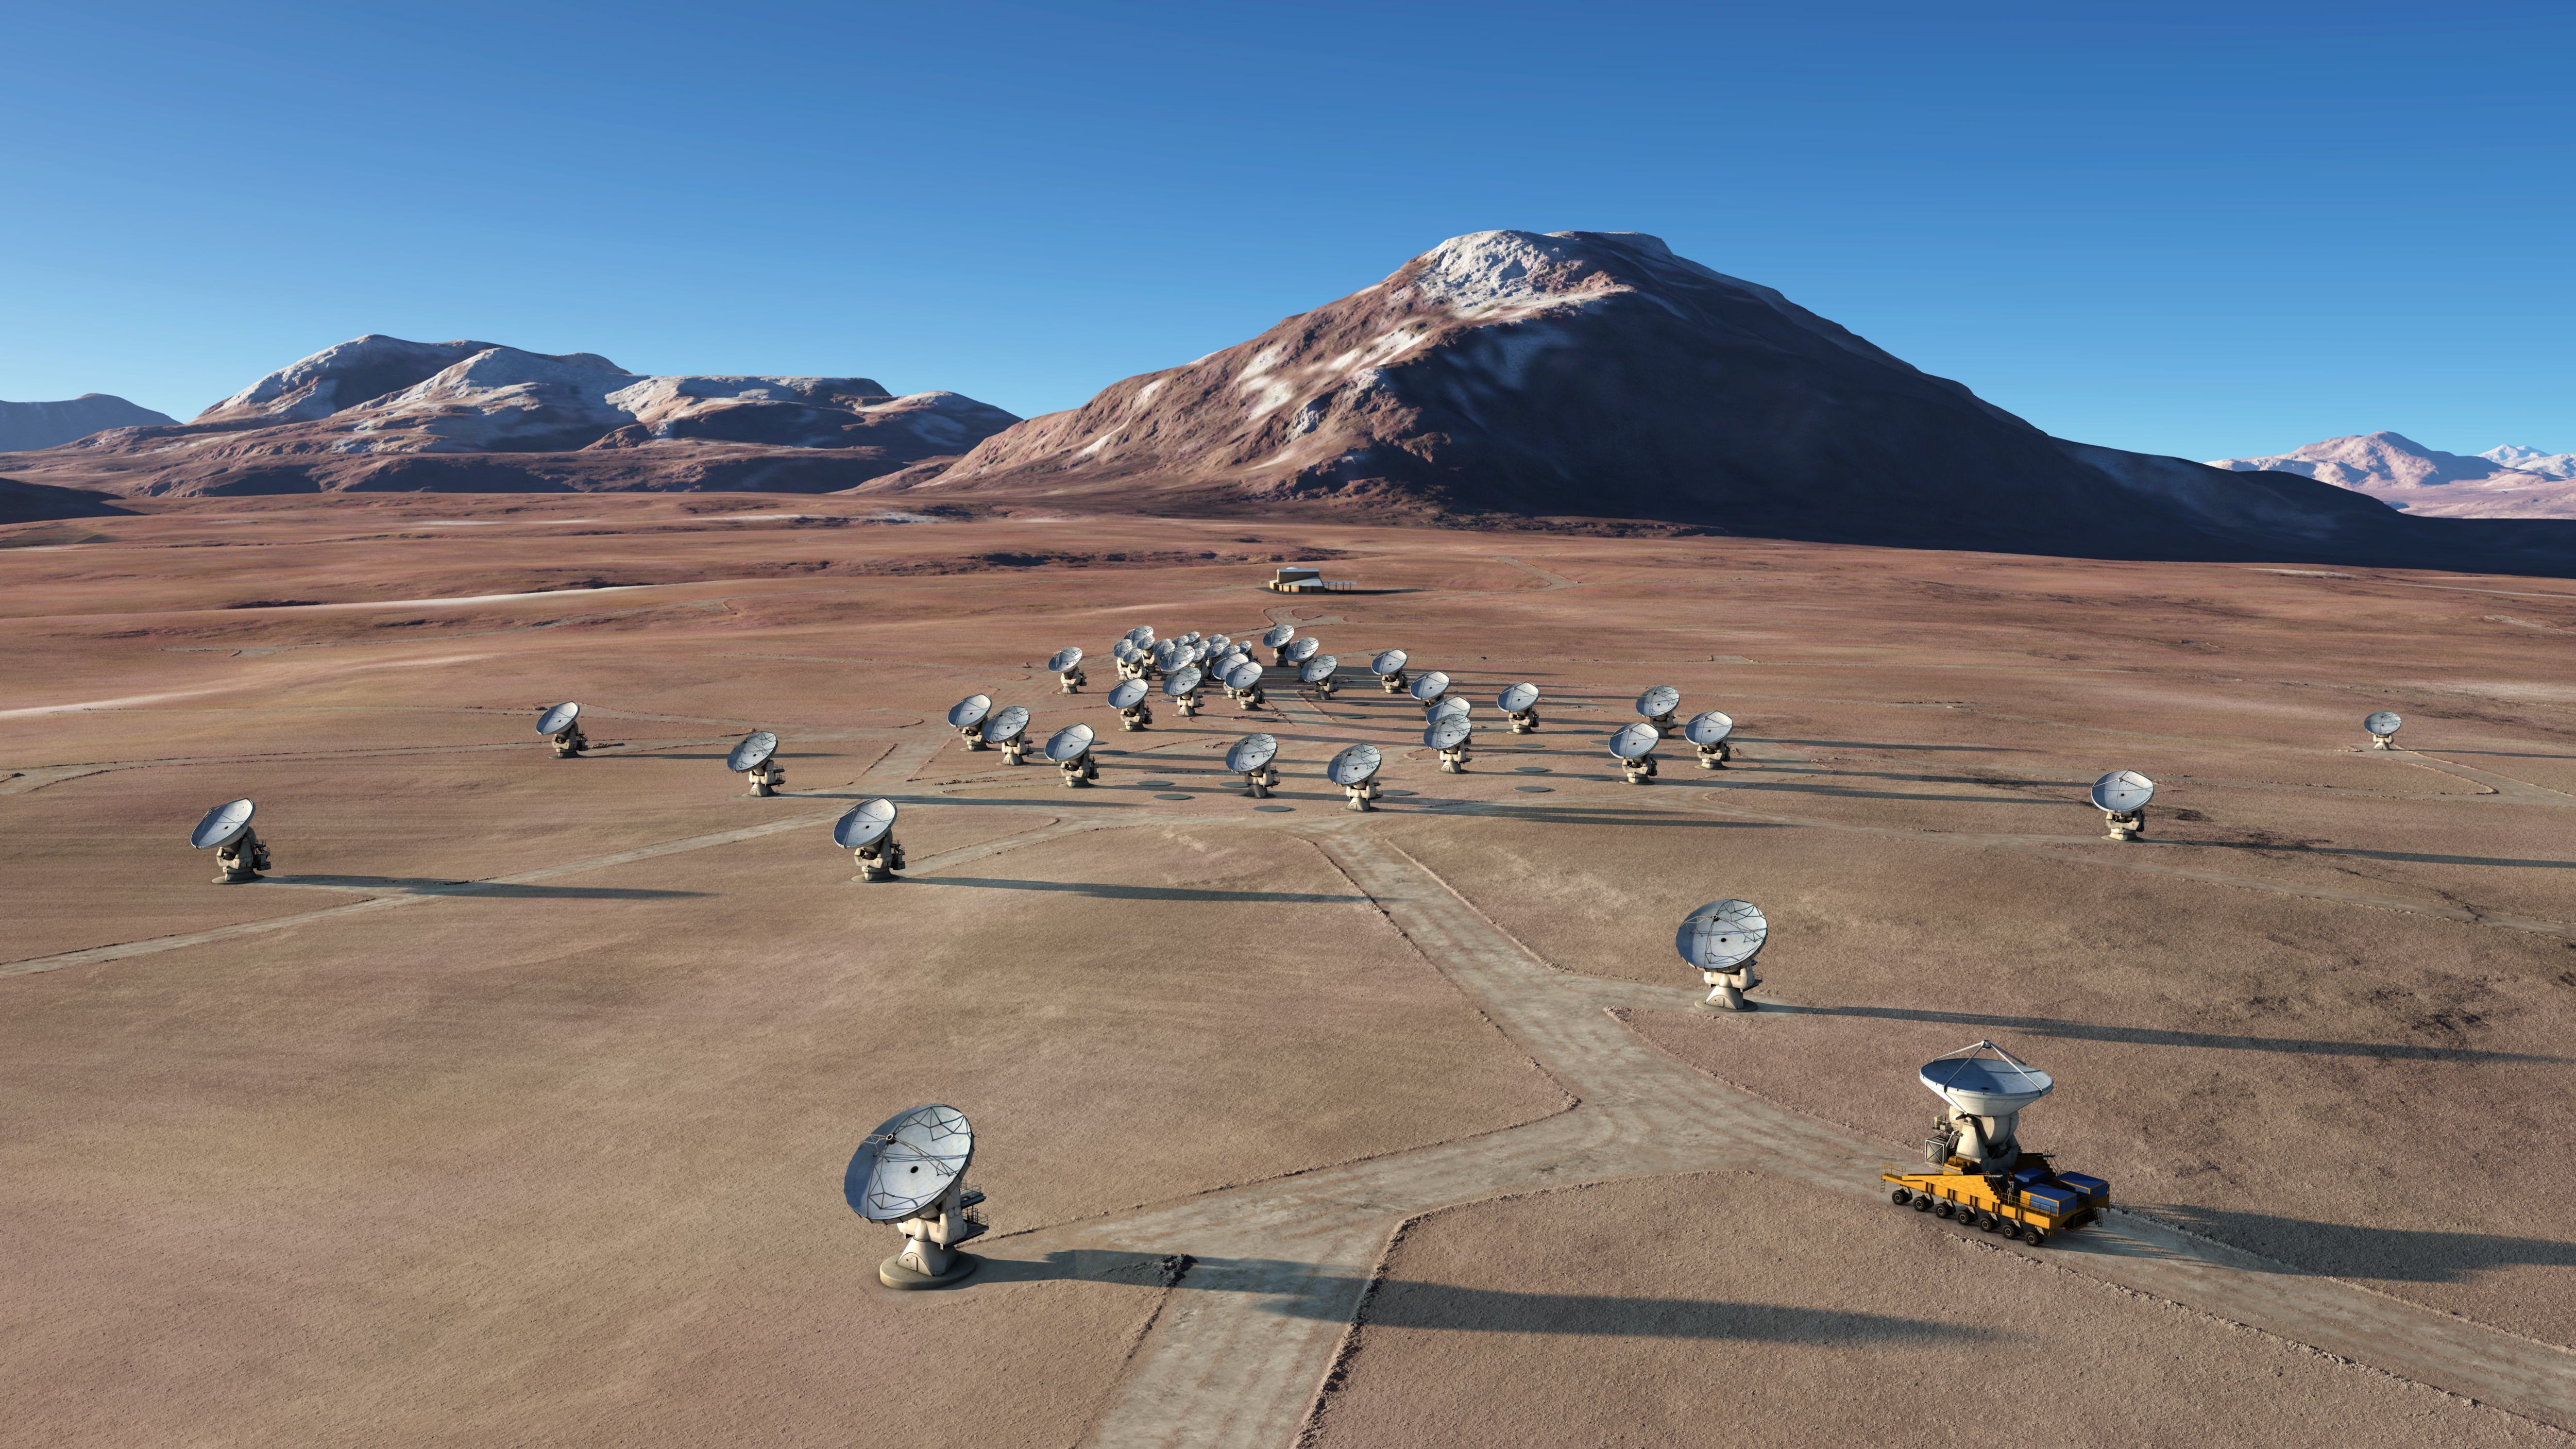
\includegraphics[width=\linewidth]{ALMA_universetoday.jpg}
%   \captionof{figure}{A rendering of ALMA. Antennae may be moved using a large truck, as seen in the lower right corner.}
%   \label{fig:test1}
% \end{minipage}%
% \begin{minipage}{.27\textwidth}
%   \centering
%   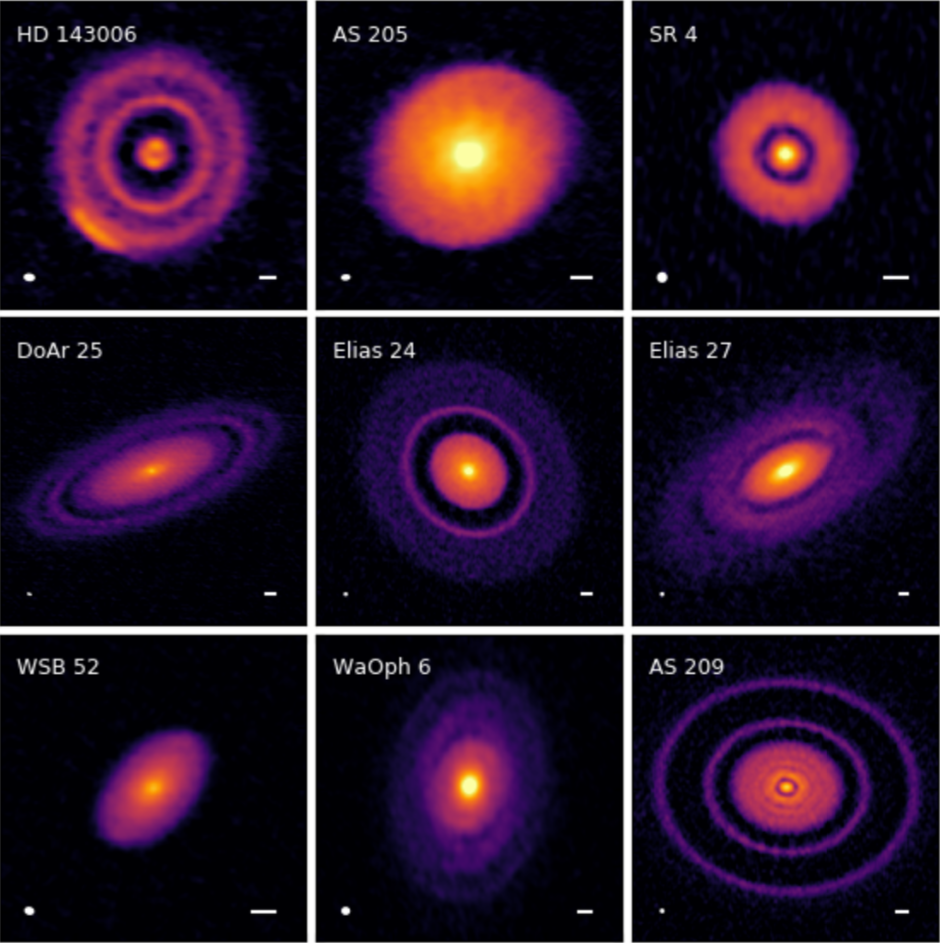
\includegraphics[width=\linewidth]{Andrews2018_proplyds.png}
%   \captionof{figure}{Impressive images of disks from Andres et al (2018)}
%   \label{fig:test2}
% \end{minipage}
% \end{figure}




\subsection{Continuum Emission}
\label{section:continuum_emission}

Continuum emission observations integrate flux from a wide band of frequencies, just as our eyes do in the optical. They are appealing for their simplicity and because, by integrating a wide band, they are sensitive to faint objects.

When observing protoplanetary disks, an understanding of planet formation is often a guiding motivation. One parameter that is critical to the planet-forming process is total disk mass. We know that, to first order, when a disk is optically thin, its total mass, $M_{\text{disk}}$, is linearly proportional to its flux density, $F_{\nu}$ \citep{Hildebrand1983}, which is found from an observation of continuum emission. This relationship is given by

\begin{align}
M_{\text{dust}} = \frac{F_{\nu} d^2}{\kappa_{\nu}\ B_{\nu}(T_c)},
\end{align}

%below: really opacity power law index, but simpler this way and they mean the same thing.
where $d$ is the source's distance, $\kappa_{\nu}$ is an assumed dust opacity, and $B_{\nu}(T_c)$ is the Planck function at a given charatcteristic temperature, $T_c$. The value of $T_c$ and disk opacity can be inferred without much difficulty by fitting the disk's SED using a simple model. This function is, of course, rather approximate; it assumes a single temperature and single dust opacity (a function of composition and grain size distributions) throughout the disk. The assumption of optically thin emission means that calculations made will inherently be lower limits, since any substantial optical depth will block emission from inner regions of the disk. Futhermore, even in the case of optically thin emission, significant mass may be locked up in bodies that are invisible to our observations.

Traditionally, studies have used observed continuum fluxes to estimate dust mass and then inferred a total gas mass by assuming a 100:1 gas/dust ratio, based on the ratio observed in warm ISM clouds. However, an ALMA survey of 89 disks in Lupus tracing both continuum emission and two CO isotopologues \citep{Miotello2016,Miotello2017} found the true value of this value to be highly variable, often falling closer to 10 (Fig \ref{fig:gas-dust-ratios}), and \citet{Liu2018} found that a ratio of 100 provoked instability (as measured by the Toomre criterion) in their smoothed-particle hydrodynamic simulation of the MWC 480 disk; instead, they found that values of 6-12 yielded their best results. \textit{Could cite Bergin+ 2013 here for coming up with the HD stuff, but not sure how to make it work narratively.} In short, this ratio introduces a significant source of uncertainty, possibly of up to two orders of magnitude, into existing calculations of gas mass in protoplanetary disks based that are based on continuum emission.



\begin{figure}
\centering
  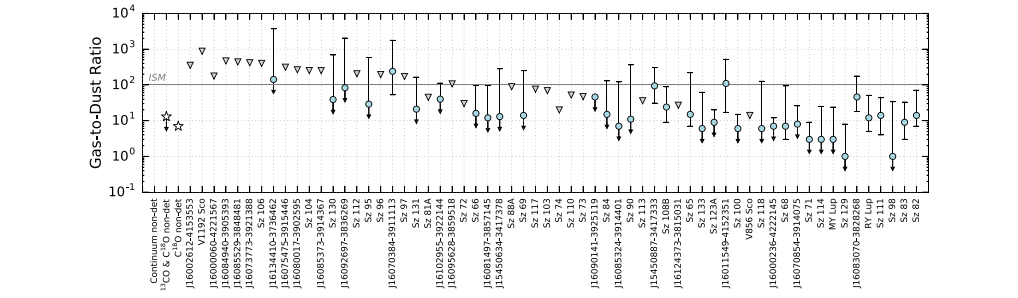
\includegraphics[width=\linewidth]{gas-dust-ratios_Miotello16.png}
  % 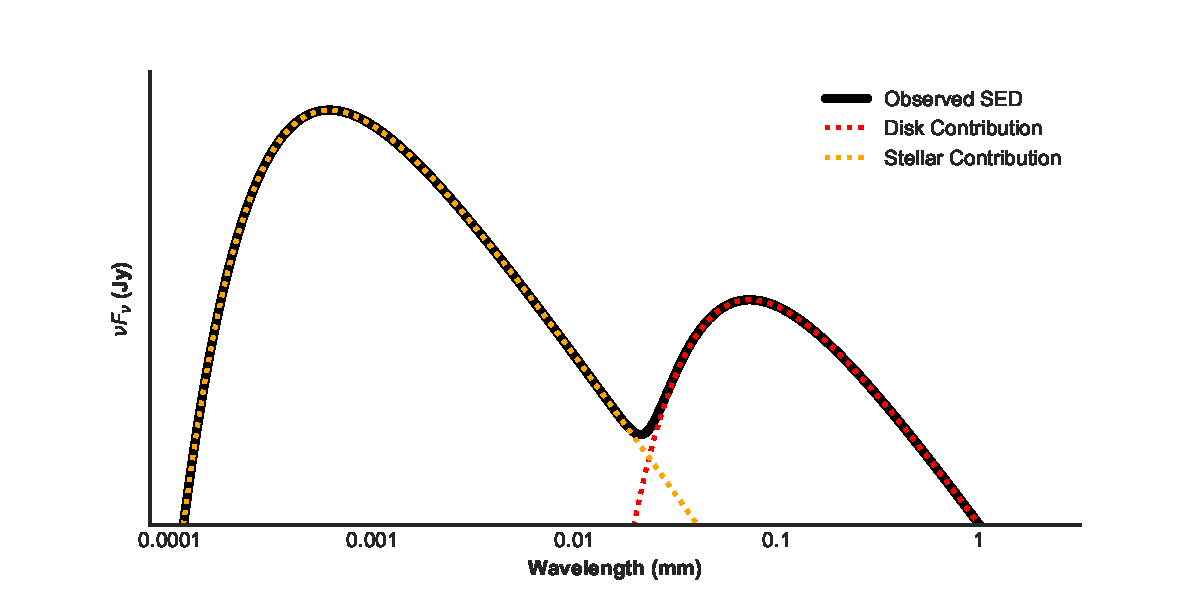
\includegraphics[width=\linewidth]{example_SED.pdf}
  \captionof{figure}{Gas-to-dust ratios in protoplanetary disks in Lupus \citep{Miotello2016}. The ratio is highly variable and rarely best described by the canonical value of 100:1. Blue points indicate detections, and gray triangles indicate upper limits. Error bars with downward arrows indicate sources detected in $^{13}$CO but not C$^{18}$O, for which the authors did not establish lower mass limits.}
  \label{fig:gas-dust-ratios}
\end{figure}







\subsection{Line Emission}

As molecules collide with one another or absorb light, they gain energy, entering higher rotational energy states. However, as their presence in these states cannot be sustained without the addition of more energy, they will de-excite soon after. This de-excitation process - stepping down from one rotational energy state to the one below - causes the emission of light. Every transition in every molecule emits at its own specific frequency, or rest frequency, making that light identifiable to observers. We may observe a specific rotational transition from a single type of molecule by tuning our receiver to be sensitive to a very narrow window of frequencies immediately around the rest frequency of the transition of interest. This is known as a spectral window. The narrow range of frequencies at which a given molecular transtion emits makes ALMA's large sensitivity particularly crucial for observations of molecular lines at high spectral resolution or in rare species.

One immediate feature that line emission gives us access to is velocity information: since all emission should have a single frequency (the transition's rest frequency), we immediately know that any variation from that central frequency is a result of Doppler shifting caused by line-of-sight velocity\footnote{Technically, the uncertainty principle tells us that a line will have some ``natural" width, but this width is small compared to the Doppler width.}. This allows us to make a ``moment-one" map of emisison, which shows the intensity-weighted velocity structure of the disks (Fig \ref{fig:ex_mom1}).


\begin{figure} %[t!]
\centering
  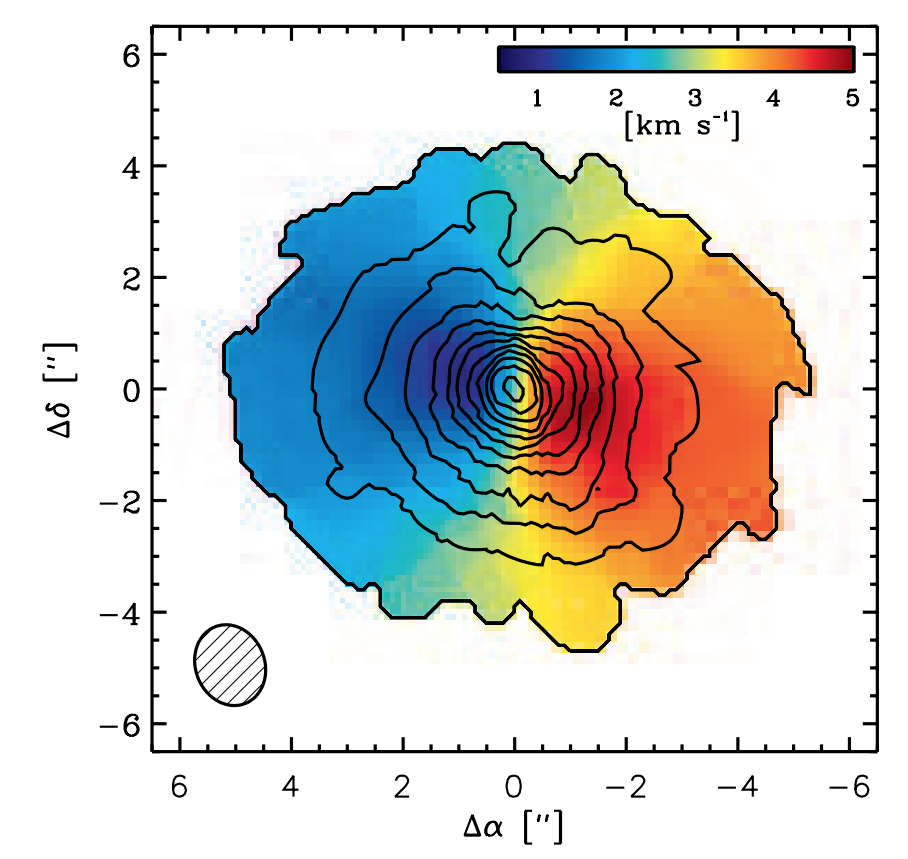
\includegraphics[width=\linewidth]{example_m1_image.png}
  \caption{An example of a moment-one map of a protoplanetary disk, drawn from \citet{Rosenfeld2012}. Colors correspond to intensity-weighted velocity; in other words, how quickly material is moving relative to the observer. One may consider this analogously to a spinning Frisbee, approaching the reader edge-on, where one half of the disk is spinning outwards (away from us) as the other side approaches. From this image, we immediately gain several pieces of information: for example, in this case, the disk as a whole is receding from view (since the velocity's "zero point", in yellow/green, is moving at 3 km/s), and that the disk's eastern half is spinning away from us, while the western half comes towards us. This gives us a quick understanding of the disk's kinematics.}
  \label{fig:ex_mom1}
\end{figure}


% Ignoring this from Meredith: (or multiple isotopologues, ideally, but we don’t have that in this case)
Observations of line emission also give us information about both the temperature and density structures of the disk, since these are the two factors that influence how much emission we observe. However, in the case of optically thin emission, the two are degenerate, since an increase in either one will increase emission intensity. In this case, we may combine observations of multiple species to model the temperature structure of a disk. In the case of an optically thick line, however, the temperature and density are no longer degenerate, since all emission originates from the $\tau=1$ surface, which removes density from the equation and gives us a value for the temperature at that point in the disk's vertical structure. This is valuable, since the a disk's vertical temperature profile varies significantly, with the surface notably warmer than the midplane.

Besides offering information about radial density and temperature profiles, line emission also provides another way of finding total disk mass. Like the initial cloud that the star and disk formed from, the vast majority of the disk's mass comes in its gas, and like that initial cloud, the vast majority of that gas is molecular hydrogen, or H$_2$. However, since H$_2$ is a symmetric molecule and thus has no permanent dipole moment, it has no rotational transitions and does not emit in the radio, making it invisible to our instruments. As a consequence, we must instead observe emission from other molecules, make assumptions about those molecules' abundances relative to H$_2$, and extrapolate the total disk mass.


To do so, one generally begins with CO, second most abundant molecule behind H$_2$. Thanks to its abundance, as well as its relatively low excitation temperature, CO provides robust, bright emission. Drawing on measurements of CO/H$_2$ ratios in warm dense cloud \citep{AikawaHerbst2003,Fogel2011}, we use a ratio of 1:10000, or 10$^{-4}$, to represent CO's relative abundance in protoplanetary disks, while for other, more complex molecules, relative abundances are generally drawn the interstellar-medium literature and chemical modeling.

However, this CO/H$_2$ ratio of 10$^{-4}$, which is frequently used to calculate total disk gas masses \cmmnt{(e.g. \citet{Ansdell2017})} comes with significant uncertainty. Using a gas-grain chemical model \citet{Reboussin2015} showed, through an analsysis of CO isotopologues, that at low temperatures (below 30-35K), CO is converted to less volatile molecules (typically s-CO$_2$ or s-CH$_4$). This means that below these temperatures, relative CO abundance quickly falls about two magnitudes below the literature value of 10$^{-4}$. \citet{Schwarz2016} followed this modeling with high spectrospatial resolution ALMA observations of four CO isotopologues in the nearby protoplanetary disk TW Hya, and confirming a ratio of C/H$_2 = 10^{-6}$. Additionally, \cite{Yu2017} notes that CO depletion in the outer disk and optically thick emission from the inner disk has lead observers (e.g. \citet{Ansdell2017}, who found surprisingly low disk masses in their survey of ONC proplyds) to underestimate disk mass by more than an order of magnitude if they assume CO/H$_2 = 10^{-4}$ and optically thin emission. They and \cite{Cleeves2015} also note that CO abundances change on short ($\sim$ 1 Myr) timescales, resulting in a degeneracy between disk age and mass. Ultimately, CO's tight dependence on disk temperature and its evolutionary trends with age increase the need for a well modeled temperature profiles to inform the selection of an appropriate molecular abundance of CO.



\section{Disks \& The Role of Environment}


%REWORK: This is a rough transition from that CO talk.

There is significant evidence that most stars in our galaxy \citep{LadaLada2003,Mann2015}, including our own Sun \citep{Gaidos2009,Tachibana2006}, formed in high-mass star forming regions, or HMSFRs. Therefore, understanding our own creation story necessitates the understanding of protoplanetary disk evolution in these SFRs, and the role that environment plays in that process. However, until ALMA came online in 2012, line-emission studies of disks in these HMSFRs were not feasible, due to the need for increased sensitivity and resolution in the observations.

Now that this telescope is available, however, HMSFRs are open for observation. We may use this opportunity to try to better understand the role that environment plays in the development and evolution of protoplanetary disks, comparing them to the well-studied disk population in low-mass \citep{AndrewsWilliams2005,Mann2015} and the one well-characterized disk in an HMSFR \citep{Factor2017}, and evaluate how that environment may affect planet-formation potential.

% Charles/Elizabeth Lada for star formation in HMSFRs
% Star formation reviews; check Protostars and Planets VI


\subsection{The Minimum Mass (Extra-)Solar Nebula}

The minimum-mass solar nebula (MMSN) is a conceptual aid used to inform astronomers about the distribution of material required to form a planetary system \citep{Weidenschilling1977}. The MMSN is the radial mass profile that our own Solar System would present if the mass of each planet were, rather than being bound up in spheres, instead ground up and spread across the ring bound by the orbits of their inferior and superior neighbors. Gas is then added to the ring until the its gas:dust ratio reaches the canonical interstellar-medium value of 100:1\footnote{This ratio is discussed more in \S\ref{subsection:continuum}} (meaning that gas giants like Jupiter would have very little gas mass added, while terrestrial planets like Earth would have their mass significantly increased). The resulting mass profile represents the minimum surface density required to form our own protoplanetary disk and thus a way to inform our comparisons of other disks to our own. When this surface density profile is integrated into a single mass, it gives $M_\text{MMSN} = 0.01 M_{\odot}$.

It is, of course, an extremely approximate characterization. One significant assumption it makes is that our planets formed in their current positions. This is a statement that we know both to be false \citep{Walsh2011,Tsiganis2005} and consequential, since planetary migration can cause disks to lose mass by pushing competing planetesimals either out of orbit or into inner regions of the disk where they may be more susceptible to accreting onto the host star. Another assumption being made is that the chemistry is radially and temporally constant, which is also known to not be the case \citep{vanDishoeckBlake1998}.

The MMSN model was generalized to be tolerant to a wider diversity of planetary systems by \citet{Kuchner2004} as the minimum-mass extrasolar nebula (MMEN), using 26 Doppler-detected planets in multi-planet systems to construct a disk analogous to that of the MMSN. \citet{ChiangLaughlin2013} developed a similar model, this time drawing on Kepler and HARPS planets ($n \approx 10^5$) to explain the existence of close-in ($P < 100$ days) super Earths, which make up approximately half of the planets observed in those catalogues. Both models assume that planets formed at or near their current positions. However, \citet{Raymond2014} showed, using 191 multi-planet systems primarily drawn from the Kepler catalogue, that the resulting range of surface density profiles was broad, and thus that using a single, ``universal" profile to locate disks with planet-forming potential - as the MMSN/MMEN purports to offer - was not plausible. They note that this broad spread likely reflected the necessity for consideration of planet migration, particularly amongst gas giants.

Still, while the MMSN clearly makes significant assumptions that lead to inconsistencies, it is nonetheless used as an approximate barometer for planet-forming potential.




\subsection{Low- and High-Mass Star Forming Regions}
Thanks to limitations in sensitivity and resolution, most submillimeter surveys in the pre-ALMA epoch focused on young disks in the nearby low-mass SFRs of Taurus-Auriga and $\rho$ Ophiuchus. Dust-emission studies of disks in this regions by \citet{AndrewsWilliams2005,AndrewsWilliams2007} have yielded a wide range of disk masses, with a median of 0.005 M$_{\odot}$ and a significant fraction with mass greater than the MMSN. This large fraction of disks with planet-forming potential is consistent with what we would expect based on the enormous - and still growing - number of exoplanets that have been discovered in the last two decades.


Of course, studying only nearby disks paints an incomplete picture of the population and its evolutionary trends; for one, most stars form in high-mass SFRs \citep{LadaLada2003,Mann2015}, and low-mass SFRs are qualitatively different than their high-mass siblings. High-mass SFRs are massive, dense clusters with large abundances of high-mass O and B stars. Protoplanetary disks in these regions experience accelerated mass loss, thanks to the powerful ionizing radiation from the high-mass stars \citep{Anderson2013,Kalyaan2015,Xiao2018}. This mass loss is likely a problem for planet formation \citep{Johnstone1998,Ovelar2012} and negatively affects potential habitability \citep{Kruijssen2019}, but its effects are not yet well understood. It is because of these factors that we would like to study disks in high-mass SFRs.


\begin{figure}[t!]
\centering
  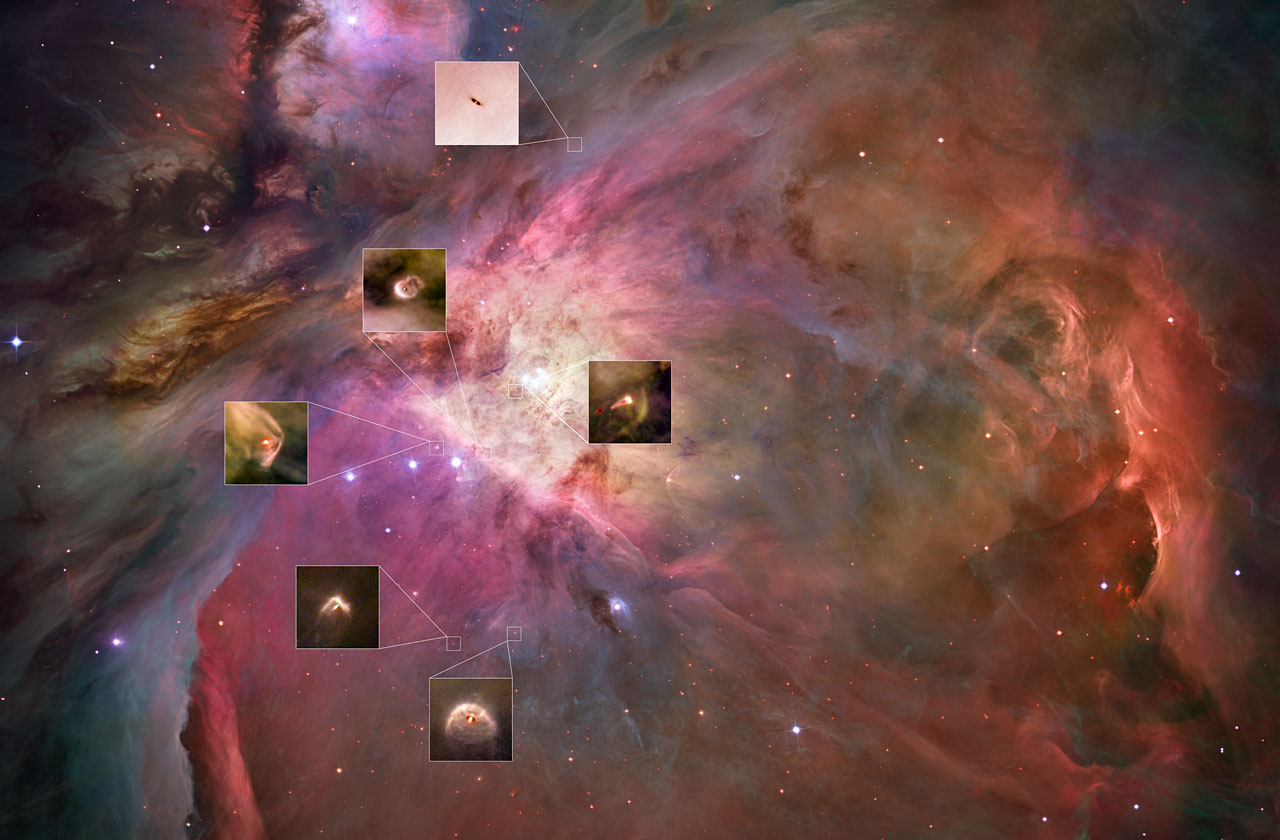
\includegraphics[width=\linewidth]{HST_Orion_proplyds.jpg}
  \captionof{figure}{Proplyds in the Orion Nebula. The closer a proplyd is to a large, bright star, the more visibly windswept it is. Image courtesy of the Hubble Space Telescope Treasury Program on the Orion Nebula (\cite{Robberto2013})}
  \label{fig:HST_ONC}
\end{figure}



The nearest high-mass SFR to us is the Orion Nebula Cluster (ONC), 389 pc away. The Hubble Space Telescope was the first to dedicate significant time to the ONC, producing an abundance of iconic and awe-inspiring images the cluster and of the disks it hosts \citep{Ricci2008}. These studies have guided many subsequent observations, including many in the radio. Many of the cluster's protoplanetary disks (or proplyds, as those in the ONC are called) are visibly teardrop-shaped, tailing away from the cluster's biggest and brightest stars, which are pushing a four parsec-diameter bubble outward at 13 \kms \citep{Pabst2019}. Images like Fig \ref{fig:HST_ONC}, showing disks being pushed away from nearby bright stars, and countless others demonstrate the harsh environment that these young disks exist in. Indeed, the influence of these large stars has already been demonstrated, both in their affect on mass-loss rate and mass distribution. Statistically-significant anti-correlations between disk mass and proximity to the ONC's central O star, $\theta^1$ Ori C, have been shown using both data from the SMA \citep{MannWilliams2009} and ALMA \citep{Mann2014,Ansdell2017,Eisner2018}.


Furthermore, both observations \citep{HenneyODell1999} and modeling \citep{Haworth2016} characterizing mass-loss rates for these proplyds in the Orion Nebula have found rates of $\dot{M} \approx 10^{-7}-10^{-5}$ M$_{\odot}$ yr$^{-1}$, implying that a typical disk (i.e. one of MMSN-scale, or $\sim0.01$ M$_{\odot}$) should be fully dispersed before giant planets could form \citep{Hubickyj2005} and before they could reach the inferred age of the disk-hosting stars in the ONC of $\approx$ 2 Myr \citep{Reggiani2011}.

% $''$There are probably more recent references for all of these.  Did you know that you can do a backwards citation search in ADS, and see which papers cited a paper of interest?  If it’s a paper with a ton of citations (as many of these are) it can be tough to sort through the results, but reading the titles can help, and then looking at the introductions of the most recent papers to see which other papers they cite. $''$ REWORK

 
Despite all this, not only do we still see disks, but we still see significant planet-forming potential in the Orion Nebula, potential that is comparable to that of other low-mass SFRs. A full 30\% of disks surveyed in the ONC have disks with masses greater than or equal to the MMSN \citep{Mann2014}, falling comfortably between $\rho$ Ophiuchus' 29\% \cite{AndrewsWilliams2005} and Taurus' 37\% \citep{AndrewsWilliams2007}.


However, since all these surveys are based exclusively on the analysis of dust continuum emission, the comparison is profoundly hamstrung by its reliance on assumptions of gas/dust ratios drawn from the ISM literature. This means that the resulting understanding of the gas masses in these regions is directly proportional to that 100:1 gas/dust ratio, a value that is almost certainly not accurate (as discussed in \S\ref{chap:continuum}). The consequences of this assumption are signficant, since a disk's gas mass directly determines its giant planet forming potential both by setting the amount of raw material available to the forming planet as well as by influencing the environment's turbulence profile and planets' migratory patterns within the disk. Furthermore, these continuum surveys cannot reveal these disks' chemistries and the environmental influences that likely affect them, instead simply assuming solar composition. Together, these assumptions regarding both the total gass mass as well as its composition result in a heavy asterisk accompanying any claims we make about the birth and evolution of protoplanetary disks in high-mass SFRs. To solve this, we must understand the chemical make up of these disks, and for that we need studies of line emission.




\citet{Mann2014} made the first line-emission survey of the Orion proplyds as part of ALMA's Cycle 0 Early Science operation. The survey studied 22 disks in four molecular lines (HCO$^+$, HCN, CO, and CS) and $856 \mu$m continuum, and calculated each disk's dust mass from the continuum emission. Since then, only one of the disks has had its line data analyzed. \cite{Factor2017} performed an analysis of the radial distribution of one of the disks' gas by modeling emission from the lines to try to understand the chemical abundance and physical structure of different molecules in the disk. This fitting process was performed on three of the four molecular lines (as CS had insufficient signal to produce meaningful constraints).

In the study, the authors found several unexpected features: their measurement of the disk's HCN abundance was higher than expected (although HCO$^+$ and CO abundances were consistent with literature values from low-mass SFRs), their mass measurement for the central star was inconsistent with the previously-determinded spectral type, and they found a spatially unresolved high-velocity excess emission feature in the HCO$^+$(4-3) and CO(3-2) lines, with a positional offset from the central star. For this emission feature, they found that the source was blue shifted by $-6.2$ km s$^{-1}$ relative to the systemic velocity, had a position consistent with a $60\pm20$ AU Keplerian orbit, and had an inferred H$_2$ mass of 1.8-8 M$_\text{Jup}$. They determined that the excess of emission was caused by a local density and/or temperature fluctuation in the inner disk, indicating that it was not a jet or cloud contamination. The authors propose that this could be the result of young Mars-sized bodies, collisions between particles trapped in mean motion resonance by a giant planet, magnetic-field-induced zonal flows, or planet formation.


These unexpected results demonstrate the need for further analysis of disks in this survey. The binary system that is the subject of this thesis is drawn from the same survey, representing the second and third ONC proplyds to have their temperature and density profiles characterized.





\section{d253-1536: A Misalgined Binary System}

The subject of this thesis is the system d253-1536, a binary of pre-main sequence stars in the M43 region of the Orion Nebula Cluster. Each star has its own proplyd. The stars' projected separation is somewhat atypically wide (approximately 428 au), and their rotational axes are misaligned. Each star in the system has its own disk, henceforth called disk A and disk B (east and west, respectively, in all images of the system\footnote{The reader will recall that this corresponds to disk A being on the left and disk B on the right of all images, since east and west are inverted in celestial coordinates relative to our familiar geographic ones.}).

\subsection{Local Environment \& Features}
Many previous surveys have studied disks in the famous M42, or Orion Nebula, which lies adjacent to M43, and particularly the Trapezium cluster, a region near M42's brightest star O-star $\theta^1$ Ori C. \citet{Mann2014} found a statistically significant correlation between disk mass and distance from $\theta^1$ Ori C in a study of 70 proplyds (Fig. \ref{fig:onc_disk_relations}), particularly within 0.03 pc of the star, where there is a lack of disks more massive than $3 M_\text{jup}$. These disks are also truncated in radial extent, with no disks extending out past 60 AU in this region \citep{Eisner2018}.


\begin{figure}[htp]
  \hspace*{\fill}%
  \subcaptionbox{\label{fig:onc_disk_masses}}{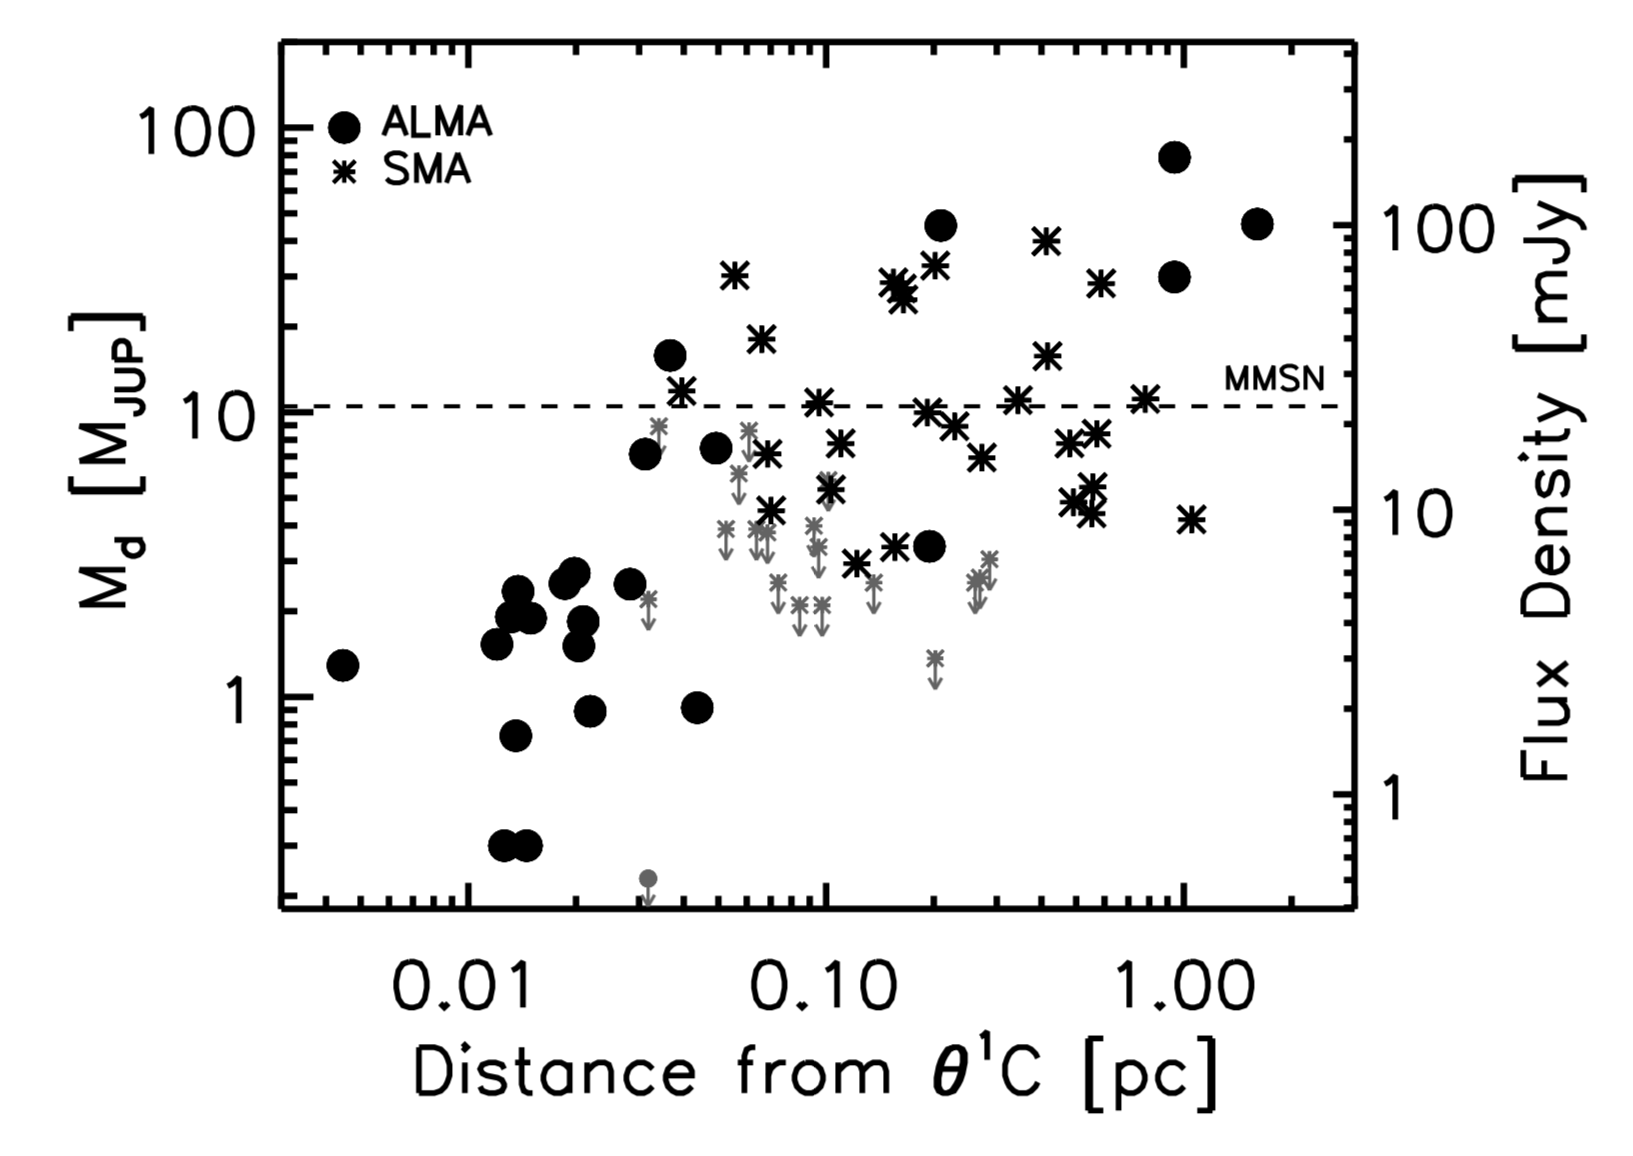
\includegraphics[width=0.52\linewidth]{onc_disk_masses.png}}\hfill%
  \subcaptionbox{\label{fig:onc_disk_radii}}{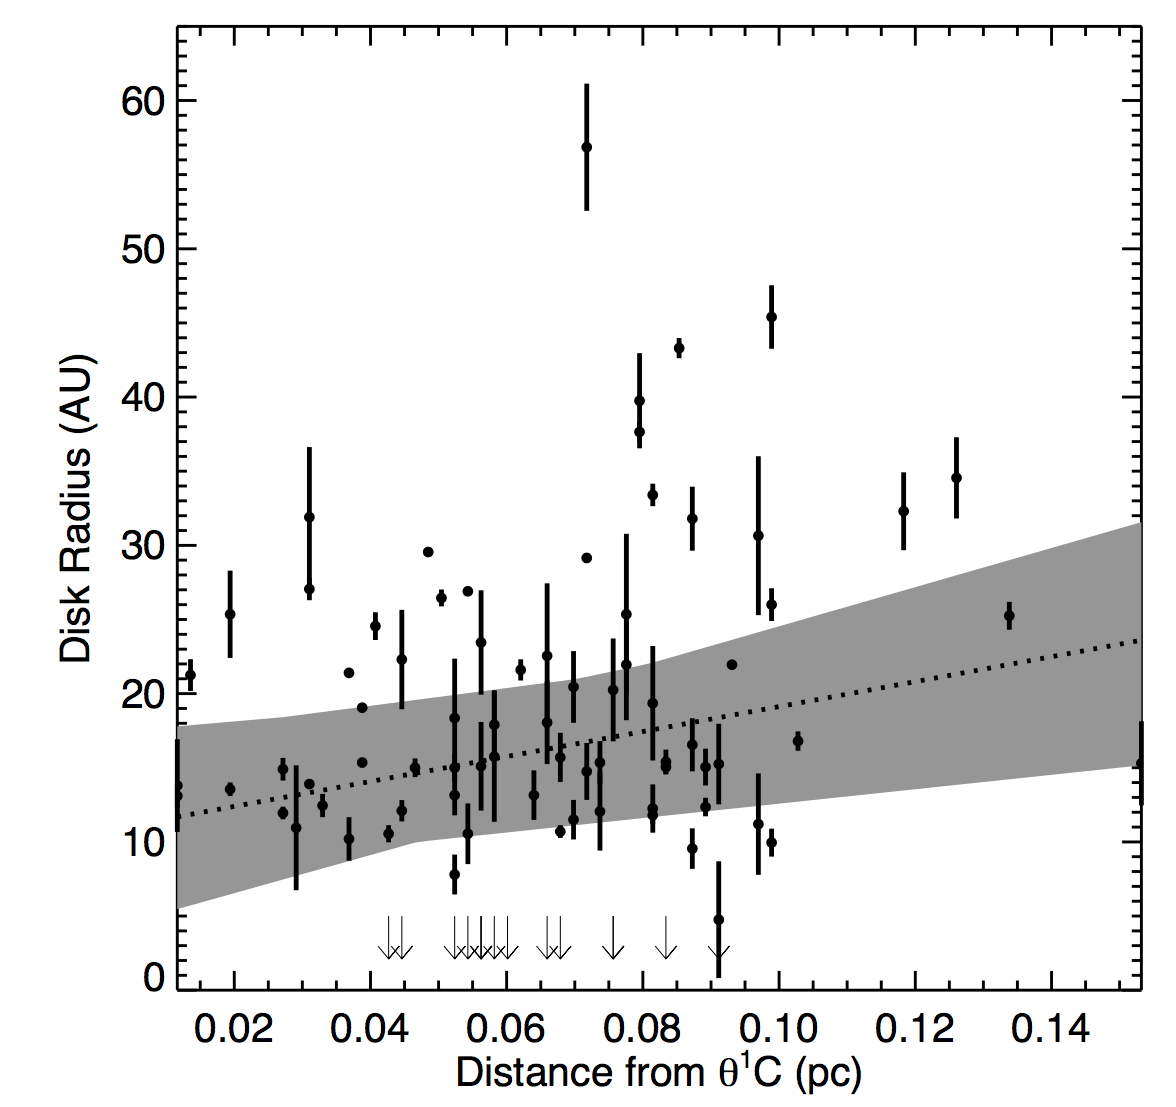
\includegraphics[width=0.38\linewidth]{onc_disk_radii.png}}%
  \hspace*{\fill}%
  \captionof{figure}{\textit{Left}: The masses of 70 ONC proplyds are plotted against their projected distance from the Orion Nebula's central O-star, $\theta^1$ Ori C, drawn from surveys from ALMA and the SMA \citep{Mann2014}. Grey markers indicate $3 \sigma$ upper limits for non-detections. The dashed line at 10 M$_\text{Jup}$ indicates the minimum-mass solar nebula. As is clear from this plot, a statistically-significant correlation was found between disk mass and distance from $\theta^1$ Ori C. \textit{Right}: Radius is also affected by proximity to $\theta^1$ Ori C \citep{Eisner2018}}
  \label{fig:onc_disk_relations}
\end{figure}


However, because of M43's separation from the Trapezium cluster (it lies $\geq$ 1 pc to the cluster's north; see Fig.\ref{onc_map}), disks in this region do not experience the same levels of photoevaporation. M43 has only one large emitter, NU Ori, which is a triple-star system whose main component is a B-stype star. d253-1536 is wrapped in an ionization bow shock, HH 668 A (Fig.\ref{fig:v2434ori_smith05}), about 1" to the system's west and facing towards NU Ori, but otherwise the system shows no signs of influence from giant stars, whether in photoevaporation or in morphological influences \citep{MannWilliams2009}.

The misalignment of the disks' rotational axes is fairly typical of wide binaries like this one \citep{Williams2014}. The frequency with which these wide binaries present such misalignment indicates that wide binaries likely do not form in large, co-rotating structures, and emphasizes the importance of gas turbulence and inter-stellar interactions for young stars.


The system's larger disk, disk A, has a large jet emanating from it in observations in the optical made with HST \citep{Smith2005}. However, since the jet is not visibile in the radio, we make no attempt to discuess, model or explain it.


\begin{figure}[t]
\centering
  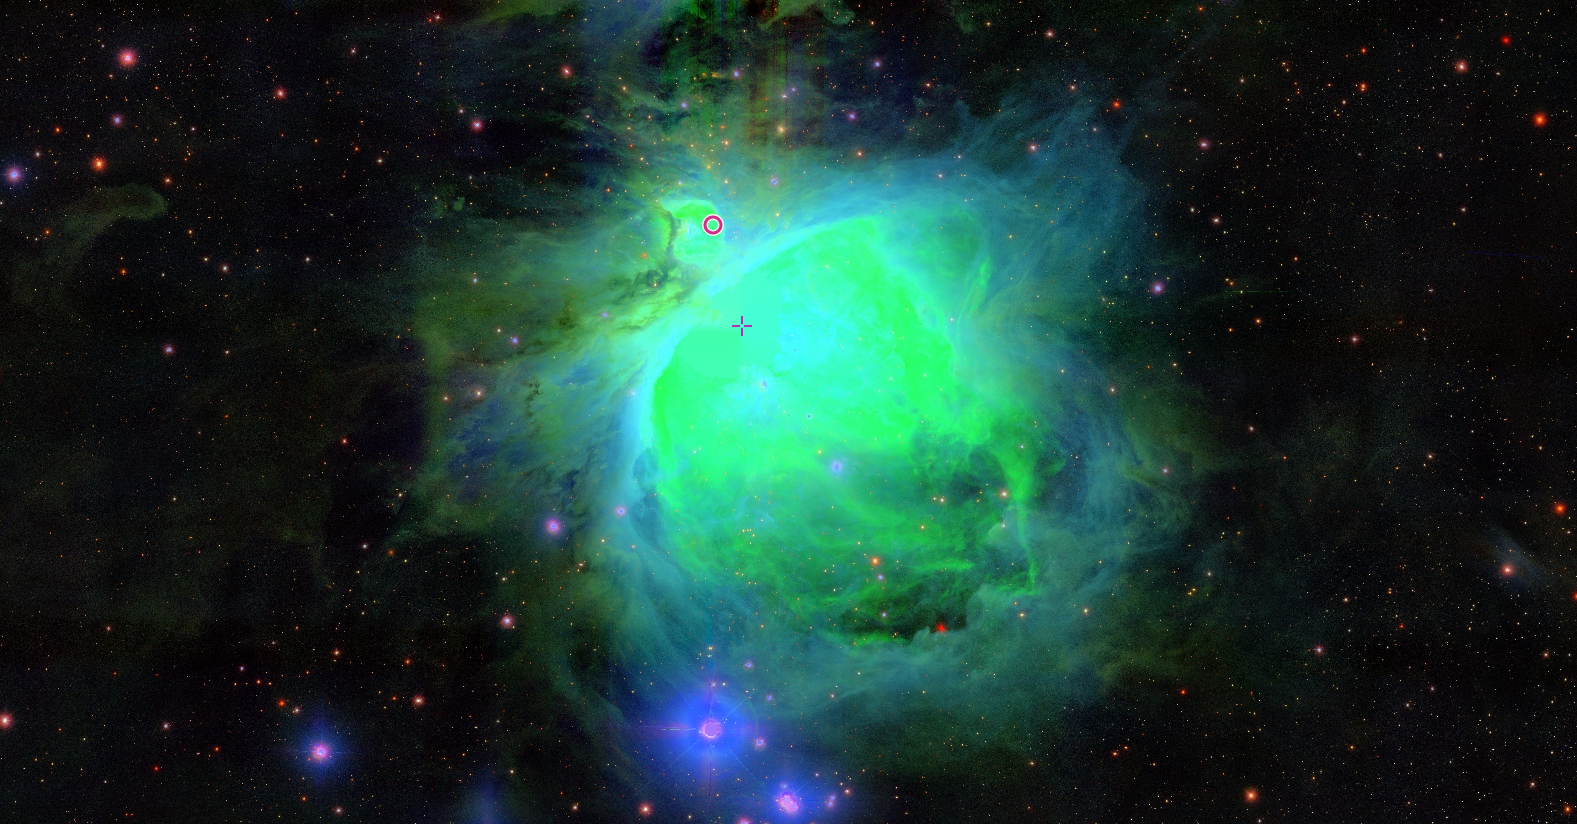
\includegraphics[width=\linewidth]{ONC_Map.png}
  \caption{M42 and M43, shown in SDSS coloring, with the locations of d253-1536 (marked with a red circle) and $\theta^1$ Ori C (marked with crosshairs), the heart of the Trapezium cluster. Map created in AladinLite viewer. Because of the large separation between d253-1536 and Trapezium, the disks don't show the same obvious marks of influence from OB stars seen in other disks closer to the heart of M42.}
  \label{fig:onc_map}
\end{figure}
%
% \begin{figure}[t!]
% \centering
%   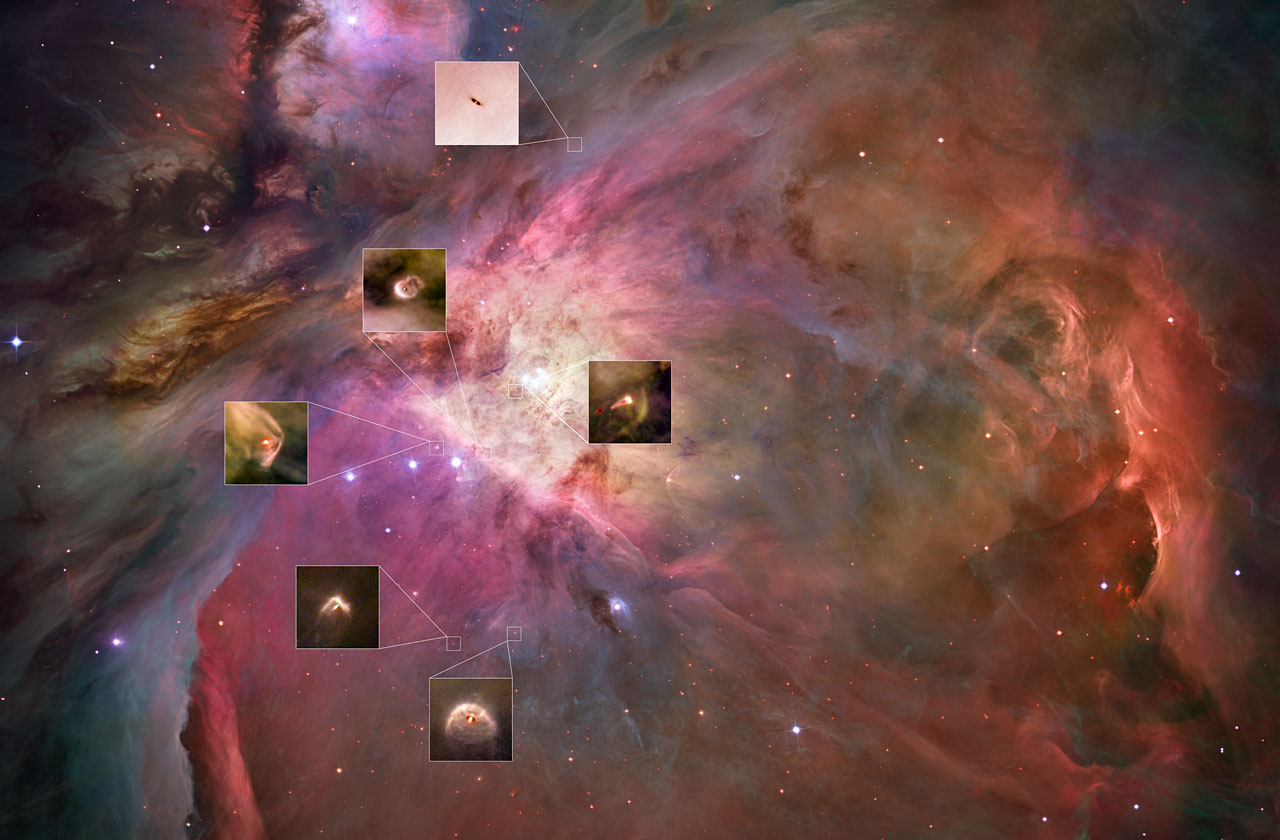
\includegraphics[width=\linewidth]{HST_Orion_proplyds.jpg}
%   \captionof{figure}{Proplyds in the Orion Nebula. The closer a proplyd is to a large, bright star, the more visibly windswept it is. Image courtesy of the Hubble Space Telescope Treasury Program on the Orion Nebula (\cite{Robberto2013})}
%   \label{fig:HST_ONC}
% \end{figure}




\subsection{Previous Observations}

\begin{figure}[htp]
  \hspace*{\fill}%
  \subcaptionbox{\label{fig:v2434ori_smith05}}{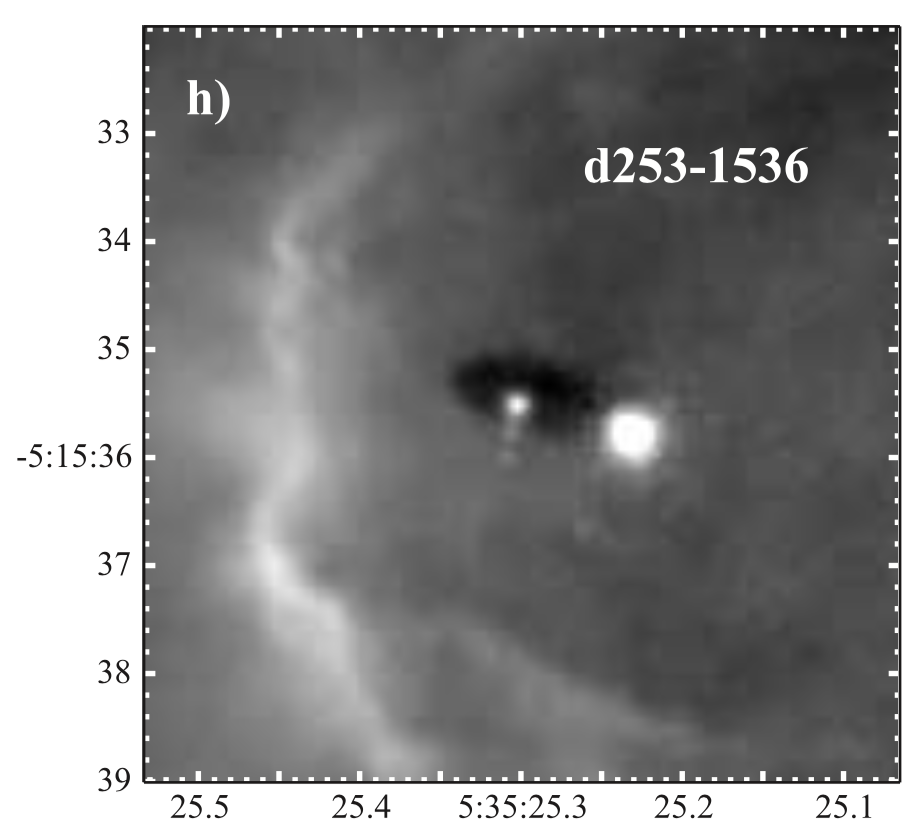
\includegraphics[width=0.33\linewidth]{V2434Ori_Smith05-2.png}}\hfill%
  \subcaptionbox{\label{fig:v2434ori_mann09}}{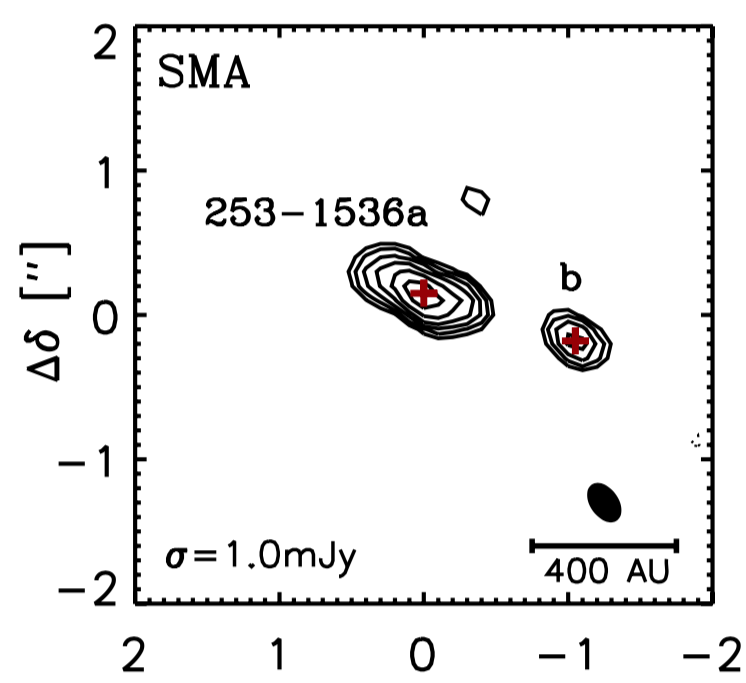
\includegraphics[width=0.33\linewidth]{V2434Ori_Mann09.png}}\hfill%
  \subcaptionbox{\label{fig:v2434ori_ricci11}}{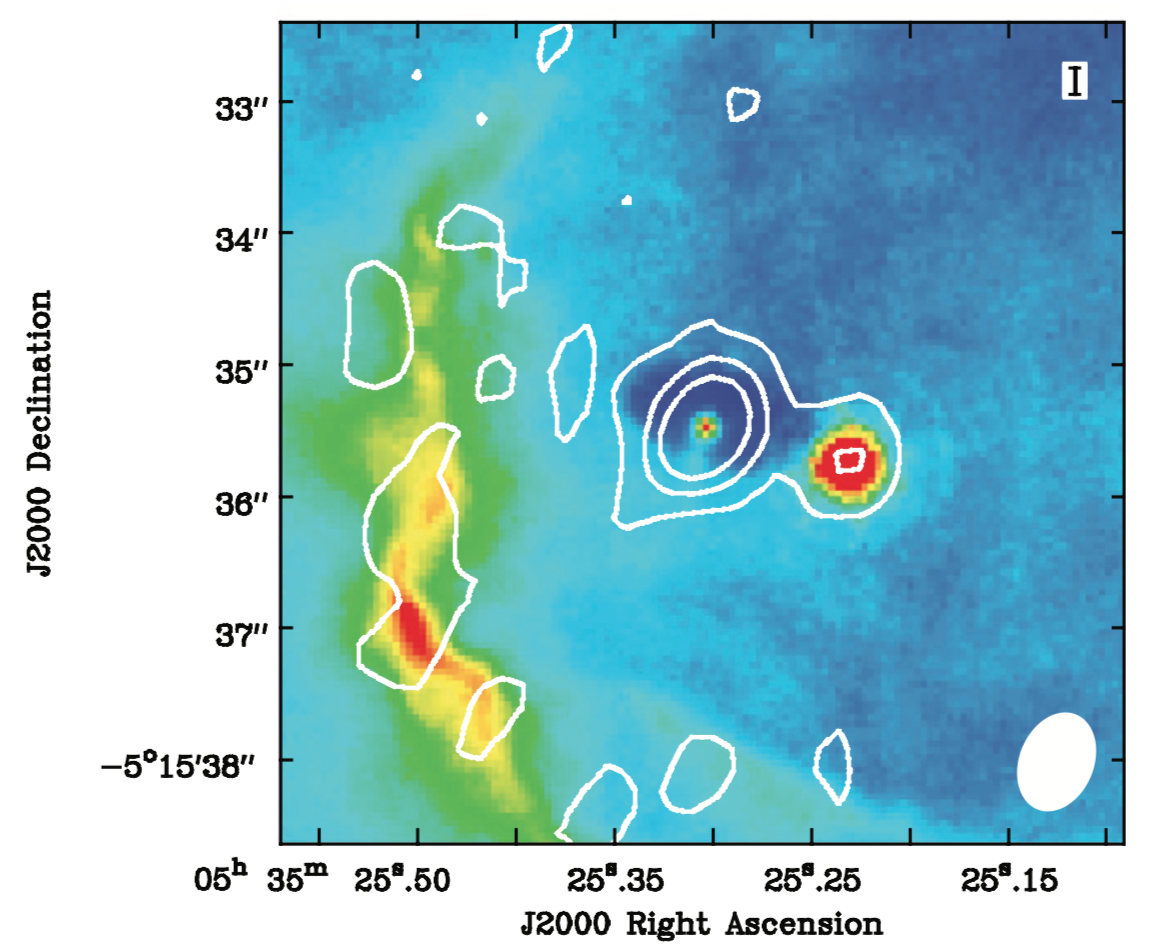
\includegraphics[width=0.33\linewidth]{V2434Ori_Ricci11.png}}\hfill%
  \hspace*{\fill}%
  \captionof{figure}{Images of V2434 Ori taken from \citet{Smith2005} on HST (Fig. \ref{fig:v2434ori_smith05}), \citet{MannWilliams2009} with the SMA at 880 $\mu$m (Fig. \ref{fig:v2434ori_mann09}), and \citet{Ricci2011} with the EVLA at 7mm (Fig. \ref{fig:v2434ori_ricci11}). The ionization front is clearly visible in both the HST and EVLA observations, and the jet from disk A is visible in the HST image.}
\end{figure}

First observed by \citet{Smith2005} using the Hubble Space Telescope, the authors took interest in what they saw as a binary system containing one star without a disk and one star embedded in a proplyd with a large jet and exhibiting tidal interactions with its companion (Fig \ref{fig:v2434ori_smith05}). \citet{MannWilliams2009} used 880 $\mu$m continuum measurements to estimate dust masses of the disks to be 0.066 M$_{\odot}$ and 0.018 M$_{\odot}$, for disks A and B respectively, making d253-1536a the most massive disk measured in the ONC, significantly larger than the Cluster's second largest disk at 0.034 M$_\odot$ and adding credence to the theory that $\theta^1$ Ori C is likely responsible for the truncation of disk masses in the Trapezium cluster. Subsequent detections at 7mm by \cite{Ricci2011} indicated that both disks are hosts to substantial populations of large dust grains (\ref{fig:v2434ori_ricci11}), although the distributions of grain sizes are different in the two disks. The same study also spectral typed the host of d253-1536b to be an 0.4 M$_\odot$ M2 star and a 3.5 M$_\odot$ G2 for d253-1536a's host star. This mass ratio of around 9:1 is somewhat atypically high for pre-main sequence binaries \citep{Duchene2013}.


\begin{figure}[htp]
  \hspace*{\fill}%
  \subcaptionbox{\label{fig:m1map_hco}}{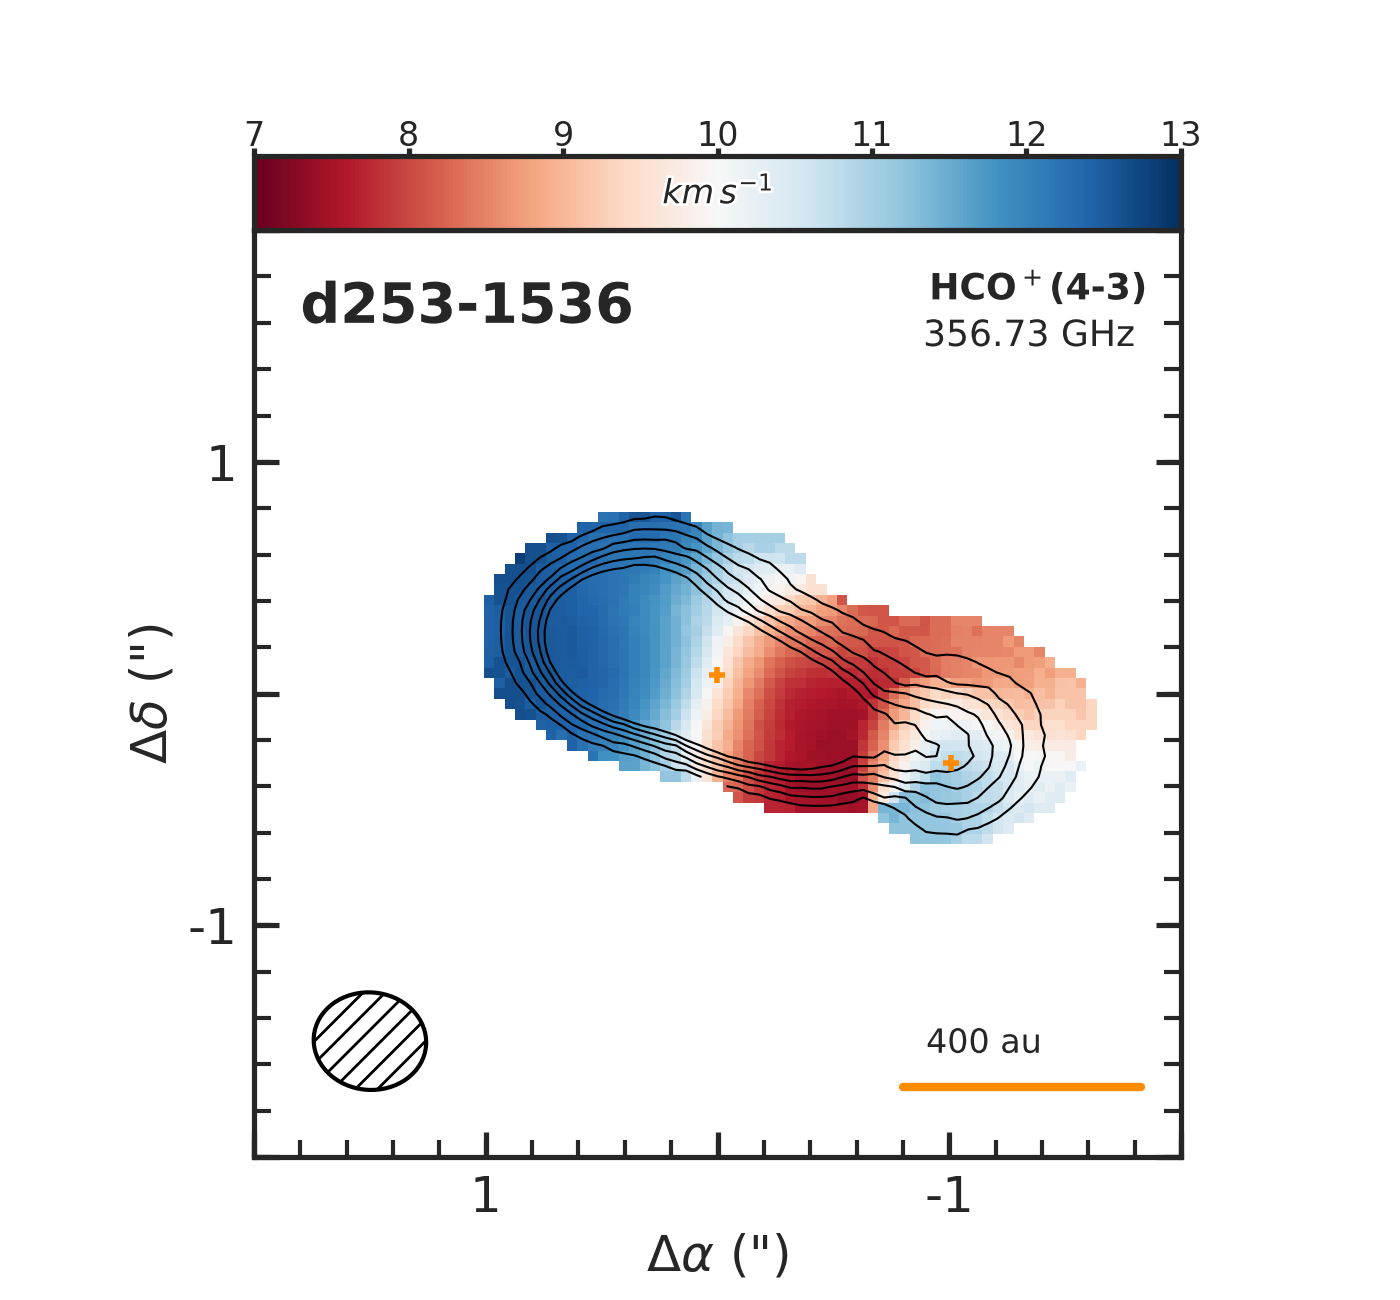
\includegraphics[width=0.25\linewidth]{moment1_hco-data.pdf}}\hfill%
  \subcaptionbox{\label{fig:m1map_hcn}}{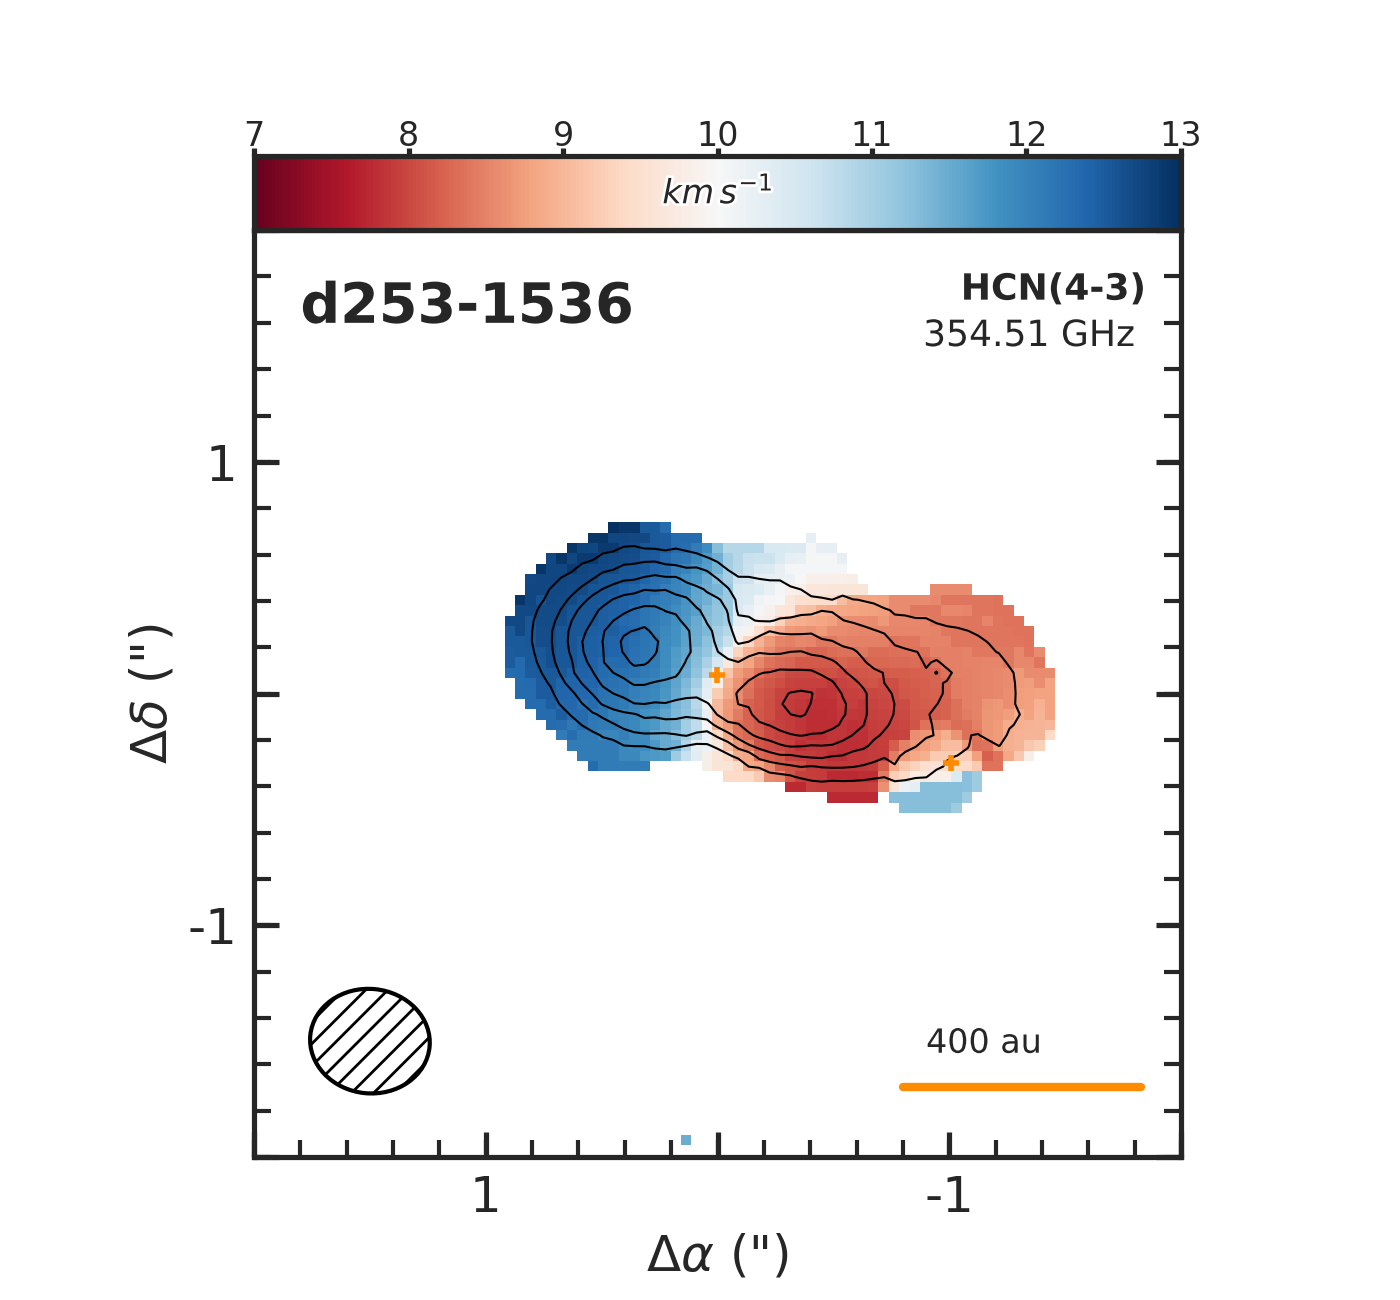
\includegraphics[width=0.25\linewidth]{moment1_hcn-data.pdf}}\hfill%
  \subcaptionbox{\label{fig:m1map_co}}{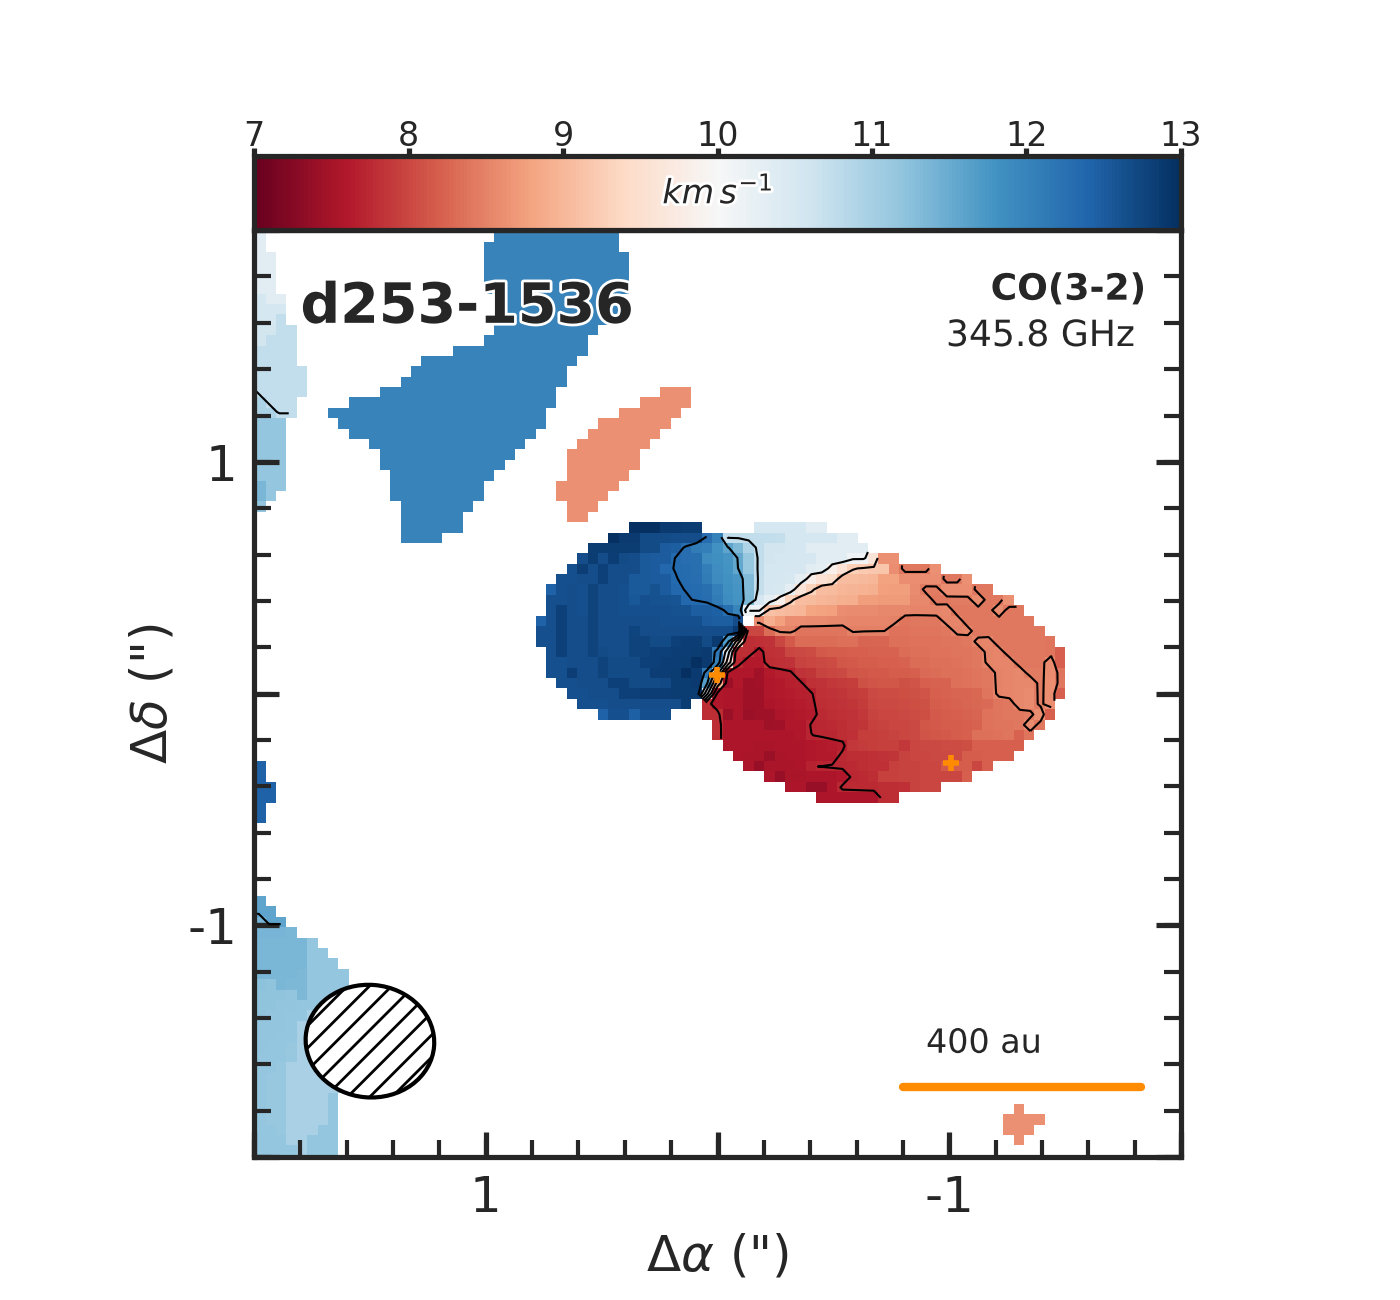
\includegraphics[width=0.25\linewidth]{moment1_co-data.pdf}}\hfill%
  \subcaptionbox{\label{fig:m1map_cs}}{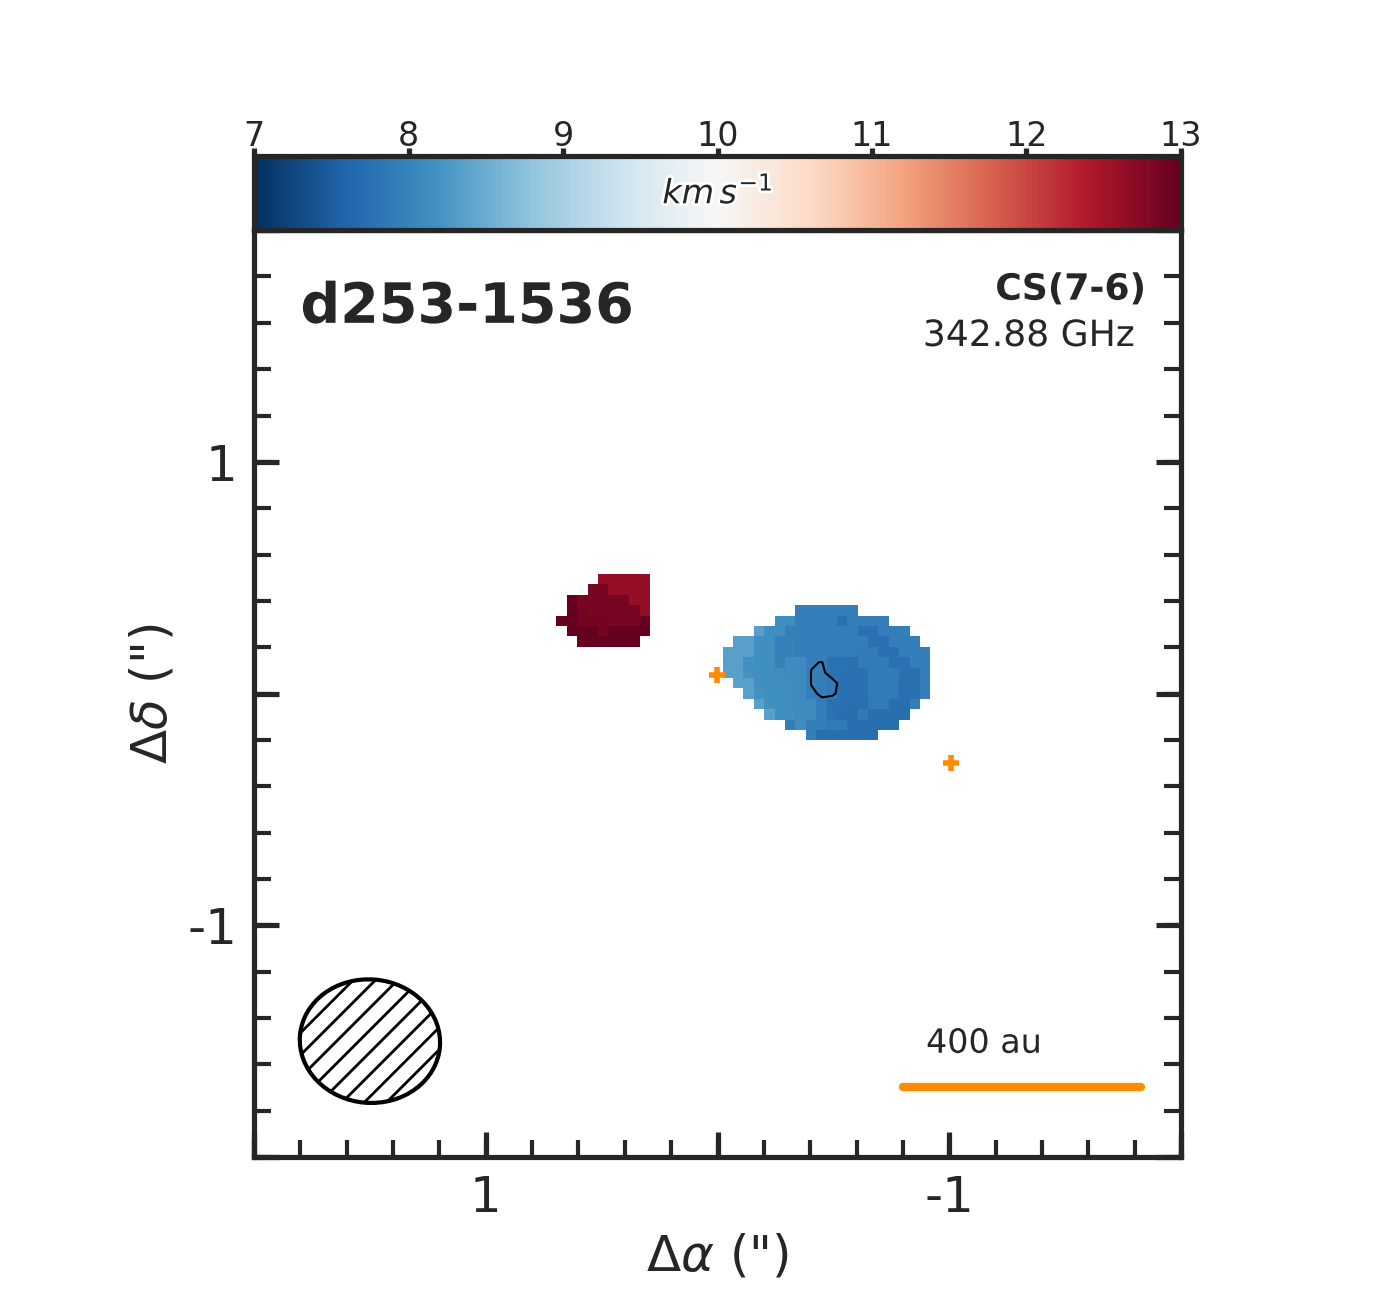
\includegraphics[width=0.25\linewidth]{moment1_cs-data.pdf}}\hfill%
  \hspace*{\fill}%
  \label{fig:m1map}
  \captionof{figure}{Moment-1 maps of HCO$^+$(4-3), HCN(4-3), CO(3-2), and CS(7-6) emission (left to right) in the present study's proplyds, observed with ALMA's Band 7. Each map shows intensity-weighted velocity, which allows us to trace the disks' kinematics. REWORK: considering making this a 2x2 grid, instead of 4 across.}
\end{figure}
% Need a more detailed figure caption.  What do all of the symbols on the map mean?  What object are we looking at?  With which telescope?  AT which frequency?  (Which transitions are these, specificaly?)  What do the contours mean?  What are the colors?  Take a look at some papers for examples of what information should go into a figure caption.


The system was observed in an ALMA survey of 22 proplyds in M43 by \citet{Mann2014} in four molecular lines (HCO$^+$(4-3), HCN(4-3), CO(3-2), and CS(7-6); Fig \ref{fig:m1map}), and preliminary fits of the system's kinematics in the HCO$^+$(4-3) line were made by \citet{Williams2014}. Using continuum observations alone and assuming canonical values for temperature, dust opacity, and gas-to-dust ratio, they found disk masses of 0.074 M$_{\odot}$ and 0.028 M$_{\odot}$ for disks A and B, respectively, larger than the previous values. They found an inclination for disk A of $i_A \sim 65^\circ$, but did not resolve disk B and thus were unable to determine its inclination. They found systemic LSRK velocities of 10.55 and 10.85 km/s for the two disks, which are close enough to be well within the escape velocity that the authors calculated for a disks at their projected separation of 440 AU of 2.5 km/s, indicating that the binary is bound. This similarity in systemic velocity also indicates that the binary's orbital plane is likely close to face-on.



With our high resolution observations of gas line emission, we aim to determine the temperature, density, and chemical profiles of the system, as well as refining the mass estimates for both disks and host stars. With this information in hand, we will examine this disk's characteristics in the context of previously studied disks in the Taurus and $\rho$ Ophiuchus star forming regions, as well as comparing it to the disk studied by \citet{Factor2017}, and evaluate the disks' planet forming potentials.






\section{Summary of Contents}

In this work we characterize ALMA observations of two young protoplanetary disks in the d256-1536 system. Observations and data reduction are described in \S2. In \S3, data and basic analysis are presented. Descriptions of modeling and fitting techniques are discussed in \S4, and in \S5, best-fit parameters are discussed and contextualized, as well as unexpected features maybe.
% Tossing a REWORK tag here so that I remember to get rid of that maybe.
% Also maybe combine the last paragraph of the previous section and Summary of Contents? They seem redundant.





















% The End

\chapter{Observations}
\label{chap:observations}

The data presented in this thesis are part of an ALMA survey of Orion proplyds in Orion (project 2011.0.00028.S); data collection and analysis methods of the continuum results are presented in \citet{mann_alma_2014}. Since this was part of a Cycle 0 Early Science project, the survey used only 22 of the array's 12 meter dishes in a hybrid configuration, with baselines ranging from 21.2 to 384.2 meters, yielding maximum angular scales and angular resolution of 8" and 0."5, respectively. At a distance of 389 pc, max angular scales and angular resolution correspond to 3,112 AU and 194 AU, respectively. The distance to the stars used here was recently measured by Gaia (\citet{gaia_collaboration_gaia_2016}, \citet{gaia_collaboration_gaia_2018}) to be 389 $\pm$ 7.97, nearer than the previous measurement of 414 pc.
% sig figs on the distance
% For Gaia references: https://gea.esac.esa.int/archive/documentation/GDR2/bib.html#bib173
\bigskip

Observations were made in Band 7 in four 1.875 GHz-wide bands arranged to cover the rest frequencies of the HCO+ (4-3), HCN (4-3), CO (3-2), and CS (7-6) transitions (356.734 GHz, 354.505 GHz, 345.796 GHz, and 342.883 GHz, respectively). Each band was split into 3840 channels with width 488.28 kHz, yielding a velocity resolution of 0.42 km s$^{-1}$.

\bigskip





Analysis showed that excluding baselines shorter than 110 k$\lambda$, 80 k$\lambda$, and 60 k$\lambda$ for HCO$^{+}$, HCN, and CO respectively optimized signal-to-noise ratios for each data set. The CS line showed no improvement with baseline cutting. This process is explained in greater detail in the Results chapter. \textit{more here? i.e. resolution or something}



These data, from Field 4 of \citet{mann_alma_2014} represent 13.6 minutes of on-source time. This duration was split into six 136 second observations, spaced out over 7.5 hours to ensure adequate \textit{uv} coverage. With the esulting in a synthesized beam of 0."57$\times$0."51 with a position angle of 85\degree. Precipitable water vapor in the atmosphere was stable at 0.7 mm.


The data were calibrated by ALMA staff using standard procedures in the Common Astronomy Software Applications (CASA, citation). The antenna-based complex gains and bandpass response of the system were calibrated using observations of the quasars J0607-085 and J0522-364 respectively. The absolute flux calibration was determined from observations of Callisto. The model of Callisto was drawn from Butler (2012) (citation). Absolute flux calibration is estimated to be accurate to within ∼ 10\% (\citet{mann_alma_2014}).

The velocity reference frame was converted from CASA's standard topocentric frame to LSRK (kinematic local standard of rest) using the CASA task \texttt{cvel}. Next, continuum emission was subtracted in the uv plane using the CASA task \texttt{contsub}. Visibilities were then inverted with natural weighting, deconvolved, and restored using standard procedures from the Multichannel Image Reconstruction Image Analysis and Display, or MIRIAD, package (\citet{rj_sault_astronomical_1995})








\iffalse
Things to get:
* Does ICR use natural weighting? (using robust=2)
\fi
% Note that no closing info is needed.

\chapter{Results}
\label{chap:results}

\section{Modeling}
% Ex footnote: \texttt{K2Phot}\footnote{\href{https://github.com/vincentvaneylen/k2photometry}{https://github.com/vincentvaneylen/k2photometry}} \citep{vaneylen2016}


Spatially and spectrally resolved line emission was detected for CO (3-2), HCO$^{+}$ (4-3), HCN (4-3), and CS (7-6) across around 50 channels of width 0.42 km s$^{-1}$. Detailed studies of gas structure in protoplanetary disks are still relatively rare, and have previously only fucsed on disks in nearby low-mass star-forming regions (SFRs). Consequently, it would be useful to develop a rough understanding of the observations before beginning detailed modeling. This includes removing cloud contamination, investigating the general morphology of the disks using moment maps, estimating the disks' gas masses using integrated line flux, and examining the velocity profile to estimate the mass of the central star (really?).

Cloud contamination occurs when emission from background or foreground gas clouds is detected in the same direction as the disk being observed. Since the Orion Nebula has a higher gas density than in low-mass SFRs, cloud contamination is more much common and problematic. "Previous observations of these disks by Mann & Williams (2009) (citation) (do I have these?) strongly detected the CO (3-2 line)". Thanks to the higher sensitivity of the ALMA observations, etc.

CO displayed the most significant cloud contamination, thanks to its low critical density and higher abundance in the clouds. For the other molecular lines, which have higher critical densities, cloud contamination is less severe but still clearly present in HCO$^{+}$, which is the brightest tracer.

Since cloud contamination inherently tends to be large-scale in structure, excluding short baselines reduces its contribution to the observations. While this process slightly reduces the total recovered flux from the disk and our ability to characterize its large-scale strucutre, it is necessary to avoid including cloud emission from the cloud in the process of fitting the disk emission. By evaluating mean and RMS noise for an off-source region of the field while varying the minimum baseline used, we found that excluding baselines less than 110 k$\lambda$, 80 k$\lambda$, and 60  k$\lambda$ for HCO$^{+}$, HCN, and CO, respectively, yielded optimum results. Since the CS line already has a very low SNR and a higher critical density, excluding baselines did not improve the observations.





Table 1: Integrated Flux Measurements
Line       | Baselines                   | Max Angular Scale | Integrated Line Flux (Jy km s$^{-1}$)
CS (7-6)    All
CO (3-2)    All
CO (3-2)    \textgreater 60 k$\lambda$
HCN (4-3)   All
HCN (4-3)   \textgreater 80 k$\lambda$
HCO$^{+}$   All
HCO$^{+}$   \textgreater 110 k$\lambda$


Figure 1:

\begin{figure}
  \centering
  \includegraphics[height=0.8\textheight]{Noise-copmarison-HCO+_mom0.pdf}
  \caption{blah}
\end{figure}

The effects of these exclusions are detailed in Table 1 and demonstrated on the HCO$^{+}$ line in Figure 1. (Analysis of these plots, bottom of p.3 in Factor et al)


In all lines, rotation of each disk is clearly visible as a transition from red-shifted emission in one corner to blue-shifted emission in the other corner***. The maximum extent of the 3-$\sigma$ contours along the disks' major axes correspond to outer diameters of the HCO+ disks of A and B; outer diameters of the HCN disks of A and B; and outer diameters of the CO disks of A and B, all at a distance of 389pc. The CS emission is not detected strongly enough to provide a reliable measurement (check that this is true)

Tables 2 and 3 present the velocity-integrated line fluxes and the best-fit parameters for a simple elliptical Gaussian fit to the visibilities for each disk, respectively. Integrated line flux was measured using the MIRIAD task cgcurs to integrate the intensity in the zeroth-moment map throughout the region enclosed by the 3 $\sigma$ contour level. Uncertainties in the integrated line flux do not include the 10\% absolute flux calibration uncertainty inherent in the ALMA observations caused by uncertainties int he models of solar system objects used as flux callibrators. Elliptical Gaussian fits of the visibilities were performed using the MIRIAD task uvfit.

Assuming optically thin emission (maybe good?) and Local Thermodynamic Equilibrium (LTE), the line-emitting gas mass, M$_{\text{gas}}$ is given by:

\begin{align}
  M_{\text{gas}}= \frac{4 \pi}{h \nu_0} \frac{F m d^2}{A_{ul} X_u},
\end{align}

where $F$ is the integrated line flux, $m$ is the mass of the emitting gas molecule, $d$ is the distance to the source, $h$ is the Planck constant, $\nu_0$ is the molecular line's rest frequency, $A_{ul}$ is the Einstein coefficient for the ($u - l$) transition, and

\begin{align}
  X_u = \frac{N_u}{N_{\text{tot}}} = (2 J_u + 1) \frac{\exp [-B_0 J_u (J_u + 1) h c/kT_{\text{ex}}]}{kT_{\text{ex}}/hc B_0}.
\end{align}

In (2), $\frac{N_u}{N_{\text{tot}}}$ is the ratio of the number of molecules in the upper state to the total number of molecules; $J_u$ is the quantum number of the upper level; $B_0$ is the rotation constant in units of wavenumber; $h$ and $c$ are the Planck constant and speed of light, respectively; and $T_{\text{ex}}$ is the excitation temperature. VALUES FOR A_UL AND B0 WERE TAKEN FROM MOLECULAR DATA MADE AVAILABLE BY SHOIER ET AL 2005. LOTS MORE TO DO HERE.


A position-velocity diagram for HCO$^{+}$ is shown in Figure 4, showing the position, as a function of velocity, of emission form a cut along the major axis of the disk (FIGURE OUT HOW TO DO THIS).
ANALYSIS of this stuff.




To find best fit values, we use disk modeling and ray-tracing code developed by \citet{flaherty2013}. The code turns a set of paramters describing the disk's physical structure (atmospheric temperature, density structure, molecular abundances, and so on) into a three dimensional model. Given observational characteristics (distance, inclination, and so on), it can then turn that model into a simulated sky-projected image which may then be compared to our observational data.

Explorations of paramter space were implemented through



Things to get:
* Rewrite this whole thing.
* Previous observation of these disks with SMA? Maybe Mann & Williams 2009. What did they detect?
* Integrated Flux Measurements
* Make a 2-image subplot of HCO+ with and without baseline cutting. Moment 0 or Moment 1? Show n-sigma contours
  * Find max width of disks for each line by 3-sigma contour

* Make moment0 and moment1 plotters. Two panel or just 1? Should have contouring.
* Use cgcurs to get integrated line flux in moment0 map.
* use uvfit for elliptical guassian vis fits.
* PV Diagram
* Gas mass calculations





% Note that no closing info is needed.

\chapter{Analysis}
\label{chap:analysis}

By modeling spatially and spectrally resolved obserations of protoplanetary disks, we can measure their chemical and physical characteristics. To model the system, we generate a synthetic image of what a disk with known physical characteristics (like disk radius, mass, and so on) would look like at a certain distance, inclination, and position angle relative to us. From that synthetic image, we may generate a synthetic set of visibilities, and then compare those visibilities to our observations. By iterating this process, we may generate many models with different parameter combinations and evaluate how well each resulting model disk matches our observations. We use a Markov Chain Monte Carlo technique described in \S\ref{subsection:mcmc} to explore the parameter space and measure the physical properties of the disk.

% It’s not just the aggregation, but rather the iterative process itself that allows us to explore parameter space.  Also, MCMC doesn’t just tell us the best fit values, but, critically, how well we know those values (the uncertainties that we get from the PDF).

In \S\ref{section:gas_model}, we describe the basic equations and computational processes that generate the model disks. In \S\ref{section:param_space}, we describe how, once models are made, we may move through high-dimensional parameter space to identify regions of best-fit. Finally, in \S\ref{section:fitting_procedure}, we present the results of our fitting procedures.


\section{Gas Model}
\label{section:gas_model}

In this work, we use a gas-disk model originally developed by \citep{Rosenfeld2012,Rosenfeld2013} and translated from IDL to Python by \cite{Flaherty2015}. The code assumes that Local Thermal Equilibrium\footnote{This may or may not be a valid assumption in protoplanetary disks, but \cite{Pavlyuchenkov2007} showed that it was appropriate for CO.} (LTE), and hydrostatic equilibrium. The code draws on user-input temperature- and surface-density profiles to calculate a vertical density structure, and calculates the velocity field based on the stellar mass. It then performs radiative transfer on the resulting structure to create a sky-projected image of the model disk, taking into account line thermal and turbulent line broadening. By assuming LTE and hydrostatic equibilibrium, the code is able to to run quickly enough to allow for a Markov Chain Monte Carlo routine to generate models on a reasonable timescale, as described in \S\ref{subsection:mcmc}




\subsection{Establishing Physical Profiles}
A circumstellar disk can be characterized by three major profiles: its radial and vertical temperature structures, its radial and vertical density structures, and its velocity field. Generating a model disk is a matter of defining these three functions.


% However, these are complex functions, and the reality that they attempt approximate is not necessarily a well-behaved, simple one; no disk's density actually falls off exponentially, although in some cases it can be well approximated as such (\cite{Hughes2008}, \cite{Williams2011}). Furthermore, even these approximations often cannot be solved analytically, instead relying on numerical integration to be solved, which is a computationally expensive task. Therefore, we choose to make certain simplifying assumptions which, although they come at a cost to realism, enable significantly increased computation speeds.

% Are you specifically talking about the hydrostatic equilibrium condition here?  If so, say it!  I can’t think of anything else that requires numerical integration to solve in the code… unless you’re talking about some sort of arbitrary functional form, but that would not be motivated by theory, and not really by observations either.  There are a lot of good reasons why we assume these functional forms, not just because they’re fast!

% LTE is the only assumption that really increases the computation speed — so if that’s what this paragraph is about you should say it explicitly.  Right now you’re conflating the functional forms of the density/temperature/velocity profiles with the physical assumptions of LTE and hydrostatic equilibrium, so please try to separate those out.  (There is excellent evidence that these disks are well described by a Keplerian velocity profile in hydrostatic equilibrium — that’s basically what Katherine Rosenfeld’s 2013 paper on HD 163296 was about!).  

% Wait, what?  That’s not what LTE means.  Also, you have a 2-D temperature profile, not a 1-D temperature profile!  Do a little more reading about LTE and try again. :-) REWORK


For the disk's temperature profile, we draw on the parametrization of disk temperature structure first laid out by \cite{Dartois2003}, where the disk's temperature is given by,

\begin{align}
  T_{\text{gas}}(r, z) = \begin{cases}
                          T_a + (T_m - T_a) \left[ \cos \frac{\pi z}{2 z_q} \right]^{2\delta} \text{   if } z > z_q \\
                          T_a \text{   if } z \leq z_q(r).
                         \end{cases}
\end{align}

The atmospheric temperature and mid-plane temperatures are given by $T_a = T_{atm,150} (r/150 \text{AU})^{q}$ and $T_m = T_{mid, 150} (r/150 AU)^{q}$, where $q$ is typically negative and controls the functions' decay. Since $T_m$ is smaller than $T_a$, the second term of the low-scale height temperature function is negative, so the sinusoid effectively implements a decreasingly-negative contribution to the temperature with hight above midplane.  The disk's scale height, controlled by $z_q$ is assumed to be radially increasing, as described by a power law, $z_q(r) = z_{q,150}(r/150 \text{AU})^{1.3}$. $\delta$, a tunable exponent controlling the rate of the disk's vertical temperature decay, is set to 1, though it can take on values between 1-2 (\cite{Dartois2003}).


The disk's velocity field is assumed to be Keplerian with slight corrections for gas pressure support and the addition of a vertical dependence. The assumption of Keplerian veloicites is generally valid in the case that $M_{\text{disk}} \ll M_{\star}$, which continuum observations of the system have shown to be the case for the disks in this system (readers interested in a deeper explanation of the velocity field derivation are referred to \cite{Rosenfeld2013}). With these corrections added, the model disk's velocity field is given by


\begin{align}
  \frac{v_\phi^2}{r} = \frac{GM_\star r}{(r + z)^{3/2}} + \frac{1}{\rho_\text{gas}} \frac{\partial P_\text{gas}}{\partial r};\,\, v_r = v_z = 0.
\end{align}


The final structure we would like to define is the gas density profile. By assuming hydrostatic equilibrium, we may relate the disk's gas density and temperature profiles as

\begin{align}
  -\frac{\partial \ln \rho_\text{gas}}{\partial z} = \frac{\partial \ln T_\text{gas}}{\partial z} + \frac{1}{c_s^2} \left[\frac{G M_{\*} z}{(r^2 + z^2)^{3/2}} \right].
\end{align}

Here $c_s$ is the local sound speed, given by $c_s^2 = \frac{k_B T_\text{gas}}{\mu m_H}$, $T_\text{gas}$ is the temperature profile given above, $m_H$ the mass of hydrogen, and $\mu$ is the mean molecular weight of the gas, set here at 2.37 to reflect the gas's 80\% H$_2$ composition. We may solve this equation by integration, giving us the disk's density profile $\rho(r, z)$.


The model's surface density profile is drawn from \cite{Hartmann1998}, in which they expanded on the work of \cite{LyndenBell1974} to show that the structure of an isolated disk with viscosity given by $\nu \propto R^\gamma$ is well-described by


% Also, isn't this Hughes2008's equation?

\begin{align}
  \Sigma_{\text{gas}}(r) = \frac{M_{\text{gas}} (2 - \gamma)}{2 \pi R_c^2} \left(\frac{r}{R_c} \right)^{-\gamma} \exp \left[-\left(\frac{r}{R_c} \right)^{2-\gamma} \right],
\end{align}


where $R_c$ is the radial extent of the gas disk, $\gamma$ is a power law index, and $M_\text{gas}$ is the total gas mass. This form allows the disk to behave as a power law radially until R$_c$, at which point it turns over into exponential decay. \cite{Hughes2008} showed that exponentially tapering the disk's outer radius, rather than sharply cutting it, provides the best agreement between gas and disk outer radii. We may safely approximate $M_\text{gas} = M_\text{disk}$, since at this early stage in the disk's development, the gas is by far the majority element of the disk's mass total.

% REWORK (on temp freezeout dropoff): Hm, this reminds me that Charlie Qi recently showed that freeze-out is less abrupt than this, so we should probably do something a bit more gradual for freeze-out (I thought Kevin had implemented this, but maybe not in the version of the code that you’re using).  It’s not extremely high-priority, but you should check out Charlie’s (Chunhua’s) papers and make sure you know what I”m talking about and then think about how we could do this better.  


Modifications are made to this density profile in two cases. At sufficiently low temperatures, molecules will condense out of the gas phase. The mid-plane of the disk is sufficiently cold to prompt this behavior. We may simulate this behavior by dropping the gas density by a factor of $10^{-18}$ wherever the temperature falls below some characteristic freeze-out temperature, T$_{FO}$, a temperature which is molecule-specific. Conversely, at the disk's upper surface, photodissociation by stellar and interstellar radiation dominates, so we implement a decrease in density wherever the hydrogen column density at the disk's surface falls below a characteristic value. We use values drawn from \cite{Factor2017} for these parameters, presented in Table \ref{tab:mol_specifics}. The resulting temperature and density structure of a typical proplyd is shown in Fig \ref{fig:temp_dens_str}.


\begin{table}
  \begin{threeparttable}
    \centering
    \caption{Molecule-specific values}
    \label{tab:mol_specifics}
    \renewcommand{\arraystretch}{1.2}
    \begin{tabular}{c  l  c c }
      \toprule \toprule
      \multirow{2}{*}{Parameter} & \multirow{2}{*}{Description}    & \multicolumn{2}{c}{Fixed Value(s)} \\
                                 &                                 & CO, HCO$^+$ & HCN \\
      \midrule %\midrule
      T$_{FO}$            &  Molecular freeze-out temperature      &  19 & 60    \\
      $\sigma_\text{Max}$ & Column density upper limit &  [$1.3 \times 10^{30}] \text{cm}^{-2}$ & $9.5 \times 10^{21} \text{cm}^{-2}$  \\
      \bottomrule
    \end{tabular}
    \begin{tablenotes}\footnotesize
      \item[*] Values drawn from \cite{Factor2017}
    \end{tablenotes}
  \end{threeparttable}
\end{table}



\begin{figure}[htp]
\centering
  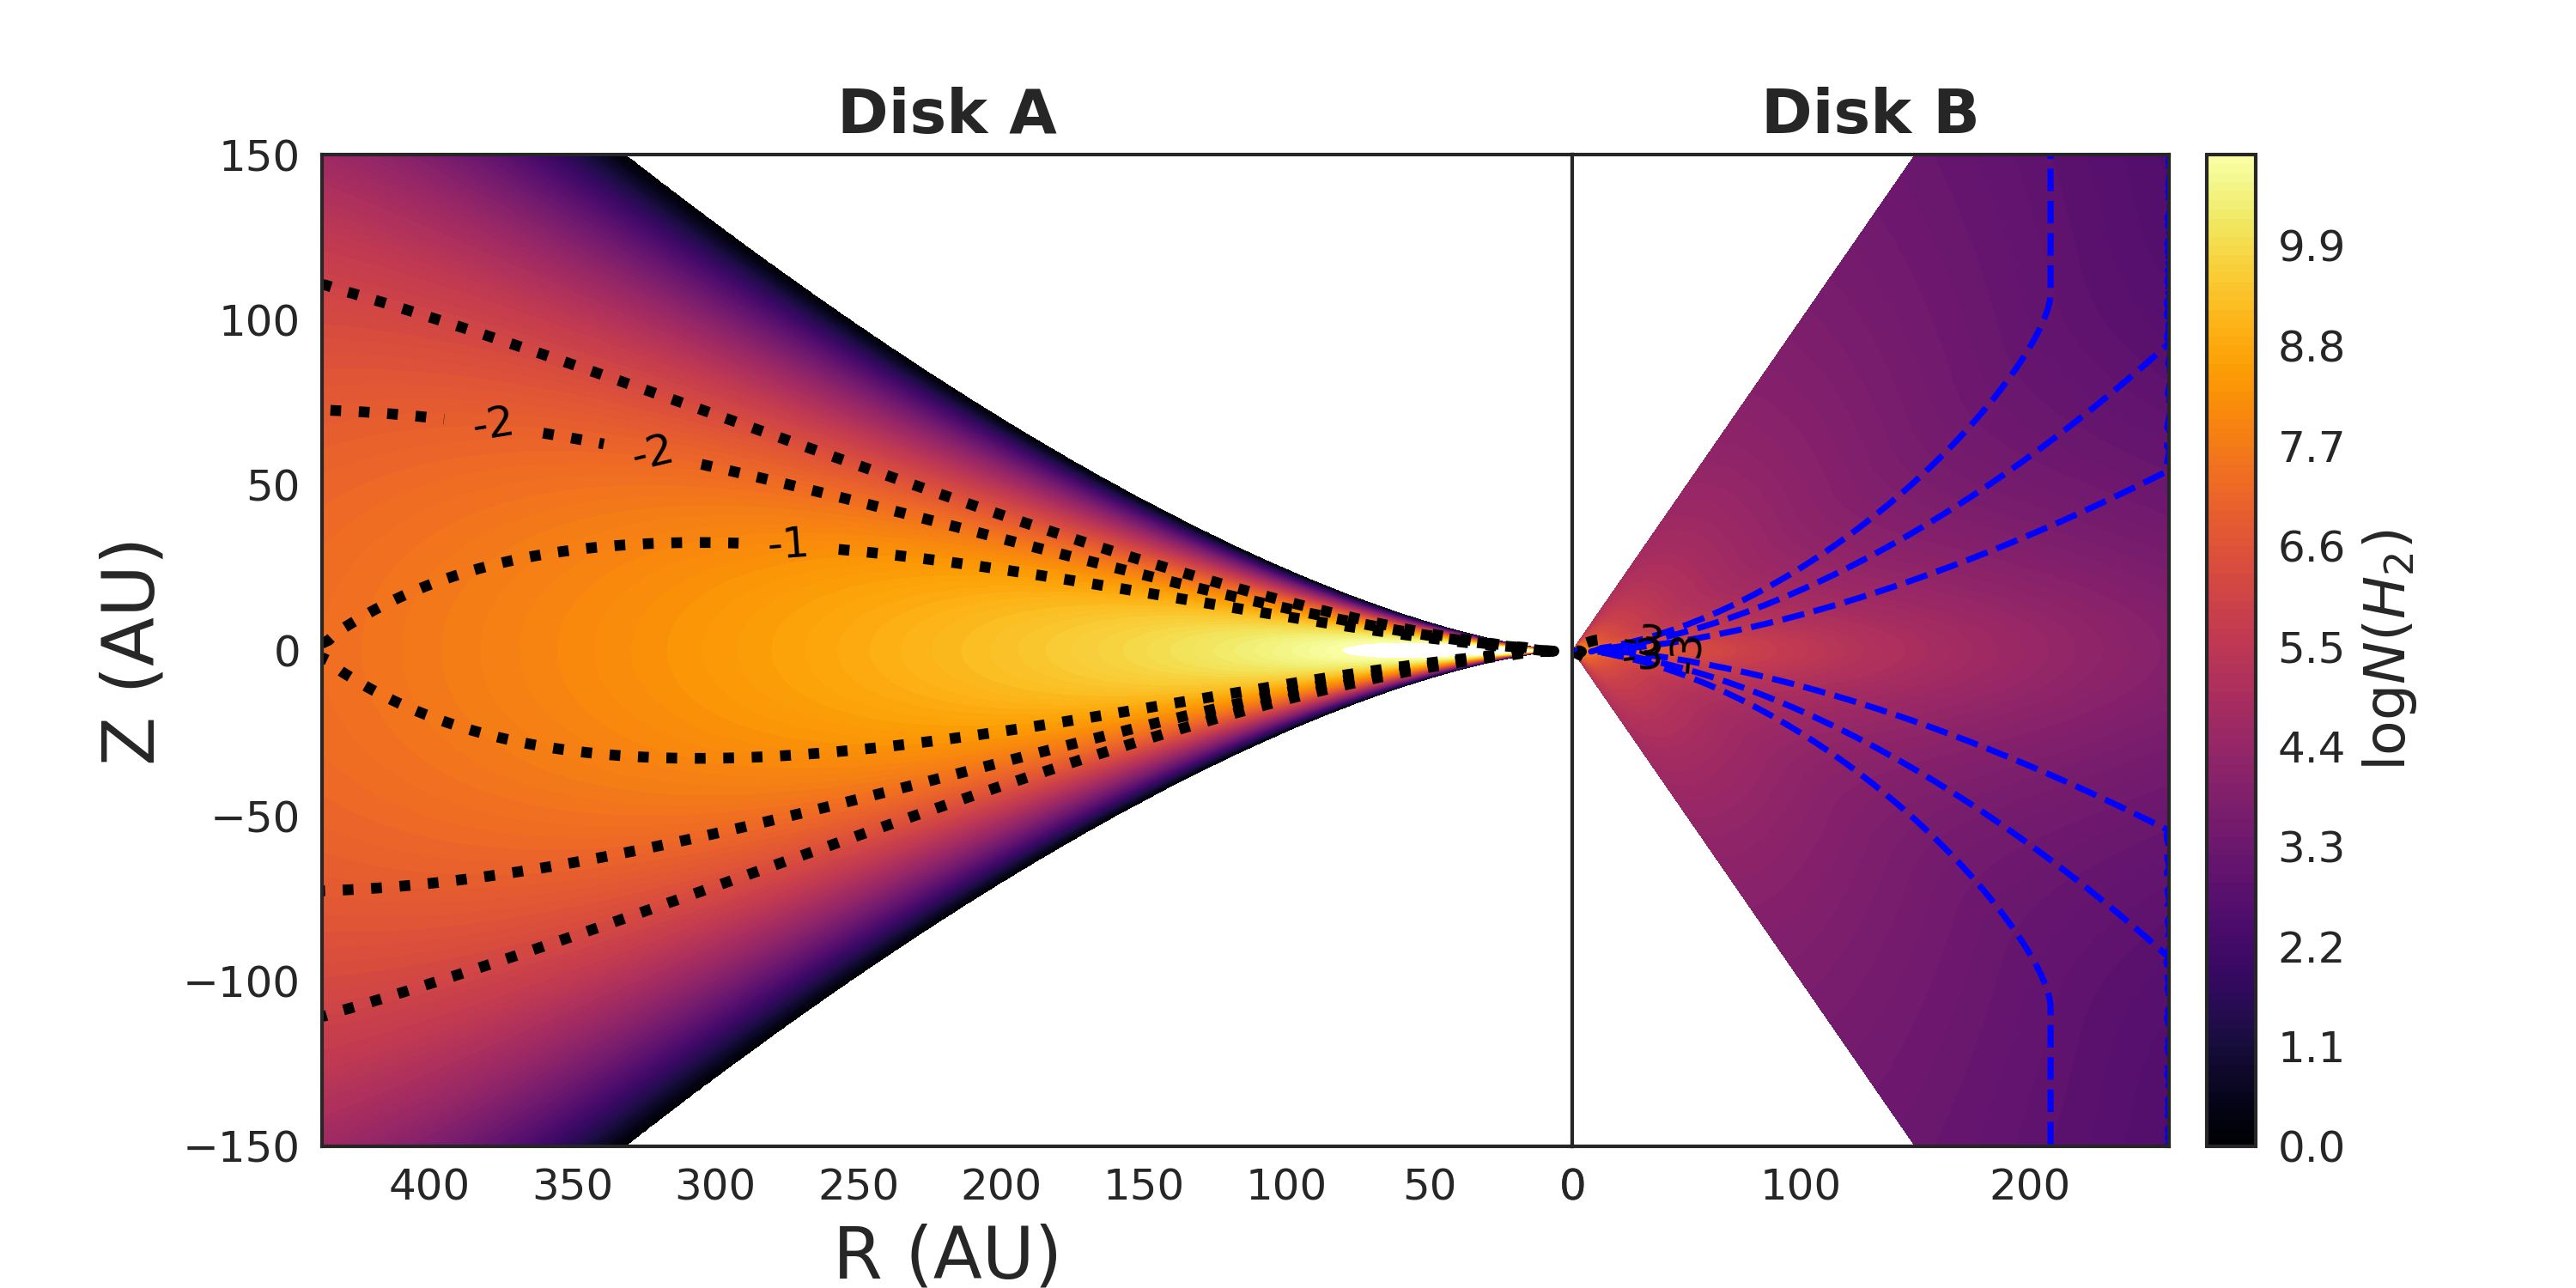
\includegraphics[width=\linewidth]{example-disk-strs.png}
  \captionof{figure}{Radial and vertical temperature structures for disk A \textit{(left)} and disk B \textit{(right)} in CO. We may quickly see that disk A has a larger radial extent and a better defined profile, thanks to its higher signal.}
  \label{fig:temp_dens_str}
\end{figure}
% REWORK: Need a much more informative caption!  Check Sam’s paper for examples if you need them. Also, make the labels bigger on the color bar to the right for readability.  Add units to the label too (both on the color bar and on the contours in the figure).
% I guess go into Kevin's code and chop up? Or just copy/paste it out into analysis or something.





\subsection{Generating a Model Image}

Having now established our model disk's physical structure through temperature, density, and velocity profiles, we may begin generating an image of the disk by calculating flux contributions through the disk. To do so, we calculate the specific intensity by integrating the equation of radiative transfer:

\begin{align}
  I_\nu = \int_0^{\infty} K_\nu(s)\ S_\nu(s)\ e^{-\tau_\nu(s)}\ ds,
\end{align}

where $K_\nu(s)$ is the absorption coefficient, $\tau_\nu(s)$ is the optical depth and is defined as $\tau_\nu(s) = \int_0^s K_\nu(s') ds'$, and $S_\nu(s)$ is the source function. Since disks emit as blackbodies, the Planck function, $B_\nu(T)$, is used as the source function. Line broadening, a function of temperature and disk turbulence, is added, and the resulting flux is Doppler shifted to account for the disk's specified systemic velocity. Finally, the image is scaled, shifted, and rotated to account for the source's distance ($d$), angular offset from the center of the image ($\Delta \alpha$ and $\Delta \delta$), and position angle and inclination (PA and $i$) relative to our viewing direction.
% REWORK: Add an explanation of how I got positional offsets
% REWORK: Baseline cutoff explanation. Does that happen in a different chapter? Maybe should happen here.

Since the model disk is fully defined at every point in both physical and velocity space, we may set the spatial and spectral resolution to ensure that it is sampled well compared to the resolution of the data. We set our spectral resolution to match that of our observation, while we let the spatial resolution be $\sim$ 1/10 the size of the synthesized beam. This resolution is high enough to avoid sampling artifacts when we simulate interferometric observations of the image.

% REWORK: Random thought as I’m reading this: can you please check whether or not Hanning smoothing is implemented in the MIRIAD commands that Kevin’s code uses?  Before uvmodel, there should be a “hanning” command in MIRIAD… let me know.  (If not, we should add it.)

We then use the Miriad task \texttt{uvmodel} to generate visibilities from the model image, sampled in the same $uv$ tracks as our observation. The $\chi^2$ statistic is then used as a goodness-of-fit metric to compare the data and model in the visibility domain. We make this calculation in the visibility domain, rather than the image domain, so that the resulting $\chi^2$ value is not influenced by artifacts generated in the imaging process.


We now have the ability to generate a model disk, first by calculating its physical structures (in radial temperatures, densities, and velocities), then by drawing on radiative transfer to calculate the flux contributions from the disk. That flux is sky-projected to match the observed source's orientation, and the resulting image is then transformed from the image domain to the visibility domain and its fit quality evaluated.



\section{Exploring Parameter Space}
\label{section:param_space}

Now that we have the tools available to generate synthetic images that are tuneable across a large number of parameters, we must decide how best to move through that large parameter space to find a best-fit region. To do so, we use two methods.

\subsection{Grid Search}
\label{subsection:grid_search}
The first, and perhaps most intuitive, way to move through this parameter space is using a simple grid search. A grid search involves manually assembling lists of values to try for each parameter and then generating models and calculating the resulting $\chi^2$ value for every possible combination of parameters in those lists. A best-fit value is recovered by simply finding the point in that $n$-dimensional grid that yielded the best $\chi^2$, and then either calling that position in parameter space a best-fit location or then defining a finer grid around that point and repeating the process until an acceptable resolution has been reached. Benefits of grid search include its relatively straightforward nature (the the consequent simplicity of implementation) and its usefullness as a diagnostic tool, since very specific regions of parameter space may be sampled with the manual entry of positions to test. However, it is a relatively simple method and leaves room for improvement.

Grid search was used to locate the disks in $(\alpha, \dec, v)$ space. All other parameters were fixed at best-guessed values, then grids were run with resolutions sufficiently fine to meet the observations' spatial and spectral resolution. Grids for the disks' systemic velocities were centered at values found in \cite{Williams2014}, while $\Delta \alpha$ and $\Delta \dec$ offsets were first approximated using the MIRIAD task \texttt{uvfit} to fit a Gaussian to each disk. The resulting centroids were used to center the grids for refinement.


\subsection{Markov Chain Monte Carlo}
\label{subsection:mcmc}

Markov Chain Monte Carlo (MCMC) algorithms offer us a way to both sample the probability distribution of a complex parameter space (much like a grid search), but offer an improvement over grid search by yielding the posterior probability distribution of each point, allowing us to characterize the uncertainty associated with each best-fit value with error bars. We use an affine-invariant formulation of the MCMC algorithm described by \cite{Goodman2010} and implemented in the Python package \textittt{emcee} by \cite{ForemanMackey2013}.

MCMC routines sample the probability distribution of a given $n$-dimensional parameter space by deploying an army of "walkers." Each walker begins at some initial position, evaluates the $\chi^2$ value of that point, and then proposes moving to a new position in parameter space according to a Gaussian probability distribution centered at the current point and decaying with distance (so that nearer points are preferentially - but not necessarily - selected). The $\chi^2$ value of this new position - or "step" - is then evaluated, and is either accepted (the walker moves to that position) or rejected (the walker remains where it is and repeats the new-step proposal process) with probability $p = \exp \left[ (\chi_\text{current}^2 - \chi_\text{new}^2)/2 \right]$ (is this only for Metropolis Hastings?). This function indicates that if the proposed step yields a better fit (a lower $\chi^2$ value) than the current position, $p > 1$ and the step is accepted. However, if proposed step results in a worse fit, there is still a non-zero chance that the step is accepted, proportional to how much worse it is. This willingness to accept an increased $\chi^2$ value allows the walker to avoid becoming trapped in local minima. The list of steps taken by each walker and their accompanying $\chi^2$ values are compiled into the "chain" part of Markov Chain Monte Carlo. \cite{Goodman2010} show that a walker's desire to remain in a location is proportional to the local probability density, meaning that we may infer uncertainties in our fits from the density of walker steps taken in a region.

We may introduce boundaries to the parameter space explored by our walkers using "priors." These priors are manually set, and allow us to restrict the walkers' motions into regions that we know a priori to be implausible fits. Justifications for these constraints are either mathematical (e.g. disk should not have a negative radius) or physical (e.g. both disks' radii are clearly far less than 1000 AU). These priors may be either uniform, with hard cuts at their bounds, or Gaussian, with preferential treatment given to walkers closer to the Gaussian centroid (a known value).

We may visualize the results of the walkers' journeys using corner plots. Corner plots allow high-dimensional space to be visualized in two dimensions by taking slices across each pair of axes and showing the density of samples drawn in that slice. In each of these slices, a perfectly certain fit would appear as a very tight, point-like Gaussian - the sample density around the best fit would be extremely high and low everywhere else, as the walkers quickly converged and remained on that best fit point - while conversely, higher uncertainties are shown by a wide spread of samples around the central point. Degeneracies between parameters can be seen as streaks in these corner plots, showing a correlation. Corner plots for Disk A and B in an HCO$^+$ fit are shown in Figs \ref{fig:corner_a} and \ref{fig:corner_b}, respectively.


\begin{figure}[htp]
  % Maximum length
  % \subcaptionbox{1a\label{fig1:a}}{\includegraphics[width=1.6in]{example-image-a}}\hfill%
  % \subcaptionbox{1b\label{fig1:b}}{\includegraphics[width=1.6in]{example-image-a}}%
  % \bigskip
  % Equal length
  \hspace*{\fill}%
  \subcaptionbox{Disk A fits \label{fig:corner_a}}{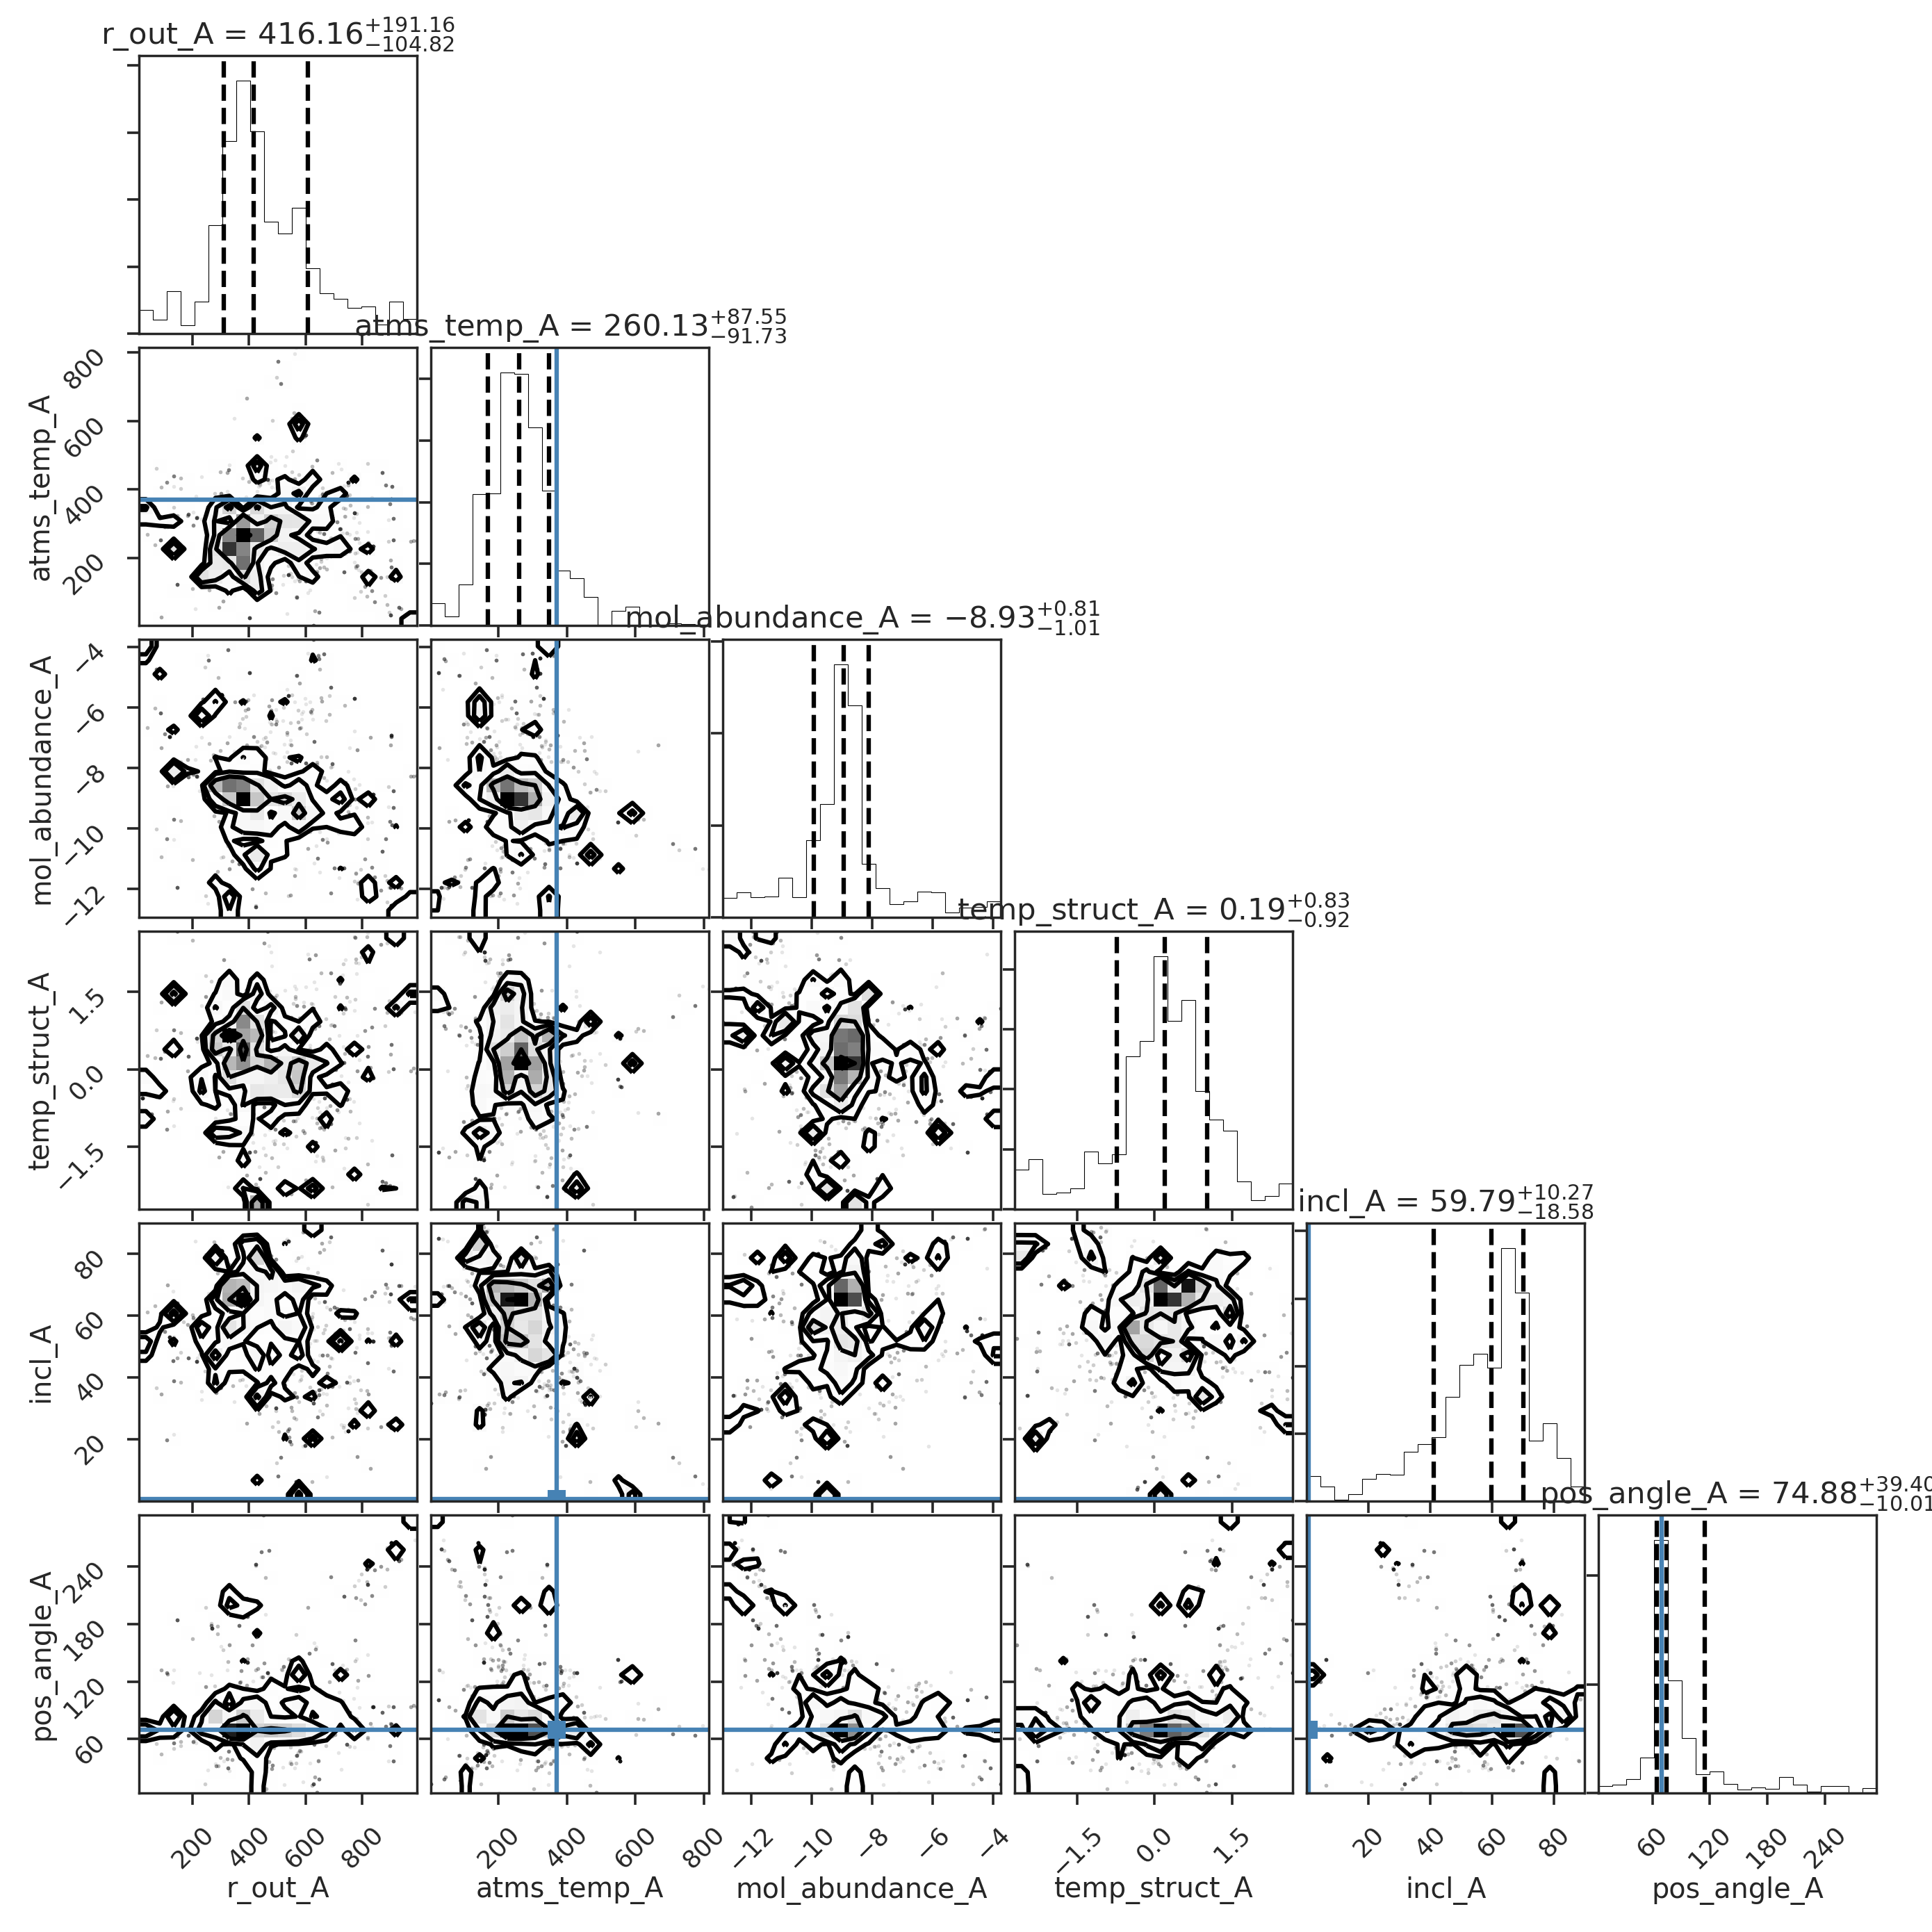
\includegraphics[width=0.49\linewidth]{cornerplot-diskA.png}}\hfill%
  \subcaptionbox{Disk B fits \label{fig:corner_b}}{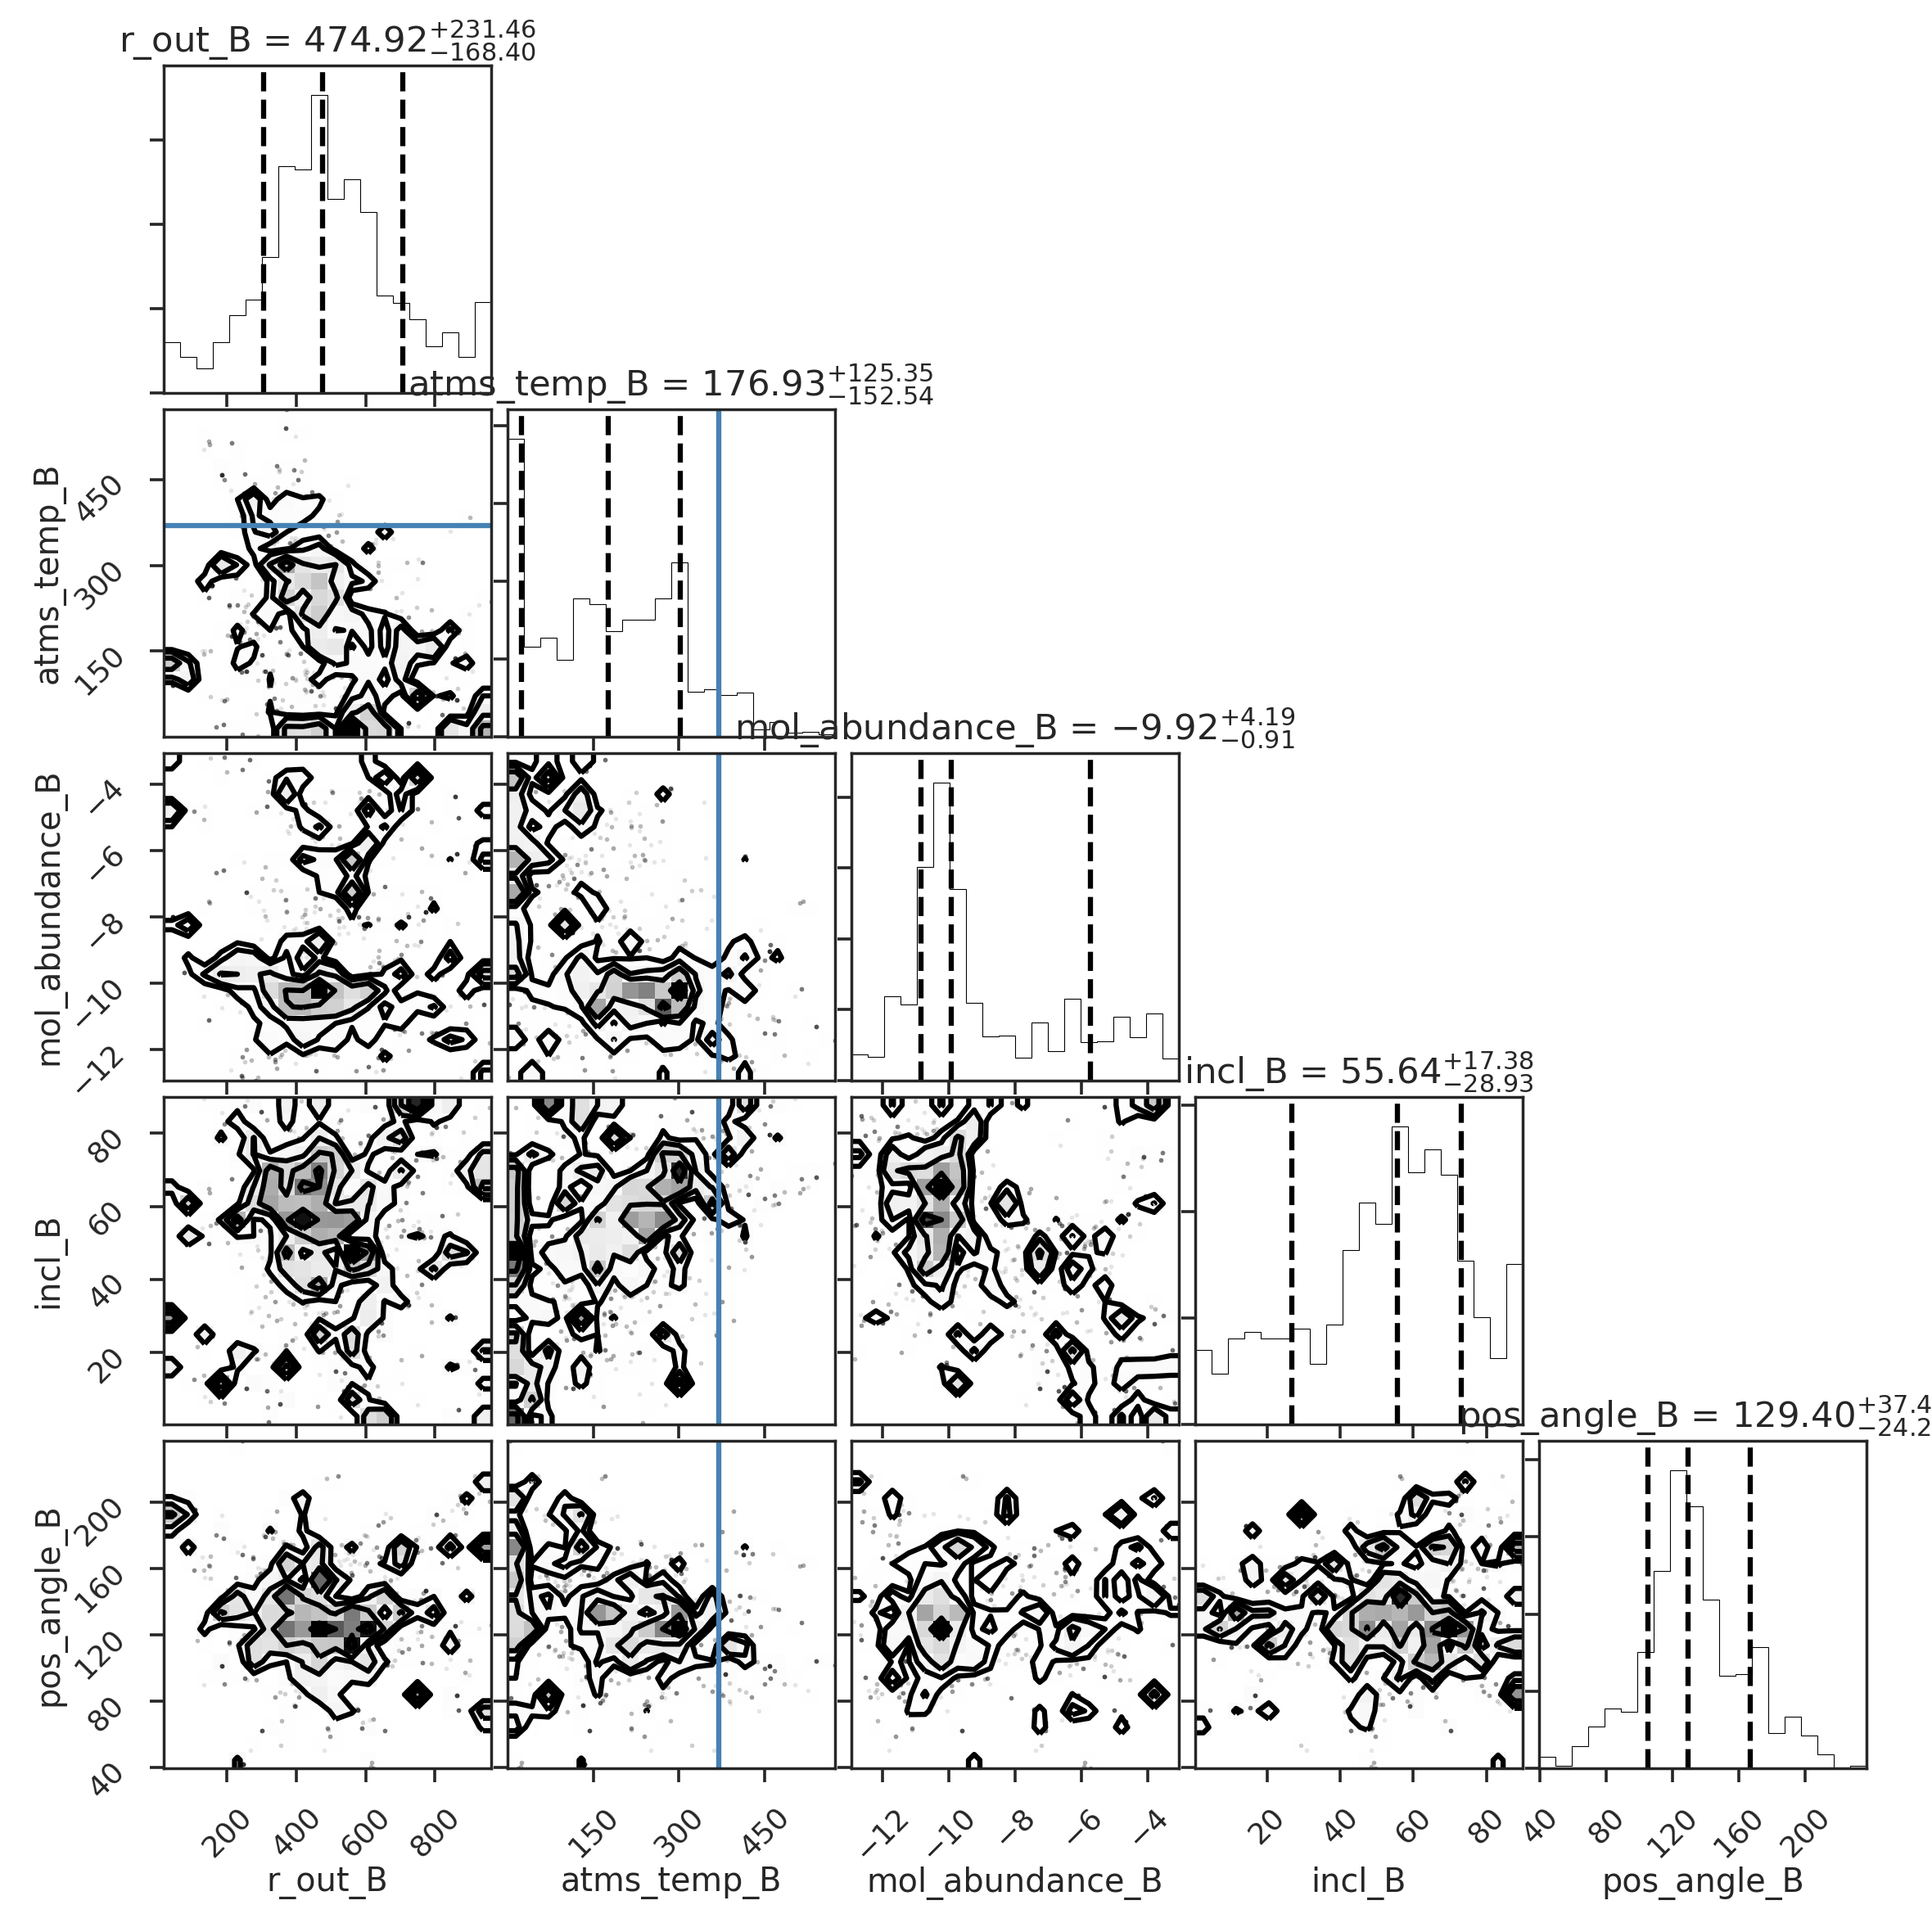
\includegraphics[width=0.49\linewidth]{cornerplot-diskB.png}}%
  \hspace*{\fill}%
  \caption{Since disk A and B's features are assumed to be independent, we may generate corner plots for each of their parameter spaces individually. Some analysis REWORK when new plots are added.}
  \label{fig:corner_plots}
\end{figure}





\section{Fitting Procedure}
\label{section:fitting_procedure}

Fitting of the data began with the analysis and partial removal of cloud contamination discussed in Section \ref{chap:results}, resulting in the removal of baselines below a characteristic length for each line. With the data as clean as possible, position ($\alpha, \delta$) and velocity ($v_\text{sys}$) offsets were fit for. Offset fitting was executed only in the HCO$^+$ line, thanks to the line's minimal contamination and high signal strength. To fit these offsets, all other disk parameters were fixed at hand-selected, ballpark-reasonable values and a grid search was run over RA/Dec offsets and systemic velocities for each disk, using grid resolutions that corresponded to our observation's spectro-spatial resolution. These grids were centered at values drawn from \cite{Williams2014}, where fits were made to the disks' continuum emission, but which proved to be in minor disagreement with our fitting. Positional offsets were confirmed with elliptical Gaussians in \texttt{CASA}. With these values established, they were treated as fixed parameters for the remainder of the fitting process.

% REWORK: Sam includes specific grid resolution and full disk coordinates. Maybe do that here, too.

Table \ref{table:fixed_params} presents a list of parameters, including $\alpha, \delta$, and $v_\text{sys}$, which were left fixed throughout the MCMC runs. Since we are only modeling one line at a time, we are unable to constrain the vertical temperature structure, and thus we fix T$_\text{mid}$ and $z_q$ (\cite{Factor2017}). Midplane temperature was drawn from \cite{Qi2011} to reproduce the midplane temperature structure and CO "snow line."


These parameters are generally either reasonably well-known in the literature (e.g. distance to the sources), or generally have small influences on flux magnitude and distribution relative to our observation's spectro-spatial resolution (e.g. turbulence velocity). Values for this second group drawn from previous studies of similar systems, or estimated based on theoretical considerations.


% If you are fixing a parameter, you should explain what value you assumed and why you left it fixed (usually either we have a constraint from some other observable, or it’s not well constrained by our data so we had to make a reasonable guess based on some previous study or theoretical consideration.  I think this section is at least as important as describing the parameters that you are fitting for!


\begin{table}
  \begin{threeparttable}
    \centering
    \caption{Fixed Parameter Values}
    \label{table:fixed_params}
    \renewcommand{\arraystretch}{1.2}
    \begin{tabular}{c  l  l  c  c }
      \toprule \toprule
      \multirow{2}{*}{Parameter} & \multirow{2}{*}{Description} & \multirow{2}{*}{Source} & \multicolumn{2}{c}{Fixed Value(s)} \\
                                 &                              &                         & (Disk A & Disk B) \\
      \midrule %\midrule
      $\Delta \alpha$ ($''$)       &  RA offset from image center     & Grid-search, elliptical fit & 0.0002 & -1.006  \\
      $\Delta \delta$ ($''$)       &  Dec offset from image center    & Grid-search, elliptical fit & 0.082  & -0.3 \\
      v$_\text{sys}$ (km s$^{-1}$) &  Systemic velocity               & Grid-search            & 10.00  & 10.75      \\
      M$_\star$ (M$_\odot$)        &  Stellar mass                    & \cite{Williams2014}    & 3.5    & 0.4   \\
      v$_\text{turb}$ (km s$^{-1}$ &  Turbulence velocity             & \cite{Flaherty2015}    & \multicolumn{2}{c}{0.081}   \\
      $d$ (pc)                     &  Distance                        & \cite{GaiaCollaboration2018} & \multicolumn{2}{c}{389}   \\
      R$_c$ (au)                   &  Critical radius                 & \cite{Williams2014}    & \multicolumn{2}{c}{100}\\
      $\gamma$                     &  Radial density power law index} & \cite{Andrews2009}    &  \multicolumn{2}{c}{1}\\
      $z_q$ (au)                   &  Disk scale height at 150 AU     & \cite{Factor2017}          & \multicolumn{2}{c}{29}\\
      T$_\text{mid}$ (K)           &  Midplane temperature at 150 AU  & \cite{Qi2011}          & \multicolumn{2}{c}{19}\\
      \bottomrule
    \end{tabular}

    \begin{tablenotes}\footnotesize
      \item[a] Fit with grid search.
      \item[d] Values used by \cite{Flaherty2015} for modeling HD 163296.
      \item[e] Retrieved from \cite{Williams2014}
    \end{tablenotes}
  \end{threeparttable}
\end{table}


The remaining parameters, presented and discussed in \ref{table:fit_params}, are fit for using MCMC. We implement priors on each parameter, reported in Table \ref{table:fit_priors}. Gaussian priors are used for the fitting of both disks' position angles, centered at values presented by \cite{Williams2014}, but which we would like to improve upon.

\begin{table}
  \begin{threeparttable}
    \centering
    \caption{Fit Parameter Values}
    \label{table:fit_priors}
    \renewcommand{\arraystretch}{1.2}
    \begin{tabular}{c  l l }
      \toprule \toprule
      Parameter             &  Description                                     & Prior   \\
      \midrule %\midrule
      $i$ ($^o$)            &  Inclination\tnote{a}                            & Uniform  \\
      $PA$ ($^o$)           &  Position Angle                                  & Gaussian \\
      X$_\text{mol}$        &  Molecular abundance, relative to H$_2$\tnote{b} & Uniform \\
      $q$                   &  Radial temperature power law index              & Uniform \\
      T$_\text{atms}$ (K)   & Atmosopheric temperature at 150 AU               & Uniform \\
      M$_\text{Disk}$ (M$_\odot$) &  Log Disk mass\tnote{c}                    & Log Uniform \\
      \bottomrule
    \end{tabular}

    \begin{tablenotes}\footnotesize
      \item[a] Since disk B is unresolved, we fix $i_B = 45$.
      \item[b] For the CO line, X$_\text{mol}$ is fixed at the literature value of $10^{-4}$.
      \item[c] For HCO$^+$(4-3), HCN, and CS, disk mass was fixed at values from \cite{Williams2014}.
    \end{tablenotes}
  \end{threeparttable}
\end{table}


The result from the MCMC runs are presented below.





\subsection{CO (3-2) Fit}
We began by fitting the CO line. Since we fix CO's relative molecular abundance at X$_\text{mol}=10^{-4}$, we may directly fit for the disks' masses and then use those values for the other lines.

The significant cloud contamination in the CO line presents difficulties for fitting. Since the contamination is most significant in the central five channels, those channels were not included in the fitting process. Although this degrades the

Additionally, maybe a tidal feature. Best fit values are reported in Table \ref{table:fit_co}



\begin{table}
  \begin{threeparttable}
    \centering
    \caption{MCMC Fitting Results (CO)}
    \label{table:fit_co}
    \renewcommand{\arraystretch}{1.2}
    \begin{tabular}{c c l c l }
      \toprule \toprule
      %\multirow{2}{*}{Parameter} & \multirow{2}{*}{Disk A}    & \multicolumn{2}{c}{Disk B} \\
      \multirow{2}{*}{Parameter} & \multicolumn{2}{c}{Disk A} & \multicolumn{2}{c}{Disk B} \\
                                 & Median & Best Fit          & Median & Best Fit \\
      \midrule %\midrule
      $\log M_\text{Disk}$ (M$_\odot$) & $ -n _{-0.} ^{+0.}$ & $-0.29$    & $ -n _{-0.} ^{+0.}$ & $-4.9$ \\
      $r_{out}$(\si{au})               & $ -n _{-0.} ^{+0.}$ & $437.71$    & $ -n _{-0.} ^{+0.}$  & $261.13$    \\
      $i$ (\si{\degree})               & $ -n _{-0.} ^{+0.}$ & $65$    & $ -n _{-0.} ^{+0.}$ & $45$    \\
      PA  (\si{\degree})               & $ -n _{-0.} ^{+0.}$ & $66.73$  & $ -n _{-0.} ^{+0.}$  & $[136]$  \\
      q                                & $ -n _{-0.} ^{+0.}$ & $0.28$  & $ -n _{-0.} ^{+0.}$  & $[-0.5]$  \\
      T$_\text{atms}$ (K)              & $ -n _{-0.} ^{+0.}$ & $5.54 $  & $ -n _{-0.} ^{+0.}$  & $177.15$  \\
      $\ln$ Likelihood          & \multicolumn{4}{c}{$-33597.46$} \\
      \bottomrule
    \end{tabular}

    \begin{tablenotes}\footnotesize
      \item[*] Values in [brackets] were fixed for this run.
    \end{tablenotes}
  \end{threeparttable}
\end{table}




\subsection{HCO$^+$ (4-3) Fit}

\begin{table}
  \begin{threeparttable}
    \centering
    \caption{MCMC Fitting Results (HO$^+$)}
    \label{table:fit_hco}
    \renewcommand{\arraystretch}{1.2}
    \begin{tabular}{c c l c l }
      \toprule \toprule
      %\multirow{2}{*}{Parameter} & \multirow{2}{*}{Disk A}    & \multicolumn{2}{c}{Disk B} \\
      \multirow{2}{*}{Parameter} & \multicolumn{2}{c}{Disk A} & \multicolumn{2}{c}{Disk B} \\
                                 & Median & Best Fit          & Median & Best Fit \\
      \midrule %\midrule
      X$_\text{mol}$             & $ -n _{-0.} ^{+0.}$ & $-8.18$    & $ -n _{-0.} ^{+0.}$ & $-9.86$ \\
      $r_{out}$(\si{au})        & $ -n _{-0.} ^{+0.}$ & $330.86$    & $ -n _{-0.} ^{+0.}$  & $147.69$    \\
      $i$ (\si{\degree})        & $ -n _{-0.} ^{+0.}$ & $65$    & $ -n _{-0.} ^{+0.}$ & $45$    \\
      PA  (\si{\degree})        & $ -n _{-0.} ^{+0.}$ & $[66.73]$  & $ -n _{-0.} ^{+0.}$  & $[112.94]$  \\
      q                         & $ -n _{-0.} ^{+0.}$ & $0.77$  & $ -n _{-0.} ^{+0.}$  & $[-0.5]$  \\
      T$_\text{atms}$ (\si{\K}) & $ -n _{-0.} ^{+0.}$ & $172.95 $  & $ -n _{-0.} ^{+0.}$  & $186.17$  \\
      $\ln$ Likelihood          & \multicolumn{4}{c}{$-28395.97$} \\
      \bottomrule
    \end{tabular}
    \begin{tablenotes}\footnotesize
      \item[*] Values in [brackets] were fixed for this run.
    \end{tablenotes}
  \end{threeparttable}
\end{table}









\subsection{HCN (4-3) Fit}
Starting with HCN to get disk mass.

Best fit values are reported in Table \ref{table:fit_hcn}


\begin{table}
  \begin{threeparttable}
    \centering
    \caption{MCMC Fitting Results (HCN)}
    \label{table:fit_hcn}
    \renewcommand{\arraystretch}{1.2}
    \begin{tabular}{c c l c l }
      \toprule \toprule
      %\multirow{2}{*}{Parameter} & \multirow{2}{*}{Disk A}    & \multicolumn{2}{c}{Disk B} \\
      \multirow{2}{*}{Parameter} & \multicolumn{2}{c}{Disk A} & \multicolumn{2}{c}{Disk B} \\
                                 & Median & Best Fit          & Median & Best Fit \\
      \midrule %\midrule
      X$_\text{mol}$             & $ -n _{-0.} ^{+0.}$ & $-7.87$    & $ -n _{-0.} ^{+0.}$ & $-11.09$ \\
      $r_{out}$(\si{au})        & $ -n _{-0.} ^{+0.}$ & $334.48$    & $ -n _{-0.} ^{+0.}$  & $221.37$    \\
      $i$ (\si{\degree})        & $ -n _{-0.} ^{+0.}$ & $65$    & $ -n _{-0.} ^{+0.}$ & $45$    \\
      PA  (\si{\degree})        & $ -n _{-0.} ^{+0.}$ & $69.26$  & $ -n _{-0.} ^{+0.}$  & $138.2$  \\
      q                         & $ -n _{-0.} ^{+0.}$ & $0.62$  & $ -n _{-0.} ^{+0.}$  & $[-0.5]$  \\
      T$_\text{atms}$ (\si{\K}) & $ -n _{-0.} ^{+0.}$ & $125.68 $  & $ -n _{-0.} ^{+0.}$  & $388.21$  \\
      $\ln$ Likelihood          & \multicolumn{4}{c}{$-30928.35$} \\
      \bottomrule
    \end{tabular}
    \begin{tablenotes}\footnotesize
      \item[*] Values in [brackets] were fixed for this run.
    \end{tablenotes}
  \end{threeparttable}
\end{table}


% % REWORK: Didn't actually fit for incl. Change the tables.










%% ~~~~ FIGURES ~~~~~~~~~~~~~~~~~~~~~~~~~~~~~~~~~~~~~~~~~~~~~~~~~~~~~~~~~~~~~~~~



%% ~~~ CO ~~~~~~~~~~~~~~~~~~~~~~~~~~~~~~~~~~~~~~~~~~~~~~~~~~~~~~~~~~~~~~~~~~~~~~

\begin{figure}[htp]
  \hspace*{\fill}%
  \subcaptionbox{Disk A fits \label{fig:corner_a}}{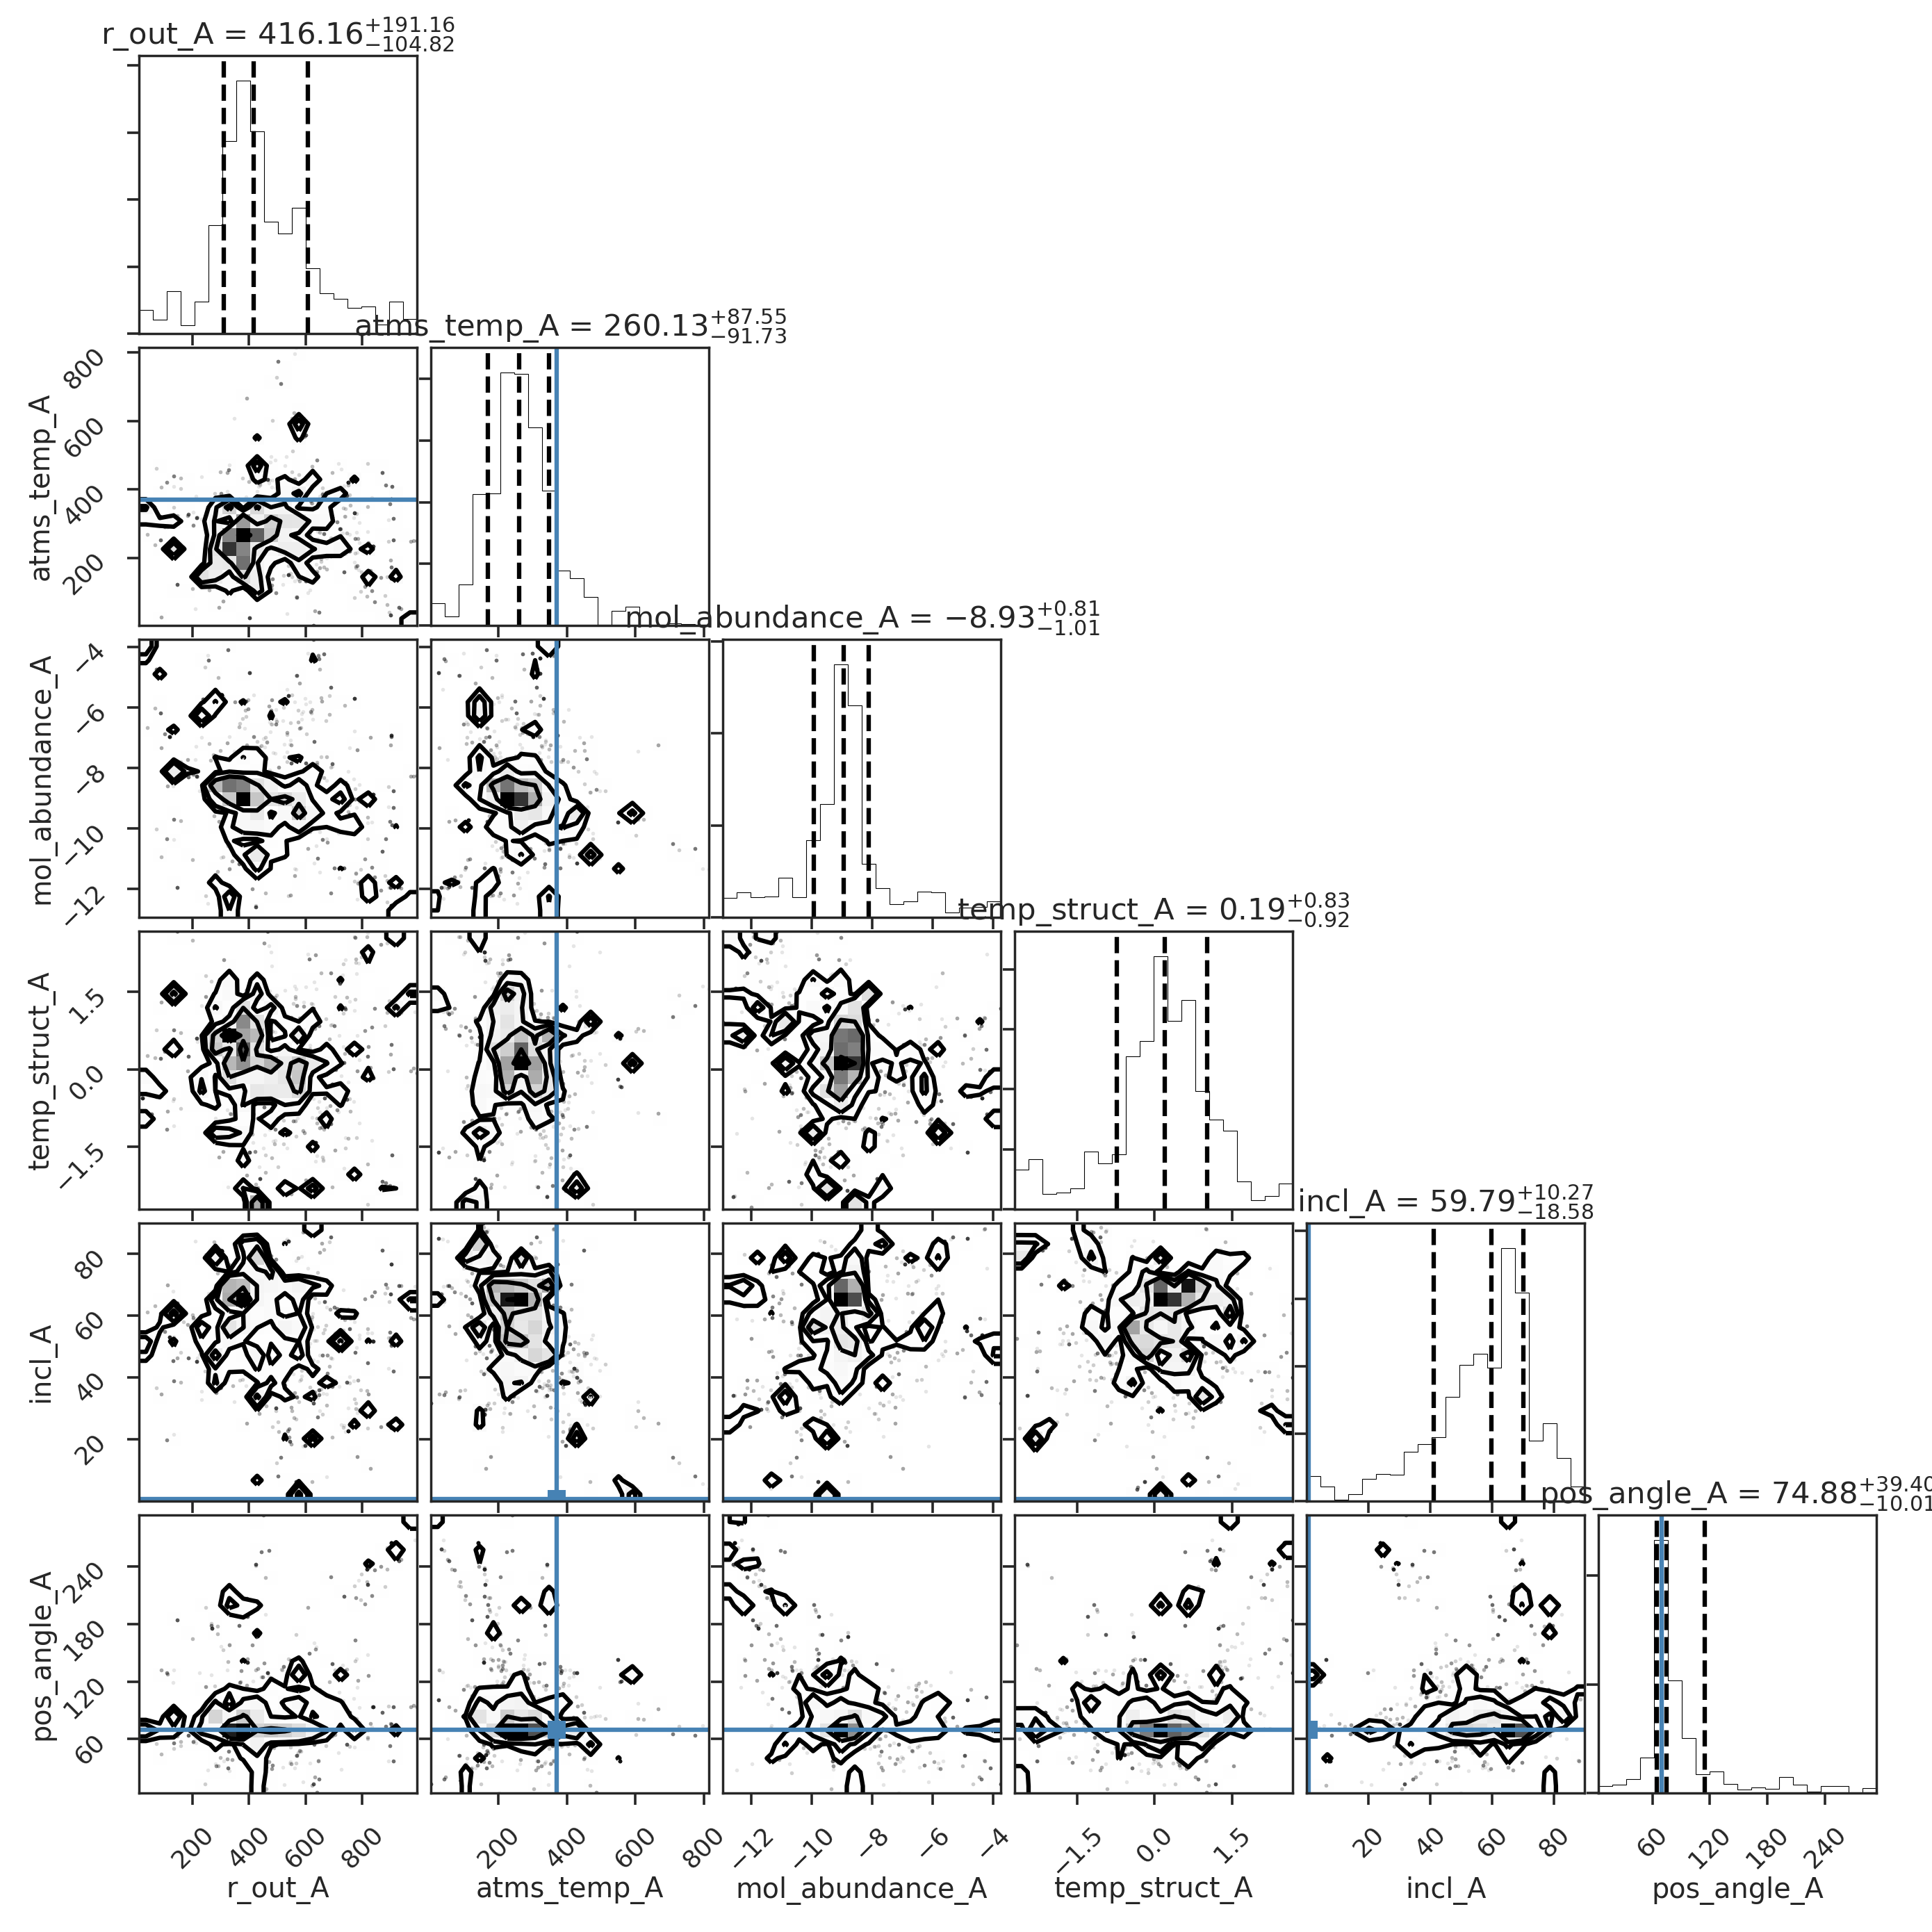
\includegraphics[width=0.49\linewidth]{cornerplot-diskA.png}}\hfill%
  \subcaptionbox{Disk B fits \label{fig:corner_b}}{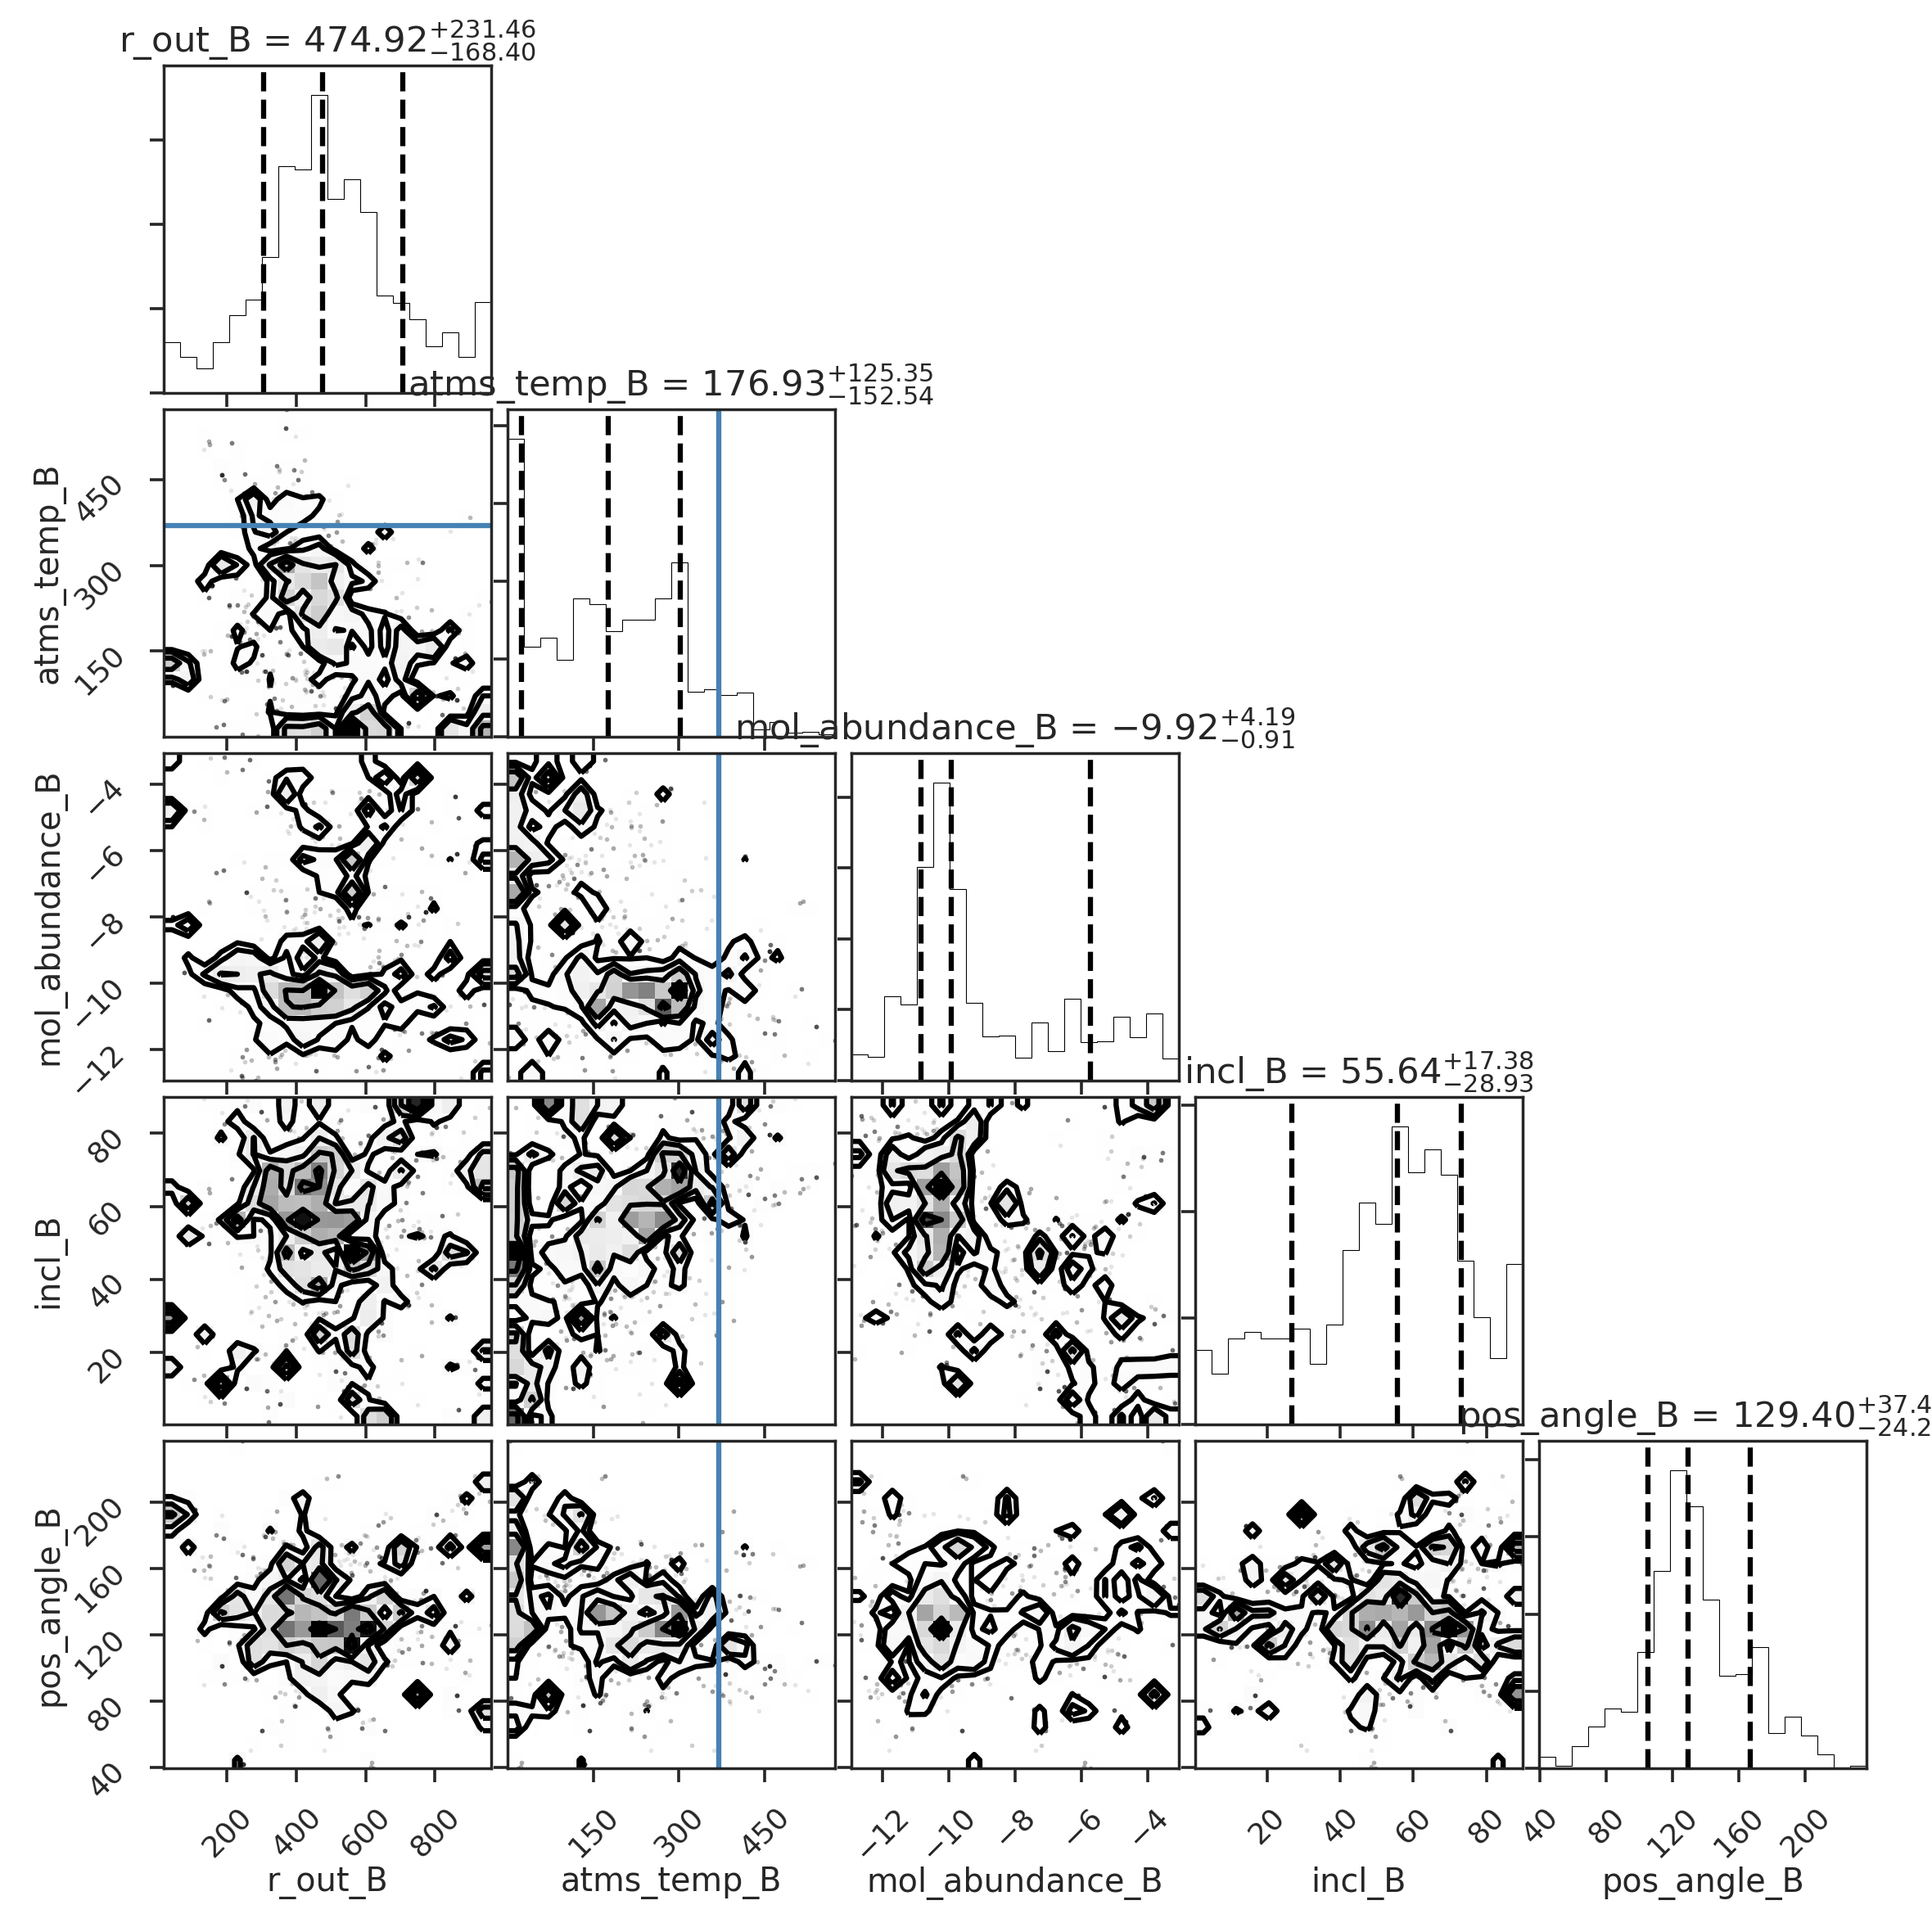
\includegraphics[width=0.49\linewidth]{cornerplot-diskB.png}}%
  \hspace*{\fill}%
  \caption{Since disk A and B's features are assumed to be independent, we may generate corner plots for each of their parameter spaces individually. Some analysis REWORK when new plots are added.}
  \label{fig:co_corner_plots}
\end{figure}


\begin{figure}[htp]
  \hspace*{\fill}%
  \includegraphics[width=\linewidth]{chanmaps-co.pdf}\hfill%
  \hspace*{\fill}%
  \caption{Since disk A and B's features are assumed to be independent, we may generate corner plots for each of their parameter spaces individually. Some analysis REWORK when new plots are added.}
  \label{fig:co_chanmaps}
\end{figure}



%% ~~~ HCO ~~~~~~~~~~~~~~~~~~~~~~~~~~~~~~~~~~~~~~~~~~~~~~~~~~~~~~~~~~~~~~~~~~~~~

\begin{figure}[htp]
  \hspace*{\fill}%
  \subcaptionbox{Disk A fits \label{fig:corner_a}}{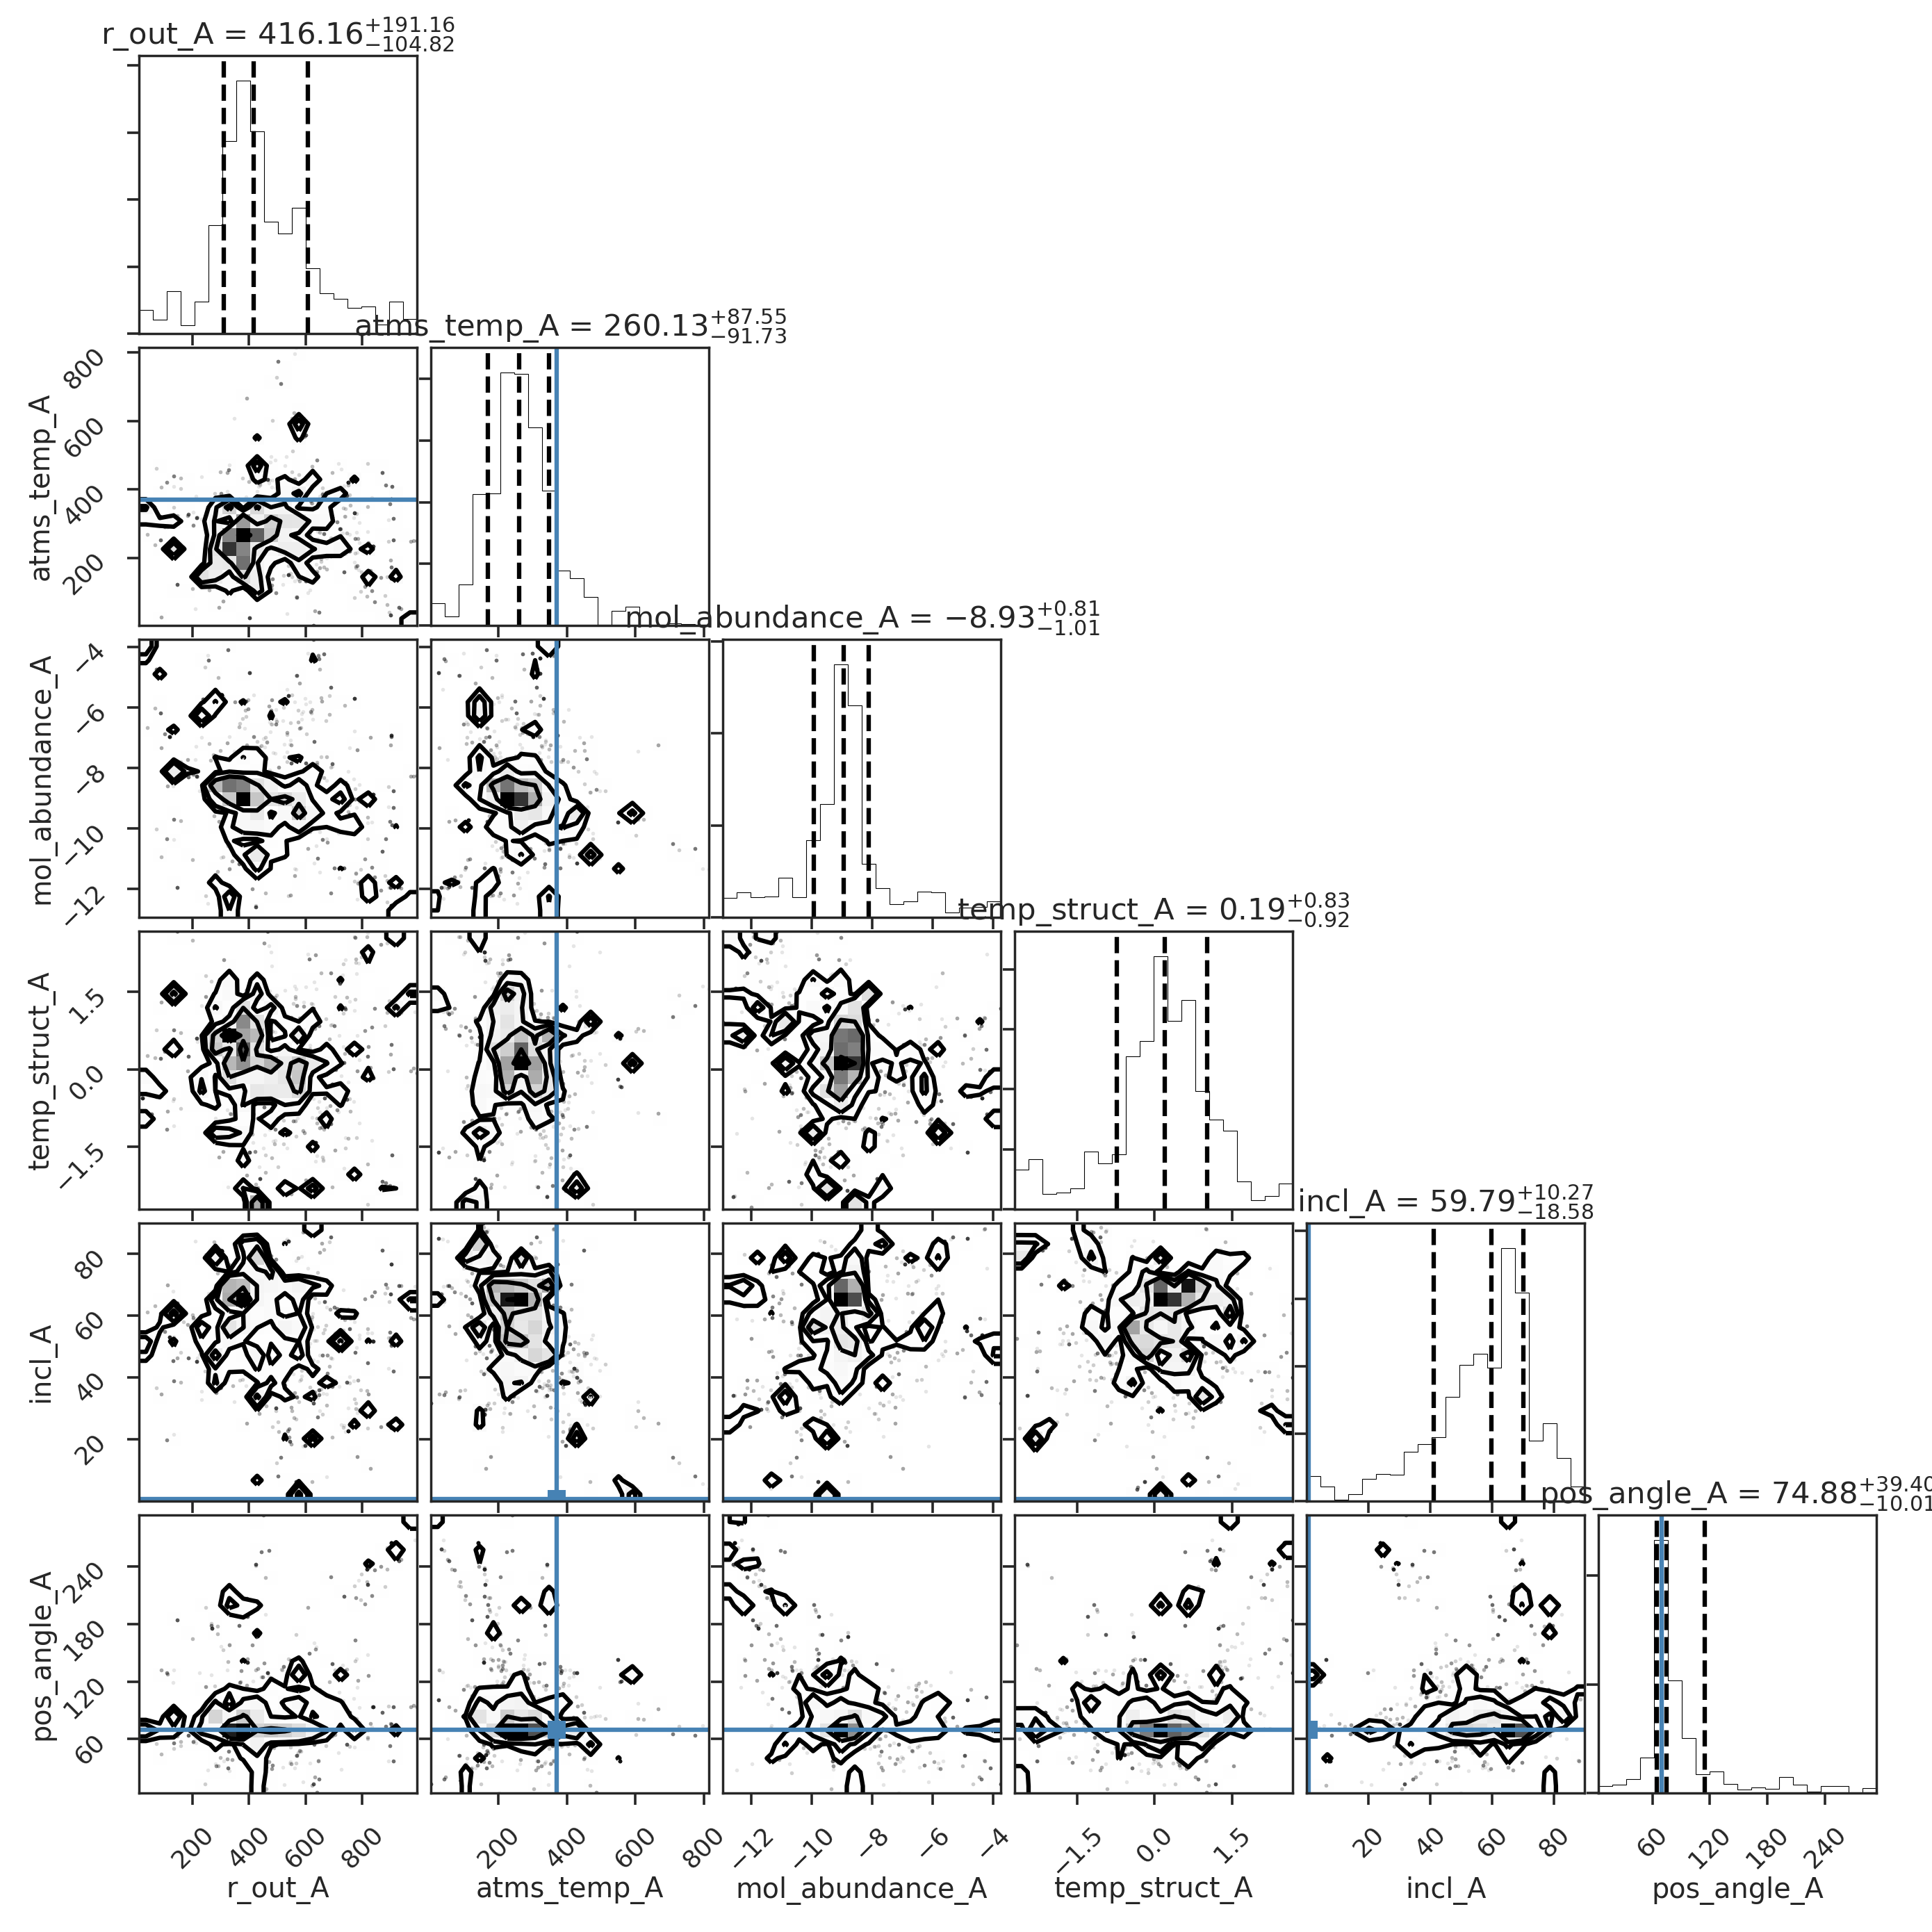
\includegraphics[width=0.49\linewidth]{cornerplot-diskA.png}}\hfill%
  \subcaptionbox{Disk B fits \label{fig:corner_b}}{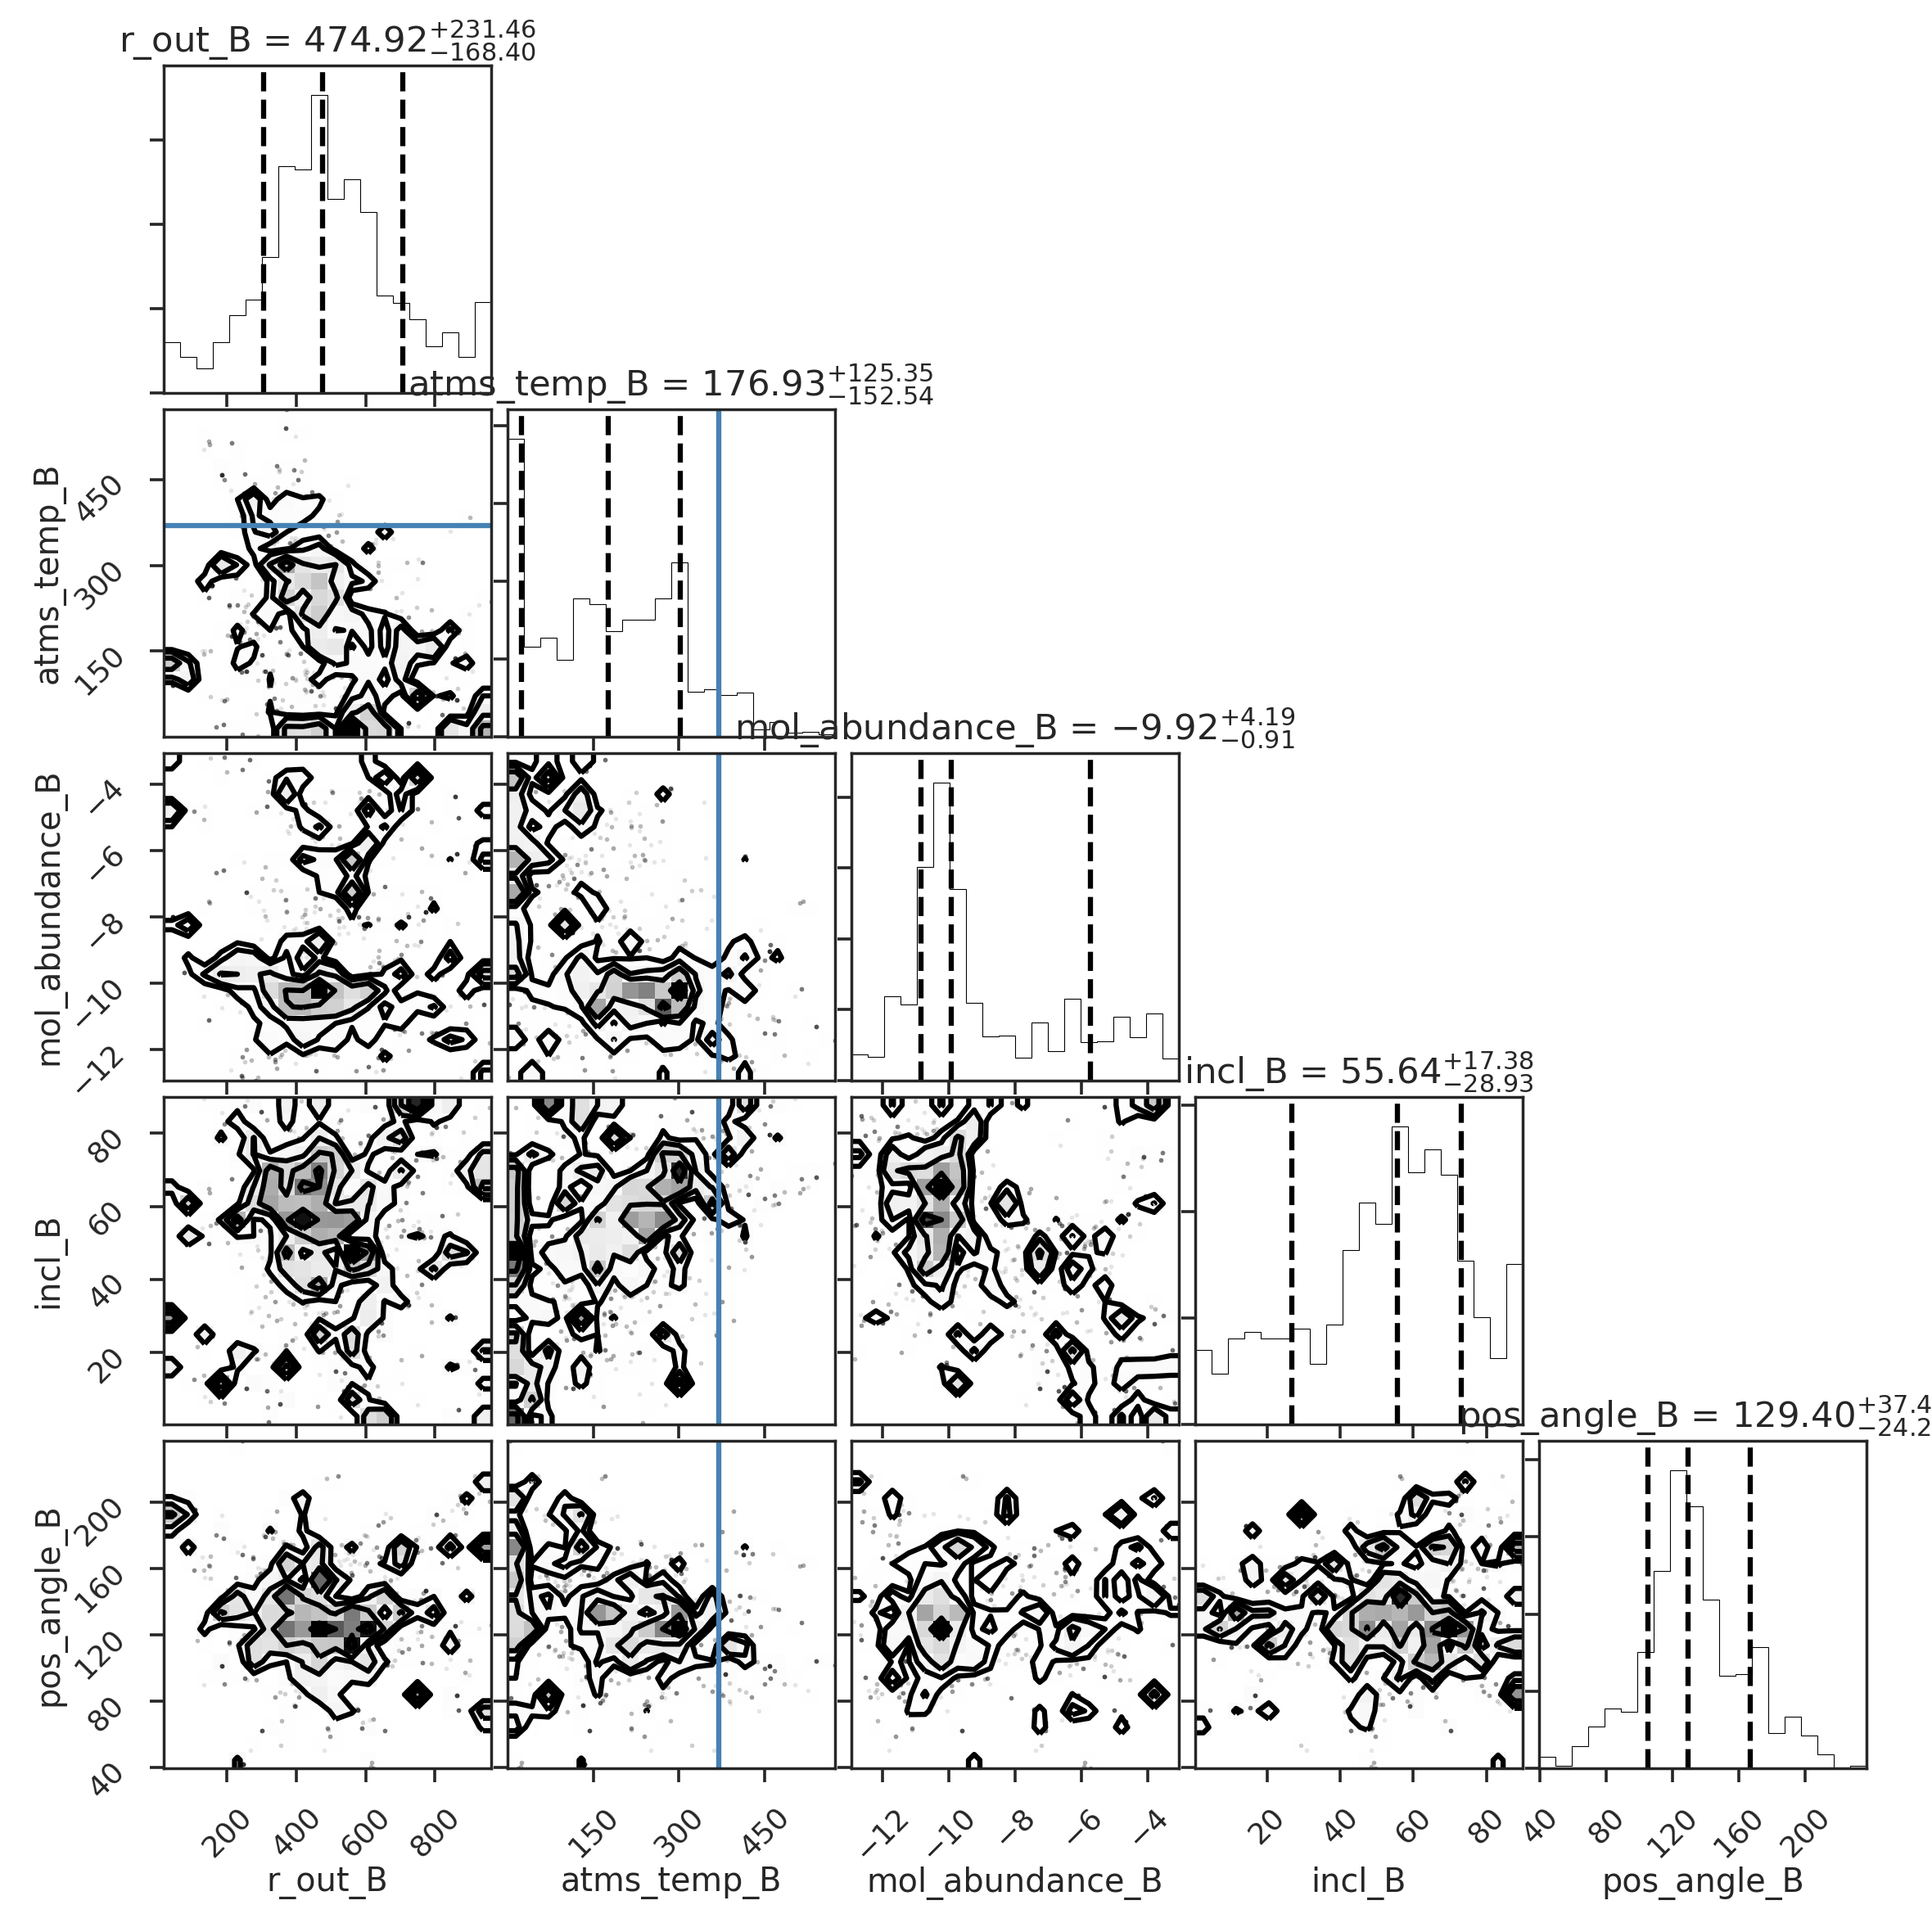
\includegraphics[width=0.49\linewidth]{cornerplot-diskB.png}}%
  \hspace*{\fill}%
  \caption{Since disk A and B's features are assumed to be independent, we may generate corner plots for each of their parameter spaces individually. Some analysis REWORK when new plots are added.}
  \label{fig:co_corner_plots}
\end{figure}


\begin{figure}[htp]
  \hspace*{\fill}%
  \includegraphics[width=\linewidth]{chanmaps-hco.pdf}\hfill%
  \hspace*{\fill}%
  \caption{Data, model, and residual maps are presented.}
  \label{fig:co_chanmaps}
\end{figure}


%% ~~~ HCN ~~~~~~~~~~~~~~~~~~~~~~~~~~~~~~~~~~~~~~~~~~~~~~~~~~~~~~~~~~~~~~~~~~~~~

\begin{figure}[htp]
  \hspace*{\fill}%
  \subcaptionbox{Disk A fits \label{fig:corner_a}}{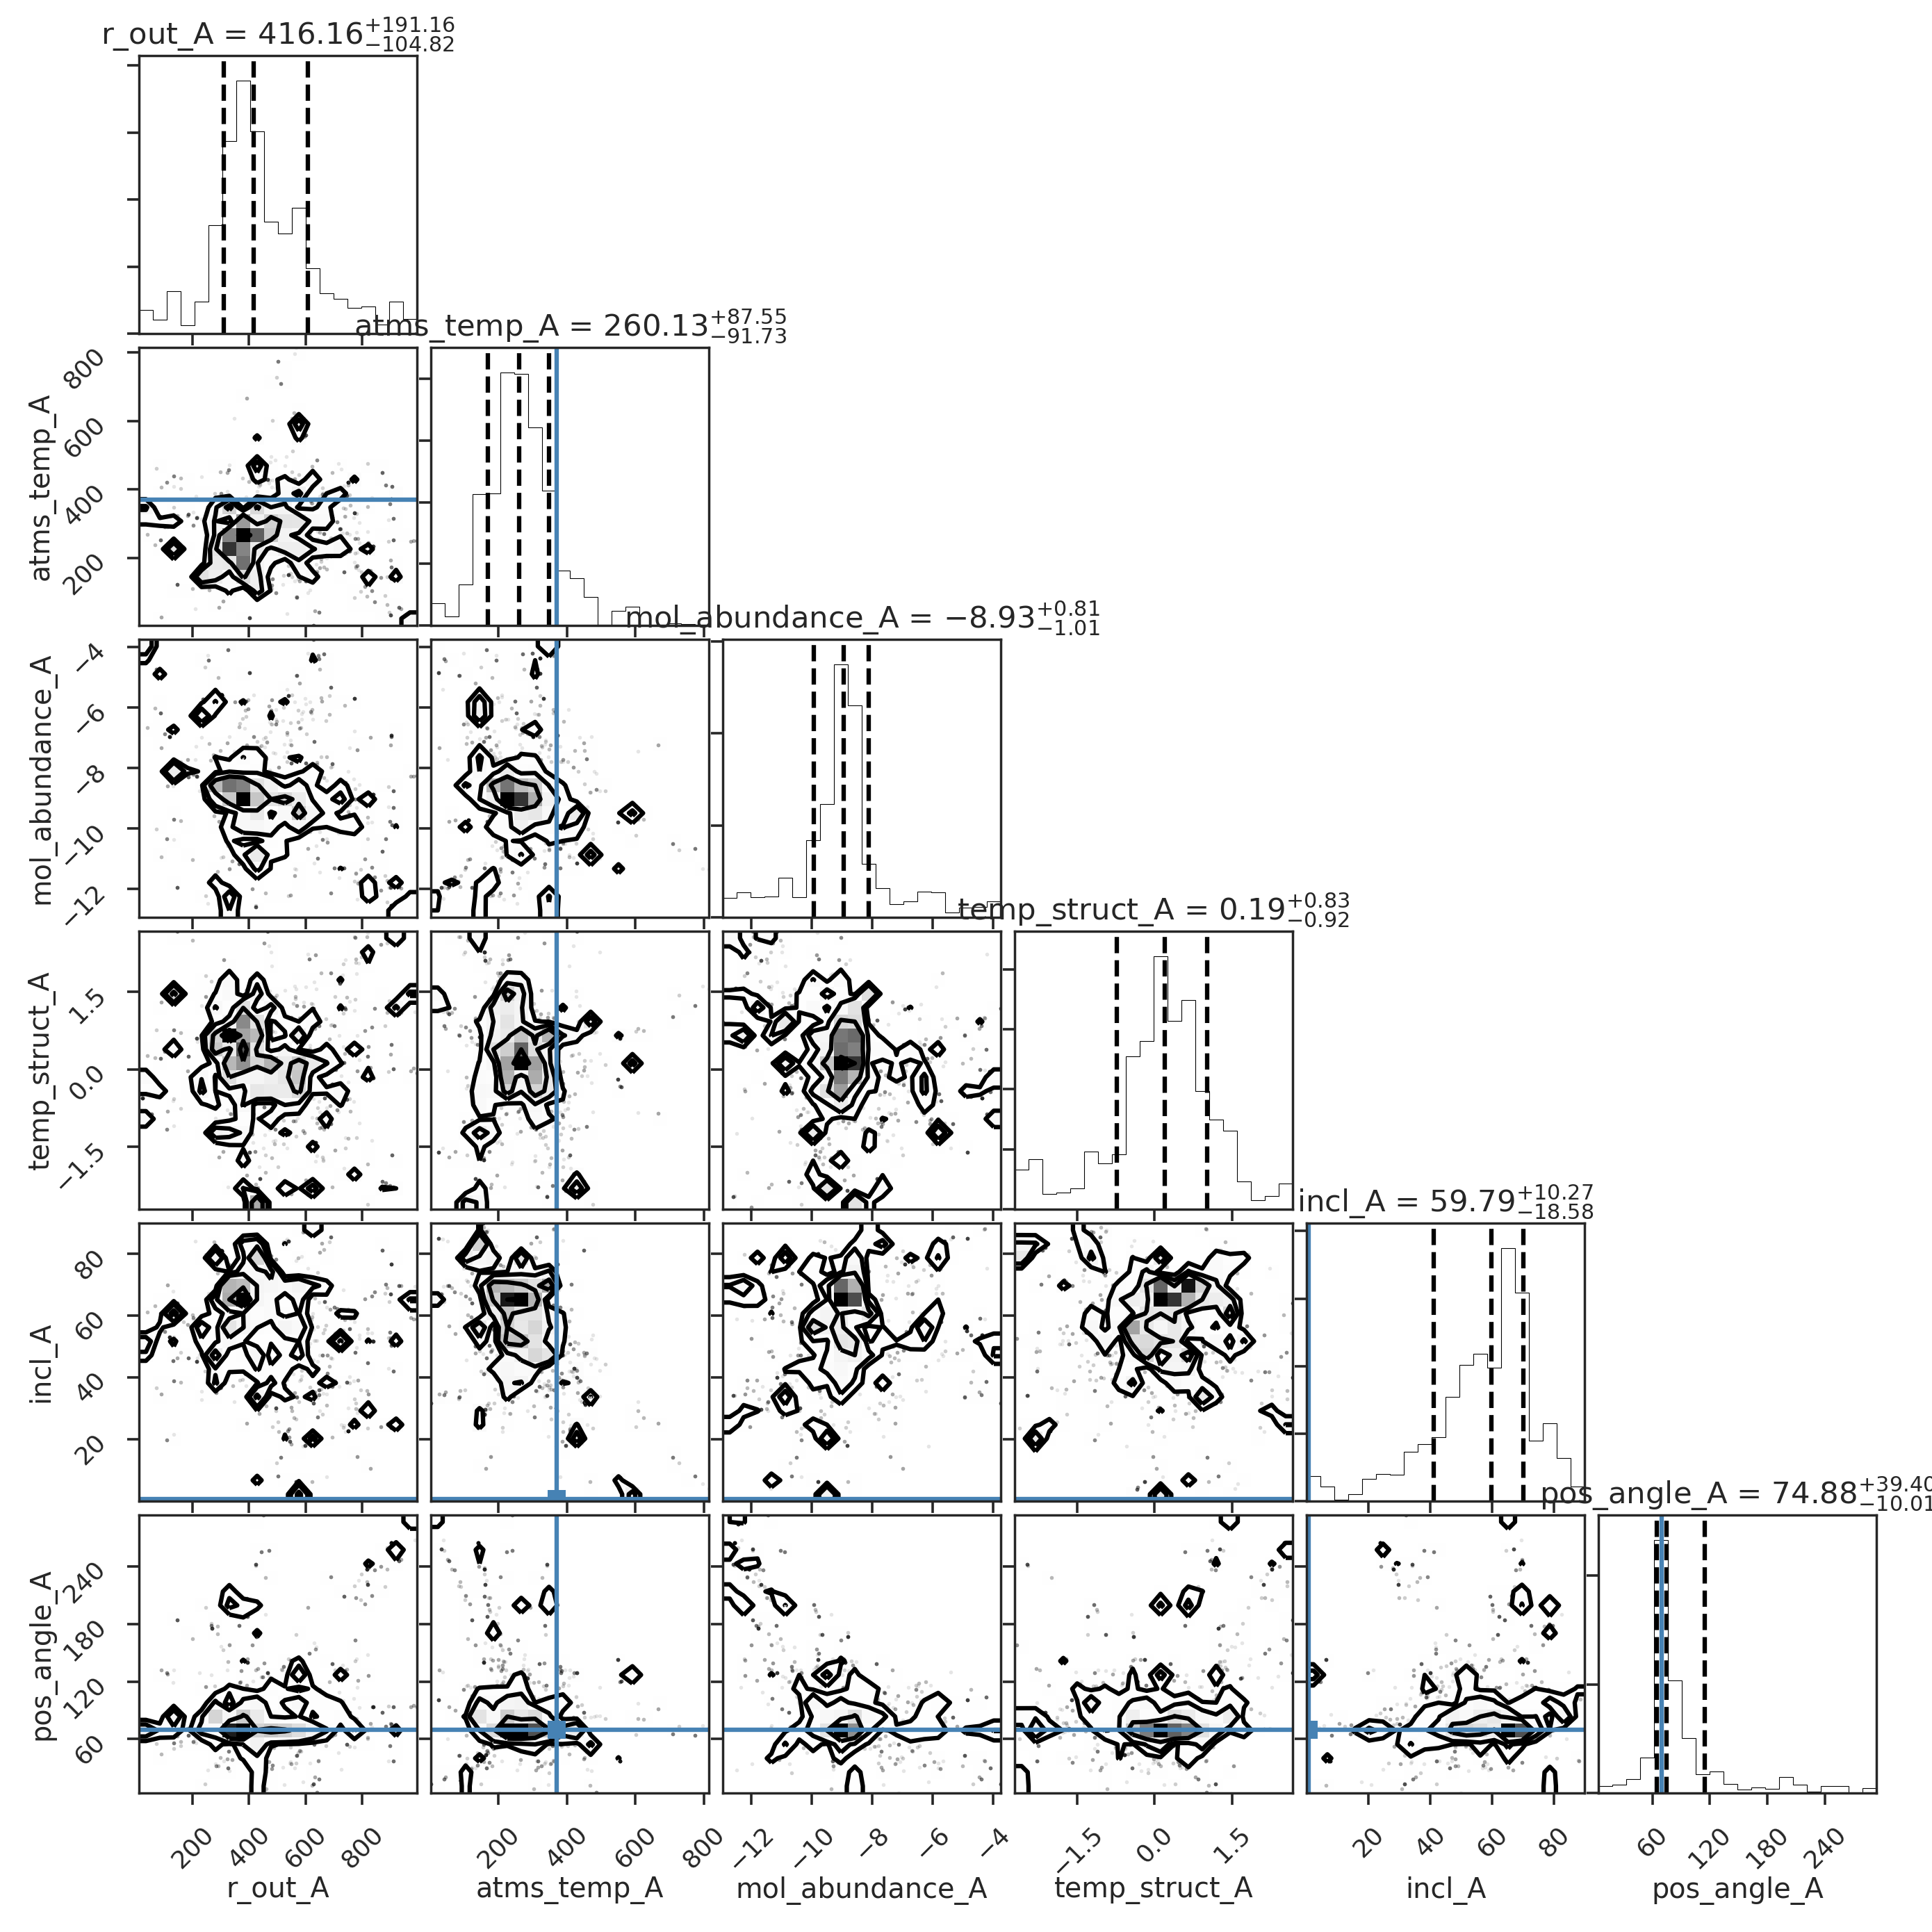
\includegraphics[width=0.49\linewidth]{cornerplot-diskA.png}} \hfill%
  \subcaptionbox{Disk B fits \label{fig:corner_b}}{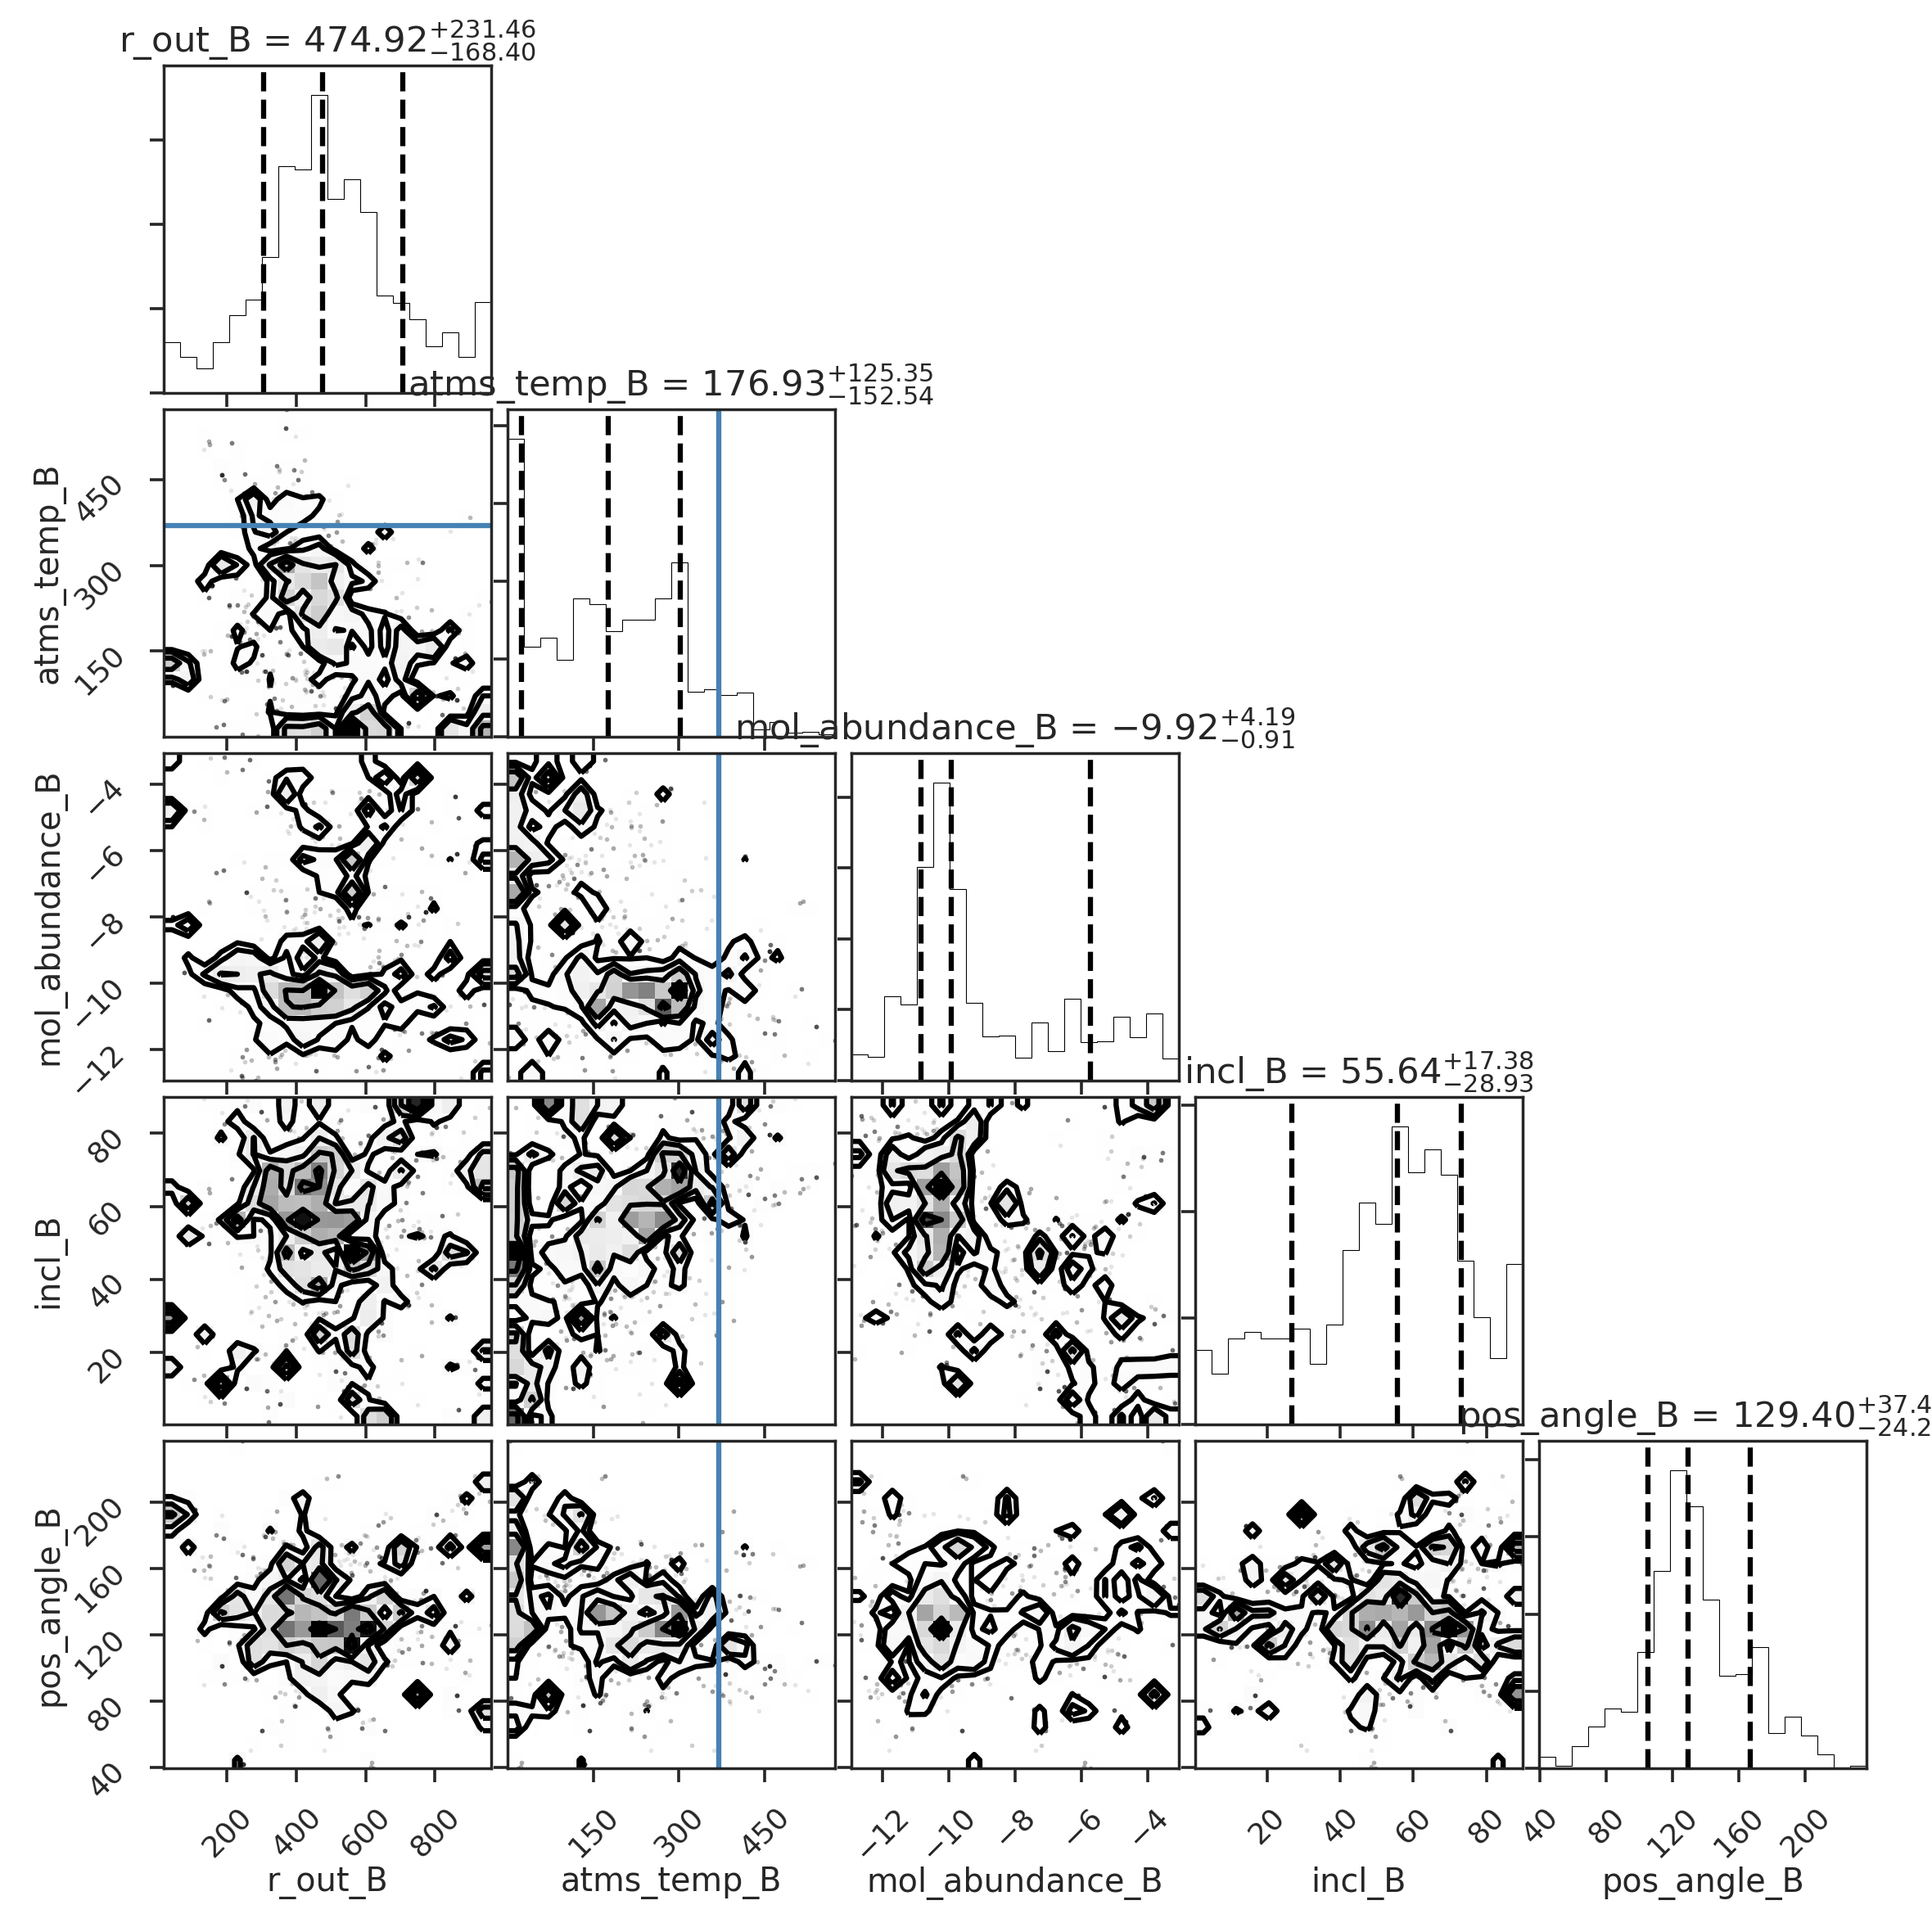
\includegraphics[width=0.49\linewidth]{cornerplot-diskB.png}}%
  \hspace*{\fill}%
  \caption{Since disk A and B's features are assumed to be independent, we may generate corner plots for each of their parameter spaces individually. Some analysis REWORK when new plots are added.}
  \label{fig:co_corner_plots}
\end{figure}


\begin{figure}[htp]
  \hspace*{\fill}%
  \includegraphics[width=\linewidth]{march26_DMR-images.pdf}\hfill%
  \hspace*{\fill}%
  \caption{Since disk A and B's features are assumed to be independent, we may generate corner plots for each of their parameter spaces individually. Some analysis REWORK when new plots are added.}
  \label{fig:co_chanmaps}
\end{figure}





% \begin{itemize}
%   \item \textsc{RA/Dec Offsets} ($\Delta \delta, \Delta \alpha$): The positional offsets from image center for each disk, in arc-seconds. Originally fit with a Gaussian centroid, these offsets were validated/refined with a narrow-range grid search.
%   \item \textsc{Systemic Velocity} (v$_{\text{sys}}$): The radial velocity of each disk, in km s$^{-1}$. Initialized at values drawn from \cite{Williams2014}, these were also validated/refined using a narrow-range grid search.
%   \item \textsc{Distance} ($d$): The distance to the sources, in parsecs. Drawn from Gaia DR2 catalogue.
%   \item \textsc{Inner Radius} ($r_\text{in}$): Each disk's inner radius. Since these disks show no evidence of their interiors being carved out, we do not fit for an interior ring and allow the disks to extend almost all the way in to their stars.
%   \item \textsc{Turbulence Velocity} ($v_{\text{turb}}$): The speed of the turbulence in the disk. This value was left at its default, which \textit{maybe came from Flaherty}
%   \item \textsc{Vertical Temp. Str. Scale Height} ($Z_q$): The characteristic height, set at $r=150$ AU, determining the vertical temperature structure.
%   \item \textsc{Column Densities ([min, max])} ($[\sigma_1, \sigma_2]$): Min and max column density boundaries (corresponding to upper and lower boundaries) of molecular zone, in units of 1.59$\times10^{21}$ particles cm$^{-2}$
%   \item \textsc{Freeze-out Temperature} (T$_\text{FO}$): \textit{Wait why is this never used in my code.}
%   \item \textsc{Stellar Mass} (M$_\star$):
%   % \item \textsc{x} (y):
% \end{itemize}



% The End

\chapter{Discussion}
\label{chap:discussion}

With the disks now fit, we may interpret our results. Since this project was based on the question of how environment influences protoplanetary disks, we would like to compare the best fit values (with consideration given to their associated uncertainties) to the values found by \citet{Factor2017}, to those found through line-emission observations of other systems, and to those derived from modeling. We also view our results in the context of planet formation potential, and maybe discuss some other stuff, too.


\section{Reflections on the Fits}

It's nice to see that HCN and \hco agree so well. Almost weird how well they agree on abundance.

CO got trapped in a bad local min. Either try chopping that or just give up on it.

disk B is probably too wonky to fit? HCN just straight up didn't converge, which is probably because of disk B, and \hco has such a comically high temperature that it seems like it must be wrong. Cool (and, again, weird) to see that they agree so well on the abundance. Could reflect the fixed $q = -0.5$ maybe?



It is (maybe?) possible that my consistently positive $q$ values reflect the fact that our fits had different values for some of the fixed parameters. These include R$_{crit}$, which we fix at 100 and Sam fixed at 600 AU, as well as $z_q$ and $T_\text{mid}$, which Sam fit for and which together control how the temperature structure decays vertically (see \S\ref{subsection:physical_profs} for a more complete description). Since Sam fit multiple lines simultaneously, they were able to constrain these parameters, which is not possible in the case of single-line fitting. In a CO and \hco fit, they found values of $z_{q, 150} = 73$ AU and T$_{mid} = 24.7$ K, in comparison to our values of 29 and 19, respectively. \textit{Is this enough to make an appreciable difference? I don't know. It seems most likely to me that those drastically different R$_C$ values could explain the different q values, since if my disks are having their densities killed way earlier, then maybe they're struggling to match the flux levels further out. }

\textit{Another question about Sam's work: His paper and thesis have different values for the \hco and CO fits. He also makes no mention of the multi-line fits in his paper, which seems weird.}




This seems consistent with the hypothesis, based on the wide separation of the binary's components, that these disks may have formed separately, in regions with different chemistries, and drifted together later. Maybe?

\citet{Williams2014} note that previous works on wide binaries \citep{JensenAkeson2014,Salyk2014} have indicated that these pairs likely do not form together in the same large, co-rotating structures.


The HCN line chanmaps show a really strong conection between disks around v=10.24, 9.83. Maybe it's just disk B reappearing, but the connector seems a lot stronger in this line than in HCO+. Does this reflect their different emitting regions?


\section{Comparison with the Literature}

\cite{table:comparisons} we compare our results to those from other studies that have modeled line emission from protoplanetary disks. The most immediately relevant of these is the work by \citet{Factor2017}, in which they use a similar modeling technique to characterize another ONC proplyd from the same survey as our binary, and thus represent the only other disk studied in this way that is also in a high-mass star forming region. The others are well-studied disks in low-mass regions. We may compare our temperature profiles and abundance to these other systems and look for variations from expected values.


\begin{table}
  \centering
  \begin{threeparttable}
    \caption{Best-fit Results from \citet{Factor2017}}
    \label{table:comparisons}
    \renewcommand{\arraystretch}{1.2}
    \begin{tabular}{l l l c c c }
      \toprule \toprule
      %\multirow{2}{*}{Parameter} & \multirow{2}{*}{Disk A}    & \multicolumn{2}{c}{Disk B} \\
      Reference                             & Source     & Line      & $q$   & log X$_\text{mol}$ & Atms. Temp\\
      \midrule %\midrule
      \multirow{3}{*}{This study}}          & d253-1536a & \hco(4-3)      & 0.66  & -7.96         & 151  \\
                                            & d253-1536a & HCN(4-3)       & 0.72  & -7.62         & 140  \\
                                            & d253-1536a & CO(3-2)\tnote{a} & 0.40  & [-4]        & 1  \\
      \hline
      \multirow{3}{*}{\citet{Factor2017}}   & d216-0939  & \hco(4-3)      & 0.17  & -10.08        & 190  \\
                                            & d216-0939  & CO(3-2)        & -0.33 & [-4]          & 70  \\
                                            & d216-0939  & HCN(4-3)       & -0.18 & -6.7          & 19  \\
      \hline
      \multirow{2}{*}{\citet{Flaherty2015}} & HD163296   & CO(3-2)        & -0.22 & [-4]          & 94  \\
                                            & HD163296   & CO(2-1)        & -0.27 & [-4]          & 79  \\
      \hline
      \citet{Rosenfeld2012}\tnote{a}        & V4046 Sgr  & $^{12}$CO(2-1) & 0.63 & [-4]           & -  \\
      \hline
      \citet{Flaherty2017}\tnote{a}         & HD163296   & DCO$^+$(3-2)   & [-2.22] & -10.79        & [94]  \\
      \hline
      \citet{Zhang2017}                     & TW Hya     & $^{13}$C$^{18}$O(3-2), C$^{18}$O(3-2)  & -0.47 & -7.96 & 151  \\
      \hline
      \citet{Flaherty2018}\tnote{b}         & TW Hya     & CO(6-5, 3-2, 2-1) & -0.46 & [-4]       & 31  \\
      \bottomrule
    \end{tabular}
    \begin{tablenotes}\footnotesize
      \item[*] Fits for disk B are too wonky to be useful here, I think.
      \item[a] \cite{Rosenfeld2012} didn't fit for tatms
      \item[a] This result is being presented for completeness (and to allow for the chance that something changes dramatically in coming runs REWORK), but since its T$_{atms}$ clearly got stuck, it is not a useful result for comparison and will not be discussed.
      \item[b] In \citet{Flaherty2017}, they fit three rings, and consequently have three slightly different values for each parameter. The values reported here are for their middle ring, although the three do not vary significantly from one another. Additionally, T$_{atms}$ and $q$ are fixed at values found for CO(3-2) in \citet{Flaherty2015}, and only X$_\text{mol}$ was fit for.
      \item[c] Values drawn from \citet{Flaherty2018} fiducial model.
    \end{tablenotes}
  \end{threeparttable}
\end{table}


Comparing our results for disk A to these other studies, we can see that our atmospheric temperatures in \hco(4-3) and HCN(4-3) are consistent with the results of the \hco fit in \citet{Factor2017}. They are, however, significantly higher than any other study's fit.


Additionally, our temperature structures are systematically positive. As with the atmospheric temperature, this is contrasted by all other results, which have moderately negative values, save that of the \citet{Factor2017} \hco line. This positive value reflects a temperature structure that increases with radius.
% The expected value for q in a geometrically flat, optically thin disk is -0.5 while measured values vary from -0.6 to -0.3 (Dartois et al. 2003; Rosenfeld et al. 2012a,b)



Our molecular abundances for each disk are vary widely from those reported in the \cite{Factor2017} paper, the only other study to model \hco emission\footnote{This probably isn't true; someone else must've done it before.}. In it, they report finding canonical values for the \hco line ($\log{X_{\hco}} = -10.04$) and unexpectedly high values for the HCN line ($\log{X_{HCN}} = -6.7$). However, we find that, while both disks HCN abundances and disk B's \hco abundance all hover in the range of -10, disk A shows an appreciably higher abundance at $\log{X_{\hco}} \approx -8$.

We may also compare these abundances to theoretical modeling efforts. \citet{Walsh2010} developed radial and vertical chemical models of protoplanetary disks, studying molecular abundance distributions throughout the disk for molecules within ALMA's reach. They show \hco abundances ranging from around $10^{-6} - 10^{-12}$, and CO and HCN abundances ranging from around $10^{-4} - 10^{-10}$ (see Fig. \ref{walsh-abundance-profs}). This indicates that, while our \hco abundances are atypical of other studies, they are still within range of reasonableness.\footnote{\ref{Cleeves2014} also did this sort of thing, but it seems a little more focused on ionization methods. Still probably would be good to work in somehow?}



% \citet{Walsh2013} simulate the effects of ionization from a nearby O-star on the disk around a T-Tauri star, and deliver model radial and vertical abundance profiles for several molecules, including the four in our data.


\begin{figure}[htp]
  \hspace*{\fill}%
  \subcaptionbox{CO abundances}{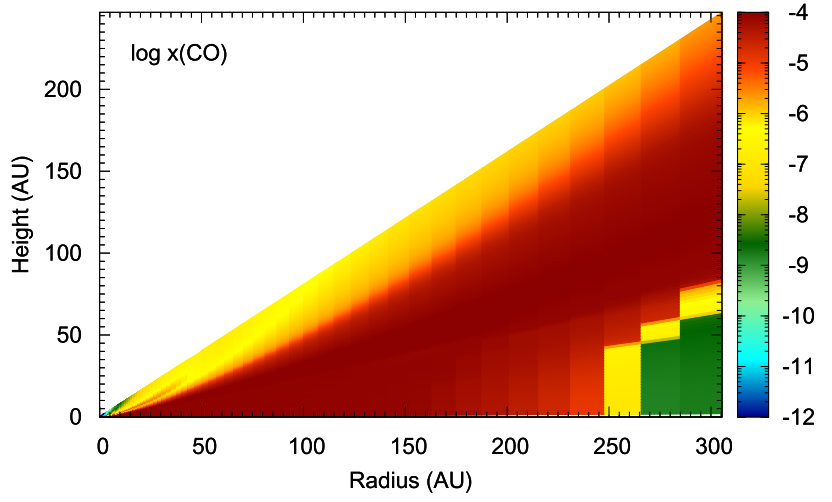
\includegraphics[width=0.33\linewidth]{walsh10_Xco.png}}\hfill%
  \subcaptionbox{\hco abundances}{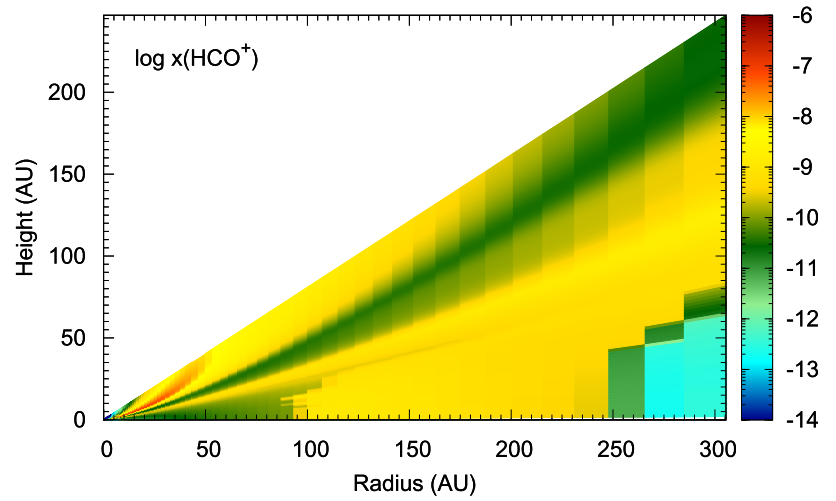
\includegraphics[width=0.33\linewidth]{walsh10_Xhco.png}}%
  \subcaptionbox{HCN abundances}{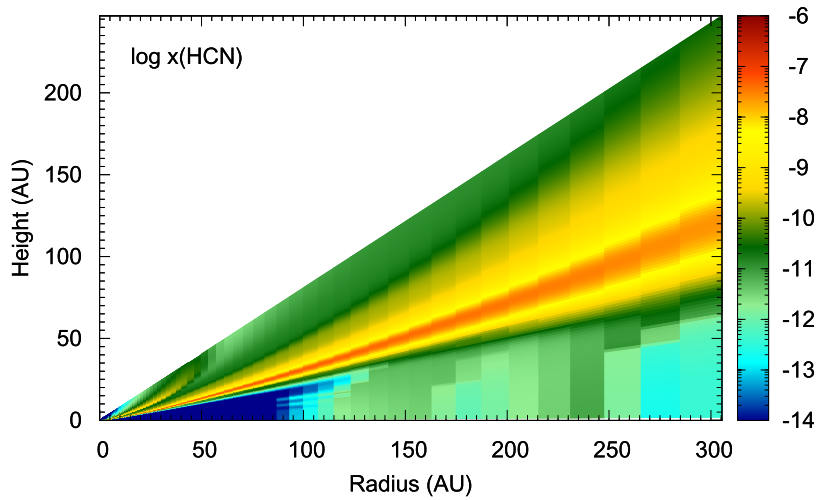
\includegraphics[width=0.33\linewidth]{walsh10_Xhcn.png}}%
  \hspace*{\fill}%
  \caption{Models from \citet{Walsh2013} showing radial and vertical distributions of CO, \hco, and HCN in a simulated disk around a T-Tauri star, being radiated by a nearby O star.}
  \label{fig:walsh-abundance-profs}
\end{figure}


\textit{Why does sam keep referencing Walsh2013 (which includes ionization) instead of Walsh2010, which is for an isolated disk?}



% Walsh et al. (2013) modeled the structure and emission from a disk surrounding a T Tauri star, being irradiated by a nearby O star and compared the gas line emission to that from an isolated disk. They found that, in general, line emission from the irradiated disk showed higher peak values due to the warmer disk. This was not the case for HCO+ which traces the cold, dense areas of the disk. Thus, the ratio of the HCN/HCO+ peak intensities can be used to roughly characterize the level of external irradiation, with HCN/HCO+ > 1 indicating an irradiated disk and HCN/HCO+ < 1 characteristic of an isolated disk.




\citet{Miotello2017} showed using isotopologues of CO that disks in Lupus have gas/dust ratios far below the literature value of 100, instead indicating that values of order 10 or even 1 are more appropriate. This was echoed by

Compare to slide 8/11 here:
https://www.cv.nrao.edu/rocks/pdf/S2-P4_rocks2013_millar.pdf


Good overview:
https://arxiv.org/pdf/1901.10862.pdf

Williams and Best: 100:1 is too high.
https://iopscience.iop.org/article/10.1088/0004-637X/788/1/59/pdf

Really good(-looking) paper on gas/dust ratio/chem models:
https://www.aanda.org/articles/aa/pdf/2017/03/aa29556-16.pdf




\section{Planet-Forming Potential}
\label{section:fitting_procedure}

In order to gauage a disk's planet forming potential, we may begin by referring to the MMSN

One way to contextualize the results presented in \S\ref{chap:analysis} is through the lens of planet formation. This analysis traditionally begins with a comparison to the MMSN, which is the density profile that our own Solar System would have if all our planets had gas added to them until their composition matched that of the Sun, then each planet's mass was spread out in a ring along its orbital path (as discussed in \S\ref{chap:introduction}). Integrating this mass leaves us with $M_\text{MMSN} \approx 0.01 M_\odot$. It is worth reiterating that this is an extremely rough metric, build on several assumptions, and that it does not reflect \textit{minimum} mass of a planet forming potential, but rather an approximation of the mass it would take for a disk like ours to form.

With the extremely large mass of $M = 0.36M_\odot$ that we measure in the CO line, it is needless to say that the disk's mass would not be its limiting factor in planet formation.





\section{Best Fit Temperature }
\label{section:fitting_procedure}

We begin by comparing to \citet{Factor2017}, in which they used similar methods of analysis to characterize another ONC proplyd, drawn from the same survey as our binary. Their results are presented in \ref{table:factor_fits}.


\begin{table}
  \centering
  \begin{threeparttable}
    \caption{Best-fit Results from \citet{Factor2017}}
    \label{table:factor_fits}
    \renewcommand{\arraystretch}{1.2}
    \begin{tabular}{l c c c c c }
      \toprule \toprule
      %\multirow{2}{*}{Parameter} & \multirow{2}{*}{Disk A}    & \multicolumn{2}{c}{Disk B} \\
      \multirow{2}{*}{Parameter} & \hco (thesis) & \hco (paper)  & HCN    & CO    & \hco \& CO \\
      \midrule %\midrule
      q                          & -0.02         & 0.17          & -0.18  & -0.33 & -0.24       \\
      T$_\text{atms}$ (\si{\K})  & 22            & 190           & 19     & 70    & 86          \\
      X$_\text{mol}$             & [-10]         & -10.07        & -6.7   & [-4]  & -10.04, [-4] \\
      \bottomrule
    \end{tabular}
    \begin{tablenotes}\footnotesize
      \item[*] CO values are from Sams paper. In his thesis, CO vals are [-0.3, 41, [-4]].
    \end{tablenotes}
  \end{threeparttable}
\end{table}

Comparing our results for disk A to theirs, we can see that our atmospheric temperature for the \hco fit is fairly well-aligned with their result. However, while our HCN fit is in quite close agreement with that of \hco, it is significantly higher than what they found.

Additionally, their temperature structures are systematically negative save for in the \hco line, where it is marginally positive. Ours, conversely, are systematically positive, and relatively larger than theirs. I don't know what to make of this\footnote{It also strikes me as strange that my temperatures are higher, since disk A's abundances for HCO+ are >two OoM higher than Sam's.}.


For the disk B fit, temperatures were notably higher across all lines, falling in the low 200's\footnote{Since the disk was not resolved, we were unable to fit for its temperature structure exponent, and thus fit it at -0.5 for all lines.}. Since


It is (maybe?) possible that this reflects the fact that our fits had different values for some of the fixed parameters. These include R$_{crit}$, which we fix at 100 and they fixed at 600 AU, as well as $z_q$ and $T_\text{mid}$, which they fit for and which together control how the temperature structure decays vertically (see \S\ref{subsection:physical_profs} for a more complete description). Since they fit multiple lines simultaneously, they were able to constrain these parameters, which is not possible in the case of single-line fitting. In a CO and \hco fit, they found values of $z_{q, 150} = 73$ AU and T$_{mid} = 24.7$ K, in comparison to our values of 29 and 19, respectively. \textit{Is this enough to make an appreciable difference? I don't know. It seems most likely to me that those drastically different R$_C$ values could explain the different q values, since if my disks are having their densities killed way earlier, then maybe they're struggling to match the flux levels further out. }

\textit{Another question about Sam's work: His paper and thesis have different values for the \hco and CO fits. He also makes no mention of the multi-line fits in his paper, which seems weird.}


% The expected value for q in a geometrically flat, optically thin disk is -0.5 while measured values vary from -0.6 to -0.3 (Dartois et al. 2003; Rosenfeld et al. 2012a,b)






\section{HCO$^+$, HCN Abundance Structures}
\label{section:fitting_procedure}










% The End

\chapter{Summary}
\label{chap:Summary}


We have presented ALMA observations tracing line emission CO(3-2), \hco(4-3), HCN(4-3), and CS(7-6) of d253-1536, a wide-separation binary system containing two young circumstellar protoplanetary disks in the M43 region of the Orion Nebula Cluster. We model the \hco, HCN, and CO emission using a gas model that assumes Keplerian rotation, local thermodynamic equilibrium, and hydrostatic equilibrium to develop synthetic images of a binary of model disks. We then use an affine-invariant Markov Chain Monte Carlo (MCMC) algorithm to explore parameter space and identify regions of best fit, comparing each model image to our data using a $\chi^2$ test. By fitting each line's emission, we are able to statistically characterize elements of the disks' chemical compositions and their temperature structures.

We find atmospheric temperatures that are atypically high relative to studies of other protoplanetary disks, as well as a temperature structure that increases radially, which is inconsistent with past studies of disks in low-mass star forming regions. Additionally, we find that in disk A, the binary's eastern disk, \hco and HCN abundances are nearly two orders of magnitude higher than in disk B, although the ratio of the molecules' abundances are almost exactly equal (near unity) in both disks. Finally, we note that the ratios of each molecule's integrated line flux in both disks is significantly lower than those predicted to be found in either an isolated disk or an irradiated disk \citep{Walsh2013}, perhaps reflecting a radially-dependent mass distribution for the different chemical species.

We also compared these results to results from \citet{Factor2017}, the only other forward-modeled study of line emission from an ONC proplyd. Our disks did not share the high abundance of HCN that they found, but their \hco line did match our large and radially-increasing temperatures. These deviations from literature (based on studies of disks in low-mass SFRs) hint at the potential for systematic variations between disks in low and high mass regions, and highlight the need for further study of disks in the Orion Nebula Cluster.
% REWORK: But, does “most of the literature” also equal “disks in low-mass SFRs”?  Remember, that’s what we’re trying to figure out.  If there is evidence for systematic differences between our disks (yours and Sam’s) and other disks in different environments, that’s really interesting!  The big caveat is: were the modeling methods similar enough that we are comparing apples to apples?  

% REWORK: Yeah, this last sentence sounds a little pie-in-the-sky.  I’d stick to the concrete question of: do we or do we not find evidence for chemical differences between disks in high-mass vs. low-mass SF regions.  I think the pie-in-the-sky piece that’s missing is mostly a discussion of how differences in chemical abundances might influence the properties of planets.  That’s a whole field of research that you haven’t even touched!  There are some good references in some of Karin Oberg’s group’s papers, and off the top of my head I know this is something that Nikku Madhusudhan has studied a lot, and I think he had a good review article about it a few years ago.  Those might be good places to start digging.  


\bigskip
\bigskip
\bigskip

I would like to thank my collaborators Meredith Hughes, Kevin Flaherty, Jessica Klusmeyer, and Cail Daley for their valuable contributions to this work. J.P. is funded by the Connecticut Space Grant's Undergraduate Research Fellowship, Undergraduate Scholarship, and Travel Grant, as well as Wesleyan University’s Research in the Sciences Fellowship.

This paper makes use of the following ALMA data: ADS/JAO.ALMA\#2011.0.00028.S. ALMA is a partnership of ESO (representing its member states), NSF (USA) and NINS (Japan), together with NRC (Canada), MOST and ASIAA (Taiwan), and KASI (Republic of Korea), in cooperation with the Republic of Chile. The Joint ALMA Observatory is operated by ESO, AUI/NRAO and NAOJ. The National Radio Astronomy Observatory is a facility of the National Science Foundation operated under cooperative agreement by Associated Universities, Inc.


This project made heavy use of the following open-source analysis tools: Pandas \citep{McKinney2010,McKinney2011}, NumPy \citep{VanDerWalt2011}, emcee \citep{ForemanMackey2013}

\appendix
%-----------------------------------------------------------------------------------------------------------------------------------------
%%BIBLIOGRAPHY:
\fancypagestyle{plain}{%
% clear all header and footer fields, we don't want these for the bibliography
\fancyhf{}
% except we want the page number to show up in the center of the footer:
\fancyfoot[C]{\thepage}

\renewcommand{\headrulewidth}{0pt}
\renewcommand{\footrulewidth}{0pt}}
\pagestyle{plain}

%change title spacing once again, for the bibliography:
\titlespacing*{\chapter}{0pt}{-.75in}{*3}

%Add the bibliography
\addcontentsline{toc}{chapter}{\textbf {Bibliography}}

%The default for BibTex (the bibliography builder in LaTeX) is to not include citations that are in your bibliography file, but that you don't cite anywhere in the paper.  This changes that setting, so that all papers show up in the bibliography, whether or not you referenced them:
\nocite{*}

%Insert the bibliography (in this case, my file name was also "bibliography" if not, your line would read:\bibliography{my_workscited_filename} or whatever:
\bibliographystyle{apj}
\bibliography{Thesis-References}
\printbibliography


\end{document}
